\documentclass[a4paper, 12pt]{article}
\usepackage[utf8]{inputenc}
\renewcommand\familydefault{\sfdefault}
\usepackage[T1]{fontenc}
\usepackage[francais]{babel}
\usepackage[left=2.5cm,top=2.5cm,right=2.5cm,bottom=2.5cm]{geometry}
\usepackage[onehalfspacing]{setspace}
\usepackage{graphicx}
\usepackage[usenames, dvipsnames]{xcolor}
\definecolor{mygray}{gray}{0.95}

\usepackage{minted}
\usemintedstyle{colorful}
\usepackage{float}
\floatplacement{figure}{H}
\usepackage{authblk}
\usepackage{enumitem}
\setlist[enumerate]{label*=\arabic*.}
\usepackage{hyperref}
\hypersetup{
    colorlinks,
    citecolor=black,
    filecolor=black,
    linkcolor=black,
    urlcolor=blue
}

\usepackage{caption}
\newenvironment{code}{\captionsetup{type=listing}}{}
\usepackage{array}
\usepackage{etoolbox}
\patchcmd{\thebibliography}{\section*{\refname}}{}{}{}

\usepackage{dirtree}
\usepackage{tabularx}

\usepackage{glossaries}
	\let\oldnewacronym\newacronym
	\newcommand*{\provideacronym}[3]{%
	  \ifglsentryexists{#1}{%
	  }{%
	    \oldnewacronym{#1}{#2}{#3}%
	  }%
	}
\makeglossaries

\usepackage{fancyhdr}
\pagestyle{fancy}
\fancyhf{}
\lhead{\leftmark}
\lfoot{Steven Liatti}
\rfoot{\thepage}
\renewcommand{\footrulewidth}{1pt}

\usepackage{pdfpages}

\begin{document}

\title{TagFS \protect\\ Système d'étiquetage des fichiers avec Rust}
\author{Steven Liatti}
\affil{\small Projet de bachelor - Prof. Florent Glück}
\affil{\small Hepia ITI 3\up{ème} année}
\maketitle

% \subparagraph{Résumé}
% Le but de ce projet est de concevoir et développer un "moteur de gestion de tags" pouvant gérer des dizaines de milliers
% de fichiers et tags associés de manière efficace, en Rust. Le stockage des tags utilisera le mécanisme des "extended
% attributes" disponibles dans la plupart des systèmes de fichiers modernes. Le moteur d'indexation devra surveiller les
% fichiers modifiés, créés, ou supprimés afin d'indexer les tags avec un minimum de latence (temps réel). Si le temps le
% permet, le système développé sera intégré à un environnement desktop choisi (Gnome, KDE, etc.).

% \begin{figure}
% 	\begin{center}
% 		
\includegraphics[width=0.43\textwidth]{images/title.png}
% 	\end{center}
% \end{figure}

\begin{figure}[!b]
	\centering
	\begin{minipage}{.5\textwidth}
		\centering
		
\includegraphics[width=.7\linewidth]{images/hepia.jpg}
	\end{minipage}%
	\begin{minipage}{.5\textwidth}
		\centering
		
\includegraphics[width=.7\linewidth]{images/hesso.jpg}
	\end{minipage}
\end{figure}
\newpage
\thispagestyle{empty}
\mbox{}

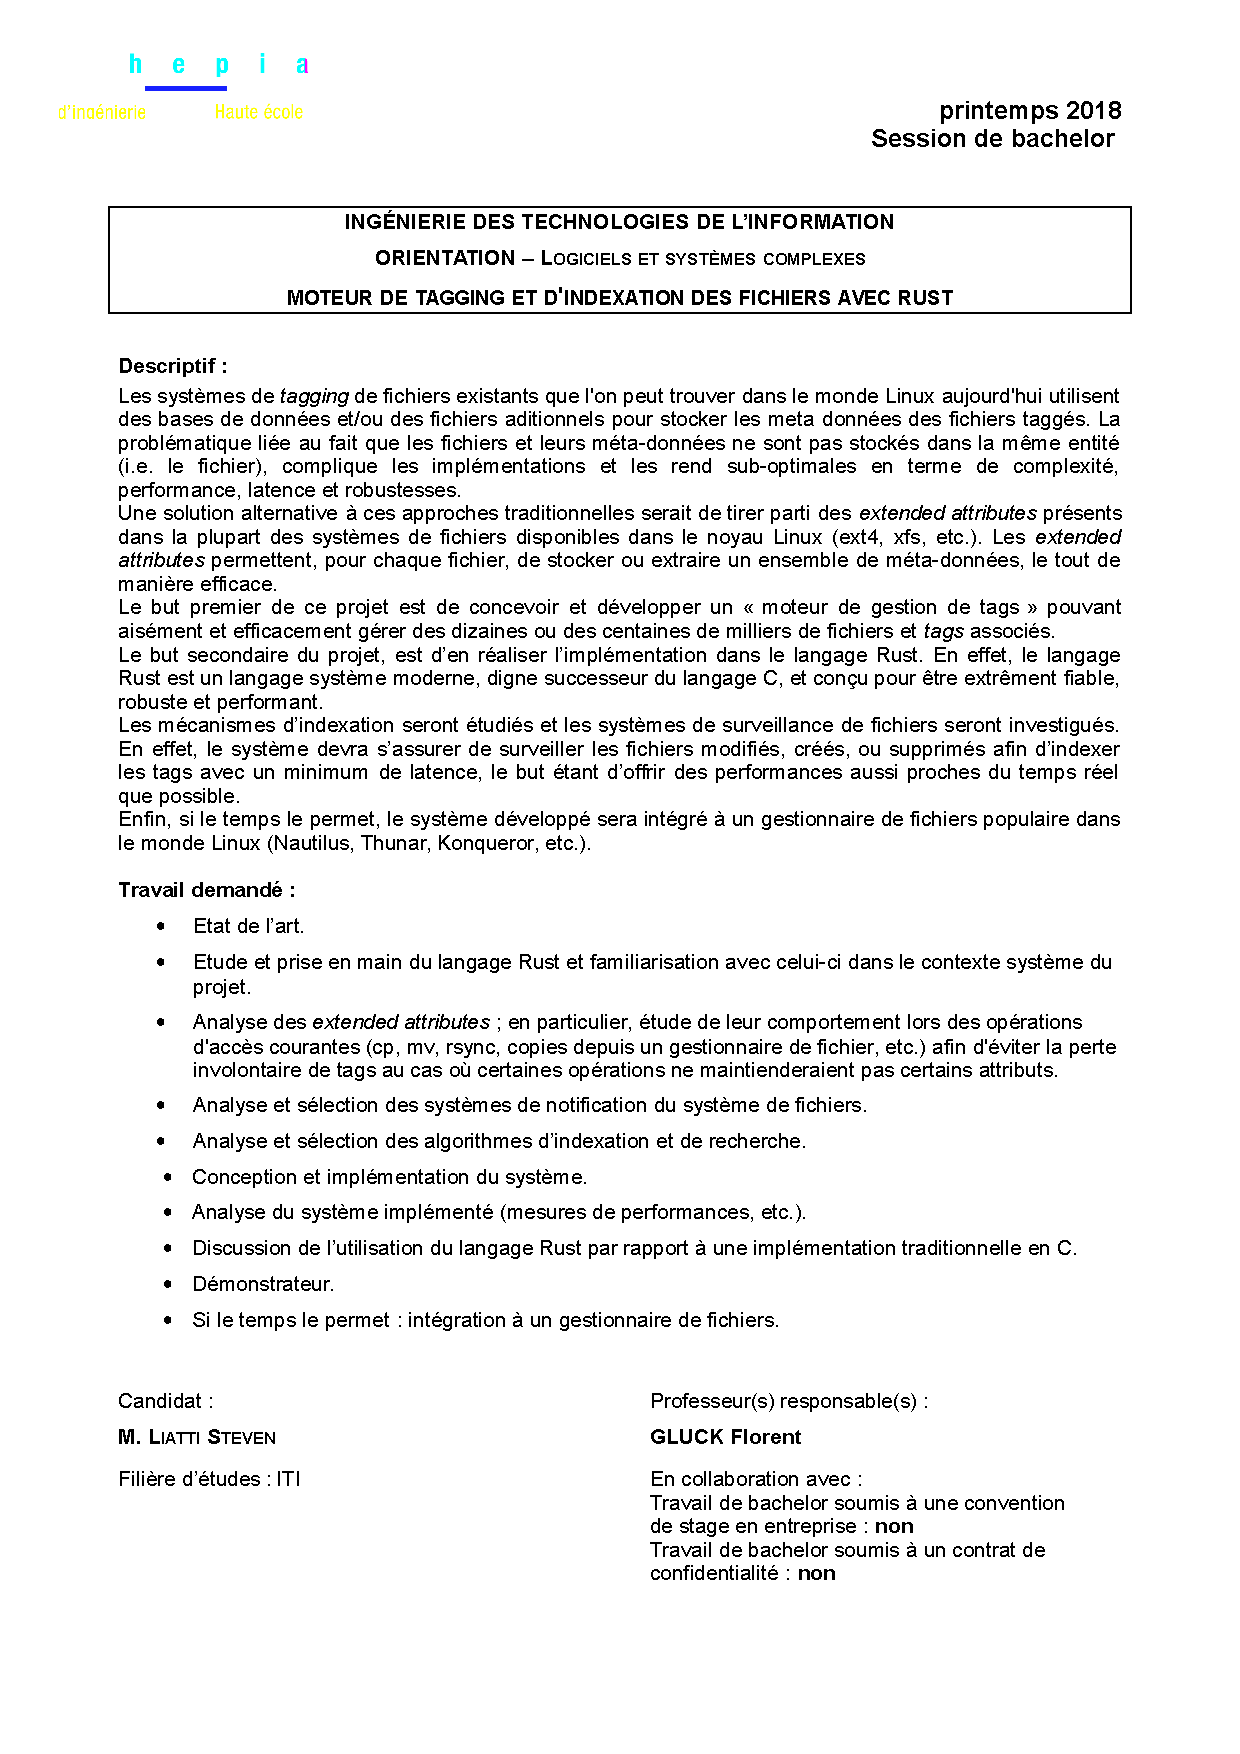
\includepdf[pages=1]{enonce.pdf}
\addcontentsline{toc}{subsection}{Énoncé du travail}
\newpage

\subsection*{Résumé} %-----------------------------------------------------------------------------------------------
\addcontentsline{toc}{subsection}{Résumé}
% TODO: résumé

\newpage

% \setcounter{tocdepth}{2}
\addcontentsline{toc}{subsection}{Table des matières}
\tableofcontents
\subsubsection*{Annexes . . . . . . . . . . . . . . . . . . . . . . . . . . . . . . . . . . . . . . . . . . . Volume 2}
\newpage
\addcontentsline{toc}{subsection}{Table des figures}
\listoffigures
\newpage
\renewcommand{\listtablename}{Table des tables}
\addcontentsline{toc}{subsection}{Table des tables}
\listoftables
\newpage
\renewcommand\listoflistingscaption{Table des listings de code source}
\addcontentsline{toc}{subsection}{Table des listings de code source}
\listoflistings
\newpage

\subsection*{Conventions typographiques} %-----------------------------------------------------------------------------------------------
\addcontentsline{toc}{subsection}{Conventions typographiques}
Lors de la rédaction de ce document, les conventions typographique ci-dessous ont
été adoptées.
\begin{itemize}[label=\textbullet]
	\item Tous les mots empruntés à la langue anglaise ou latine ont été écrits en \textit{italique}
	\item Toute référence à un nom de fichier (ou dossier), un chemin d'accès, une 
    utilisation de paramètre, variable, commande utilisable par l'utilisateur, ou extrait de code 
    source est écrite avec une police d'écriture à \mintinline{text}{chasse fixe}.
	\item Tout extrait de fichier ou de code est écrit selon le format suivant:
    \bigbreak
    \begin{code}
        \begin{minted}[bgcolor=mygray,breaklines,breaksymbol=,linenos,frame=single,stepnumber=1,tabsize=2]{rust}
fn main() {
    println!("Hello, world!");
}
        \end{minted}
    \end{code}
    \item Dans les listings, les lignes précédées d'un "\$" sont exécutées dans un shell.
\end{itemize}

\subsection*{Structure du document} %-----------------------------------------------------------------------------------------------
\addcontentsline{toc}{subsection}{Structure du document}
Le présent document commence par l'introduction, rappelant les motivations du projet et les buts à 
atteindre. Il aborde ensuite les applications existantes fournissant un service similaire au but du 
projet, mais avec quelques limitations pour la plupart. Il poursuit par une section sur l'architecture 
logicielle du système final, avec ses différents composants et besoins. Après, une analyse technologique du 
langage Rust et des outils utilisés pour la réalisation technique sera faite. La section suivante illustre 
la réalisation technique en elle-même, avec les deux programmes réalisés. Le système est testé dans 
la section d'après, expliquant le protocole et le résultat des tests. Finalement, le document se 
termine par une section de discussion des résultats, de l'état du projet, des améliorations futures 
et des différences entre Rust et C et une dernière section de conclusion. La dernière section 
est réservée aux références.

\subsection*{Remerciements} %-----------------------------------------------------------------------------------------------
\addcontentsline{toc}{subsection}{Remerciements}
Mes remerciements vont en premier lieu à ma compagne, Marie Bessat, pour son infinie patience et ses encouragements.
Je remercie aussi ma famille et mes proches pour leur soutien tout au long de mes études et 
lors de la réalisation de ce travail. Je tiens à remercier tous mes professeurs pour leurs 
enseignements et tout particulièrement M. Florent Glück pour le suivi du projet et ses précieux 
conseils ainsi que M. Orestis Malaspinas pour les conseils sur le langage Rust. J'aimerais remercier aussi 
M. Joël Cavat, assistant ITI à l'hepia, pour m'avoir conseillé et m'avoir prêté son très bon 
cours sur les Graphes et Réseaux de M. Jean-Francois Hêche, que je remercie indirectement. 
Je tiens finalement à remercier mes collègues de classe pour leur camaraderie et aide durant mes 
études et mon travail de bachelor.

\newpage

% TODO: parcourir le texte pour voir si remplacement par acronyme + premier acronyme de section en toutes lettres
\newacronym{xattr}{XATTR}{\textit{Extended Attributes}, Attributs étendus : voir section 
    \ref{extended_attributes}}
\newacronym{api}{API}{\textit{Application Programming Interface}, Interface de programmation : 
    services offerts par un programme producteur à d'autres programmes consommateurs}
\newacronym{syscall}{SYSCALL}{\textit{System call}, Appel système : lorsqu'un programme a besoin d'un 
    accès privilégié à certaines parties du système d'exploitation (système de fichier, mémoire, 
    périphériques), il demande au noyau d'exécuter l'opération voulue pour lui}
\newacronym{fs}{FS}{\textit{File System}, Système de fichiers : organisation logique des fichiers 
    physiques sur le disque}
\newacronym{os}{OS}{\textit{Operating System}, Système d'exploitation : couche logicielle entre le 
    matériel d'un ordinateur et les applications utilisateurs. Offre des abstractions pour la gestion 
    des processus, des fichiers et des périphériques entre autres}
\newacronym{cli}{CLI}{\textit{Command Line Interface}, Interface en ligne de commande : interface 
    homme-machine en mode texte : l'utilisateur entre des commandes dans un terminal et l'ordinateur 
    répond en exécutant les ordres de l'utilisateur et en affichant le résultat de l'opération}
\newacronym{gui}{GUI}{\textit{Graphical User Interface}, Interface graphique : moyen d'intéragir avec 
    un logiciel où les contrôles et objets sont manipulables. S'oppose à l'interface en ligne de commande 
    (\acrshort{cli})}
\printglossary[type=\acronymtype,title={Acronymes}]
\newpage


\section{Introduction} %-----------------------------------------------------------------------------------------------
%%%%%%%%%%%%%%%%%%%%%%%%%%%%%%%%%%%%%%%%%%%%%%%%%%%%%%%%%%%%%%%%%%%%%%%%%%%%%%%%%%%%%%%%%%%%%%%%%%%
%%%%%%%%%%%%%%%%%%%%%%%%%%%%%%%%%%%%%%%%%%%%%%%%%%%%%%%%%%%%%%%%%%%%%%%%%%%%%%%%%%%%%%%%%%%%%%%%%%%
\subsection{Motivations}
Avec l'augmentation de la puissance de calcul et la capacité de stockage de masse grandissante à un 
prix raisonnable, nos ordinateurs gèrent des quantités de fichiers très importantes, de l'ordre du 
millier ou du million de fichiers. Que ce soit des images, des documents ou de la musique, les 
réserves de stockage de fichiers semblent sans fin. Dès lors se pose la question de l'organisation 
de ces nombreux fichiers. Comment doit-on ordonner ses photos personnelles ? Par date, par lieu, 
par thème ? Ce sont trois bonnes réponses, mais malheureusement pour l'utilisateur, les \acrshort{os} 
d'aujourd'hui ne proposent qu'une seule manière native d'organiser ses fichiers : 
la classique hiérarchie de répertoires, sous-répertoires et fichiers, sous la forme d'une arboresence.
\bigbreak
Comment retrouver rapidement la photo de votre chat dormant sur votre balcon au début de sa vie 
dans une masse de plus de 10'000 images ? Comment classer son répertoire d'études, un répertoire 
pour les cours, un autre pour les travaux pratiques, ou pour chaque cours, deux sous-répertoires 
"théorie" et "pratique" ? Comment récupérer une chanson sans connaître son titre ni l'artiste mais 
en connaissant le genre ? Une solution à ces problèmes est de donner la possibilité à l'utilisateur 
d'apposer une ou plusieurs étiquettes, ou "tags", sur ses fichiers et de lui fournir une interface 
avec laquelle il pourra aisément retrouver ses fichiers. Il doit garder le contrôle sur ses fichiers 
et pouvoir les manipuler comme il l'a toujours fait. Les tags doivent être stockés avec les fichiers, 
pour qu'ils ne soient pas perdus en cas de grand changement dans le système. L'utilisation des 
attributs étendus, ou \textit{extended attributes} est la manière la plus naturelle de répondre à 
ce dernier besoin : les tags "voyagent" ainsi avec les fichiers. Nous verrons qu'il existe 
des applications résolvant en partie ce problème. Finalement, cette interface doit être performante et fiable. 
\bigbreak
Ces deux qualificatifs, performant et fiable, résument le langage de programmation Rust. Rust est 
un langage de programmation moderne fort d'une communauté grandissante et passionnée. Il est très 
performant, proche ou meilleur que C selon les situations. Il est fiable grâce à ses règles strictes 
sur l'utilisation de la mémoire et son compilateur très intelligent. C'est un langage totalement 
adapté à notre situation. À travers ce travail, le lecteur pourra se faire une illustration des 
possibilités offertes par Rust.
\bigbreak
Le but de ce travail est donc de concevoir et développer un moteur de gestion des tags répondant 
aux besoins cités précédemment et d'apprendre les notions de Rust nécessaires à sa réalisation.
%%%%%%%%%%%%%%%%%%%%%%%%%%%%%%%%%%%%%%%%%%%%%%%%%%%%%%%%%%%%%%%%%%%%%%%%%%%%%%%%%%%%%%%%%%%%%%%%%%%
%%%%%%%%%%%%%%%%%%%%%%%%%%%%%%%%%%%%%%%%%%%%%%%%%%%%%%%%%%%%%%%%%%%%%%%%%%%%%%%%%%%%%%%%%%%%%%%%%%%
\newpage
\subsection{Buts}
Avec plus de détails, les buts de ce projet sont les suivants :
\begin{itemize}
    \item Étudier et s'approprier le langage Rust pour la réalisation d'une application système sous Linux.
    \item Répertorier les applications existantes permettant d'étiqueter les fichiers.
    \item Étudier les \textit{extended attributes} lors des manipulation courantes sur les fichiers.
    \item Explorer les méthodes de surveillance du \acrshort{fs}.
    \item Analyser les moyens d'indexer une arboresence de fichiers.
    \item Concevoir et implémenter un système répondant aux motivations. Il devra être performant, 
        utilisable en temps réel et gérer de nombreux fichiers, répertoires et tags.
    \item Mesurer les performances de ce système.
    \item Réaliser une démonstration.
\end{itemize}

\newpage

\section{Analyse de l'existant} %-----------------------------------------------------------------------------------------------
Dans cette section, nous allons analyser les principales solutions existantes, qu'elles soient 
sous la forme d'applications utilisateur ou intégrées directement dans un \acrshort{os}.
Jean-Francois Dockes en dresse également une liste avec avantages et inconvénients sur son site 
\cite{ref3}. Ce que nous recherchons est une application \textit{open source}, fonctionnant sur Linux, 
stockant les tags dans les \acrshort{xattr}, ne modifiant pas les fichiers et performante.

%%%%%%%%%%%%%%%%%%%%%%%%%%%%%%%%%%%%%%%%%%%%%%%%%%%%%%%%%%%%%%%%%%%%%%%%%%%%%%%%%%%%%%%%%%%%%%%%%%%
%%%%%%%%%%%%%%%%%%%%%%%%%%%%%%%%%%%%%%%%%%%%%%%%%%%%%%%%%%%%%%%%%%%%%%%%%%%%%%%%%%%%%%%%%%%%%%%%%%%
\subsection{Applications utilisateur}
%%%%%%%%%%%%%%%%%%%%%%%%%%%%%%%%%%%%%%%%%%%%%%%%%%%%%%%%%%%%%%%%%%%%%%%%%%%%%%%%%%%%%%%%%%%%%%%%%%%
%%%%%%%%%%%%%%%%%%%%%%%%%%%%%%%%%%%%%%%%%%%%%%%%%%%%%%%%%%%%%%%%%%%%%%%%%%%%%%%%%%%%%%%%%%%%%%%%%%%
\subsubsection{TMSU}
TMSU \cite{ref15} est un outil en ligne de commande (\acrshort{cli}) qui permet d'attribuer des tags à des 
fichiers et d'exécuter des recherches par tags. On commence par initialiser TMSU dans le dossier choisi. 
Une commande liste les tags associés à un ou 
plusieurs fichiers et une autre liste les fichiers qui possèdent le ou les tags donnés. TMSU offre 
la possibilité à l'utilisateur de "monter" un \acrshort{fs} virtuel avec FUSE (Filesystem in 
UserSpacE). L'outil est rapide et efficace, mais il comporte quelques défauts :
\begin{itemize}
    \item Pas d'interface graphique.
    \item Dépendance à FUSE pour monter le \acrshort{fs} virtuel.
    \item Stockage des tags dans une base de données SQLite : si la base est perdue, les tags également.
\end{itemize}

%%%%%%%%%%%%%%%%%%%%%%%%%%%%%%%%%%%%%%%%%%%%%%%%%%%%%%%%%%%%%%%%%%%%%%%%%%%%%%%%%%%%%%%%%%%%%%%%%%%
%%%%%%%%%%%%%%%%%%%%%%%%%%%%%%%%%%%%%%%%%%%%%%%%%%%%%%%%%%%%%%%%%%%%%%%%%%%%%%%%%%%%%%%%%%%%%%%%%%%
\subsubsection{Tagsistant}
Tagsistant \cite{ref16} est autre outil \acrshort{cli} de gestion de tags. Il dépend de FUSE et d'une base 
de données (SQLite ou MySQL) pour fonctionner. Comme pour TMSU, il faut donner un répertoire à Tagsistant 
pour son usage interne. À l'intérieur de ce dernier, se trouvent différents répertoires :
\dirtree{%
.1 /.
.2 alias --- Répertoire contenant les requêtes les plus courantes.
.2 archive --- Répertoire listant les fichiers.
.2 relations --- Répertoire contenant les relations entre les tags et fichiers.
.2 stats --- Répertoire contenant des infos sur l'utilisation de Tagsistant.
.2 store --- Répertoire où sont gérés les fichiers et ajoutés les tags.
.2 tags --- Répertoire de gestion des tags.
}
\bigbreak
Chaque répertoire a un rôle bien précis. Tout se fait avec le terminal et des commandes usuelles 
(\mintinline{text}{cp}, \mintinline{text}{ls}, \mintinline{text}{mkdir}, etc.). Dans Tagsistant, 
un répertoire créé dans le répertoire \mintinline{text}{tags} correspond à un tag. On se retrouve 
finalement avec une arborescence de tags et de fichiers \cite{ref17}. Bien que cet outil soit 
performant d'un point de vue de la rapidité d'exécution, il comporte les défauts de TMSU ainsi que 
des nouveaux :
\begin{itemize}
    \item Pas d'interface graphique.
    \item Dépendance à FUSE pour monter le \acrshort{fs} virtuel.
    \item Stockage des tags dans une base de données : si la base est perdue, les tags également.
    \item Utilisation des différents répertoires peu intuitive.
    \item Tous les fichiers sont contenus dans un seul répertoire et leur nom est modifié pour les 
        besoins internes de l'application. Obligation de passer par l'application pour accéder aux 
        fichiers.
\end{itemize} 

%%%%%%%%%%%%%%%%%%%%%%%%%%%%%%%%%%%%%%%%%%%%%%%%%%%%%%%%%%%%%%%%%%%%%%%%%%%%%%%%%%%%%%%%%%%%%%%%%%%
%%%%%%%%%%%%%%%%%%%%%%%%%%%%%%%%%%%%%%%%%%%%%%%%%%%%%%%%%%%%%%%%%%%%%%%%%%%%%%%%%%%%%%%%%%%%%%%%%%%
\subsubsection{TaggedFrog}
TaggedFrog \cite{ref18} est un programme disponible sur Windows uniquement et ne partage pas ses sources.
Son fonctionnement interne n'est pas documenté. L'interface est agréable, on peut ajouter des fichiers 
par \textit{Drag \& Drop}. L'interface créé au fur et à mesure un "nuage" de tags, comme on peut le retrouver sur 
certains sites web. On peut exécuter des recherches sur les tags et les fichiers. On peut supposer que 
TaggedFrog maintient une base de données des tags associés aux fichiers, ce qui ne correspond à nouveau 
pas à nos besoins.
\begin{figure}
    \begin{center}
        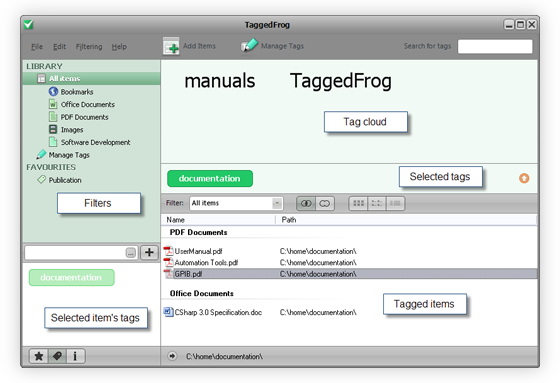
\includegraphics[width=0.8\textwidth]{images/taggedfrog.png}
    \end{center}
    \caption{TaggedFrog en utilisation \cite{ref18}}
    \label{taggedfrog}
\end{figure}

%%%%%%%%%%%%%%%%%%%%%%%%%%%%%%%%%%%%%%%%%%%%%%%%%%%%%%%%%%%%%%%%%%%%%%%%%%%%%%%%%%%%%%%%%%%%%%%%%%%
%%%%%%%%%%%%%%%%%%%%%%%%%%%%%%%%%%%%%%%%%%%%%%%%%%%%%%%%%%%%%%%%%%%%%%%%%%%%%%%%%%%%%%%%%%%%%%%%%%%
\subsubsection{TagSpaces}
TagSpaces \cite{ref13} est un programme avec une \acrshort{gui} permettant d'étiqueter ses fichiers avec des tags. 
L'application est agréable à utiliser, on commence par connecter un emplacement qui fera office de dossier de 
destination aux fichiers. On peut ajouter ou créer des fichiers depuis l'application. Les fichiers 
existants ajoutés depuis l'application sont copiés dans le dossier (cela créé donc un doublon). 
Sur le panneau de gauche se situe la zone de gestion des tags. TagSpaces ajoute automatiquement 
certains tags dits "intelligents" aux fichiers nouvellement créés avec l'application (par exemple 
un tag avec la date de création).
\begin{figure}
    \begin{center}
        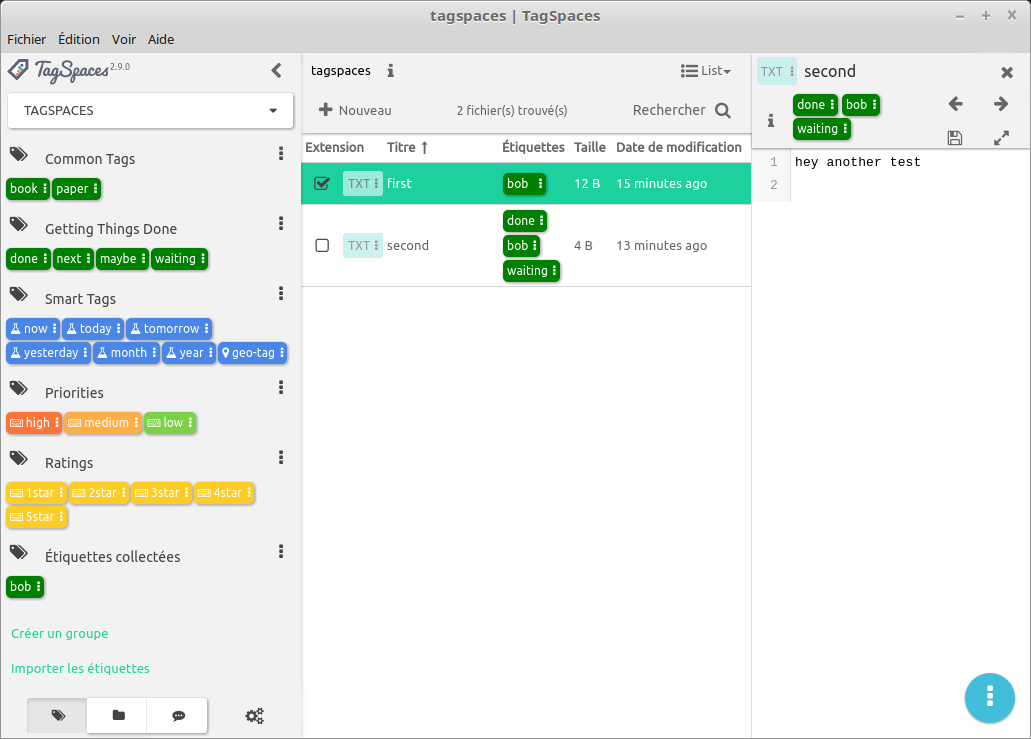
\includegraphics[width=0.8\textwidth]{images/tagspaces.png}
    \end{center}
    \caption{TagSpaces en utilisation}
    \label{tagspaces}
\end{figure}
Globalement, l'application est fonctionnelle et \textit{user friendly}. Cependant, deux points noirs 
sont à déplorer :
\begin{enumerate}
    \item L'application copie les fichiers déjà existants sélectionnés par l'utilisateur, ce qui 
        créé une contrainte supplémentaire dans la gestion de ses fichiers personnels.
    \item TagSpaces stocke les tags directement dans le nom du fichier, modifiant ainsi son nom \cite{ref14}.
        Bien que pratique dans le cas d'une synchronisation à l'aide d'un service cloud, 
        le fichier devient dépendant de TagSpaces. Si l'utilisateur décide de changer son nom sans 
        respecter la nomenclature interne, il risque de perdre les tags associés au fichier.
\end{enumerate}

%%%%%%%%%%%%%%%%%%%%%%%%%%%%%%%%%%%%%%%%%%%%%%%%%%%%%%%%%%%%%%%%%%%%%%%%%%%%%%%%%%%%%%%%%%%%%%%%%%%
%%%%%%%%%%%%%%%%%%%%%%%%%%%%%%%%%%%%%%%%%%%%%%%%%%%%%%%%%%%%%%%%%%%%%%%%%%%%%%%%%%%%%%%%%%%%%%%%%%%
\subsection{Fonctionnalités disponibles dans l'\acrshort{os}}

%%%%%%%%%%%%%%%%%%%%%%%%%%%%%%%%%%%%%%%%%%%%%%%%%%%%%%%%%%%%%%%%%%%%%%%%%%%%%%%%%%%%%%%%%%%%%%%%%%%
%%%%%%%%%%%%%%%%%%%%%%%%%%%%%%%%%%%%%%%%%%%%%%%%%%%%%%%%%%%%%%%%%%%%%%%%%%%%%%%%%%%%%%%%%%%%%%%%%%%
\subsubsection{Windows}
À partir de Windows Vista, Microsoft a donné la possibilité aux utilisateurs d'ajouter des 
méta-données aux fichiers; parmi ces méta-données se trouvent les tags. Il existe une fonctionnalité 
appelée \textit{Search Folder} qui permet de créer un dossier virtuel contenant le résultat d'une 
recherche sur les noms de fichiers ou d'autres critères \cite{ref19}. Depuis Windows 8, l'utilisateur 
a la possibilité d'ajouter des méta-données à certains types de fichiers (ceux de la suite office 
par exemple), dont des tags. Il peut par la suite exécuter des recherches ciblées via recherche de 
l'explorateur de fichiers Windows du type \mintinline{text}{meta:value} \cite{ref20}. C'est 
dommage que Windows ne prenne pas en compte davantage de types de fichiers, comme les PDFs ou les 
fichiers \mintinline{text}{.txt}.

%%%%%%%%%%%%%%%%%%%%%%%%%%%%%%%%%%%%%%%%%%%%%%%%%%%%%%%%%%%%%%%%%%%%%%%%%%%%%%%%%%%%%%%%%%%%%%%%%%%
%%%%%%%%%%%%%%%%%%%%%%%%%%%%%%%%%%%%%%%%%%%%%%%%%%%%%%%%%%%%%%%%%%%%%%%%%%%%%%%%%%%%%%%%%%%%%%%%%%%
\subsubsection{macOS}\label{existant_macOS}
macOS possède son propre système pour étiqueter des fichiers. Il est intégré depuis la version 
OS X 10.9 Mavericks. Depuis l'explorateur de fichiers, l'utilisateur a la possibilité 
d'ajouter, modifier, supprimer et rechercher des tags. Les fichiers peuvent avoir plusieurs tags 
associés. Un code couleur permet de plus facilement se souvenir et visualiser les tags attribués. 
Dans l'explorateur de fichiers, les tags se retrouvent sur le bas côté, pour y accéder plus 
rapidement. 
\begin{figure}
    \begin{center}
        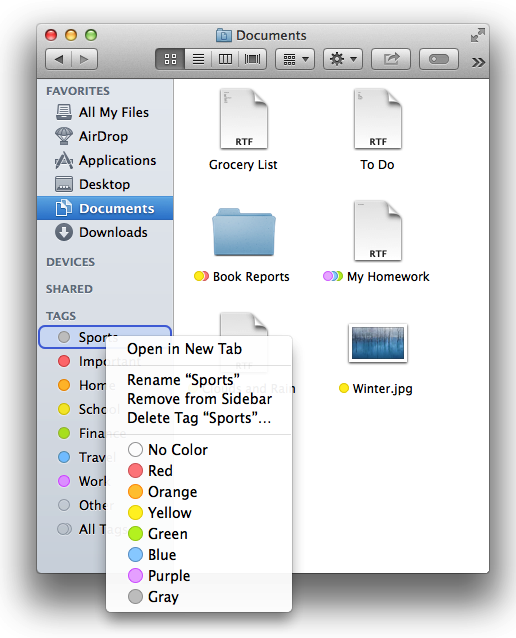
\includegraphics[width=0.8\textwidth]{images/macos_tags.png}
    \end{center}
    \caption{Vue et gestion d'un tag dans le Finder macOS \cite{ref5}}
    \label{macos_tags}
\end{figure}
Lorsque l'on clique sur un tag, une recherche Spotlight est effectuée. Spotlight est le moteur de 
recherche interne à macOS. Spotlight garde un index des tags, fournissant un accès rapide aux 
fichiers correspondants \cite{ref9}.
Tous ces tags peuvent se synchroniser sur les différents "iDevices" via iCloud. Finalement, 
un menu de réglages permet la gestion des tags (affichage, suppression, etc.) \cite{ref5}, 
\cite{ref6}. L'implémentation de ce système utilise les extended attributes (voir section 
\ref{extended_attributes}) pour stocker les tags. Les différents tags se trouvent dans l'attribut 
\mintinline{shell}{kMDItemUserTags}, listés les uns à la suite des autres. Via le Terminal, à 
l'aide de la commande \mintinline{shell}{mdls}, nous pouvons afficher la liste des tags associés à 
un fichier, nommé "Hello" pour l'exemple :
\bigbreak
\begin{code}
    \begin{minted}[bgcolor=mygray,breaklines,breaksymbol=,linenos,frame=single,stepnumber=1,tabsize=2]{shell}
% mdls -name kMDItemUserTags Hello 
kMDItemUserTags = (
    Green,
    Red,
    Essential
)
    \end{minted}
    \caption{\mintinline{shell}{mdls} listant les tags d'un fichier sous macOS \cite{ref7}}
\end{code}
\bigbreak
Ici, ce fichier "Hello" est étiqueté avec trois tags, "Green", "Red" et "Essential". Le fait que 
l'indexation est réalisée avec Spotlight implique une réindexation des fichiers dans le cas d'un 
changement de nom pour un tag donné sous macOS. Le framework système \mintinline{text}{FSEvents} 
donne une solution partielle : c'est une \acrshort{api} (utilisée également par Spotlight) qui offre aux 
applications la possibilité d'être notifiées si un changement a eu lieu sur un dossier (un événement 
toutes les 30 secondes). \mintinline{text}{FSEvents} maintient des logs de ces changements dans 
des fichiers, les applications peuvent ainsi retrouver l'historique des changements quand elles 
le souhaitent \cite{ref10}.

\newpage

\section{Architecture} %-----------------------------------------------------------------------------------------------
Le système global est composé de quatre entités distinctes, décrites dans les sous-sections suivantes.

%%%%%%%%%%%%%%%%%%%%%%%%%%%%%%%%%%%%%%%%%%%%%%%%%%%%%%%%%%%%%%%%%%%%%%%%%%%%%%%%%%%%%%%%%%%%%%%%%%%
%%%%%%%%%%%%%%%%%%%%%%%%%%%%%%%%%%%%%%%%%%%%%%%%%%%%%%%%%%%%%%%%%%%%%%%%%%%%%%%%%%%%%%%%%%%%%%%%%%%
\subsection{Gestion des tags}
La gestion physiques des tags stockés dans les attributs étendus (\acrshort{xattr}) est une fonctionnalité indépendante du 
reste du système. Comme vu dans la section \ref{extended_attributes}, des outils système existent pour 
manipuler les \acrshort{xattr} des fichiers. Cependant, pour offrir un plus haut niveau d'abstraction, 
une cohérence sur le nommage des tags pour l'indexation et plus de confort pour l'utilisateur final, 
un outil devient nécessaire pour la gestion des tags. Cet outil se présente, sous sa forme de base, 
comme un programme en ligne de commande. Il doit, au minimum, offrir la possibilité de lire les tags 
contenus dans les fichiers et ajouter et supprimer les tags donnés en entrée par l'utilisateur. 
Il devra pouvoir manipuler plusieurs tags et fichiers simultanément. D'un point de vue algorithmique 
et structures de données, cette partie n'est pas particulièrement ardue.

%%%%%%%%%%%%%%%%%%%%%%%%%%%%%%%%%%%%%%%%%%%%%%%%%%%%%%%%%%%%%%%%%%%%%%%%%%%%%%%%%%%%%%%%%%%%%%%%%%%
%%%%%%%%%%%%%%%%%%%%%%%%%%%%%%%%%%%%%%%%%%%%%%%%%%%%%%%%%%%%%%%%%%%%%%%%%%%%%%%%%%%%%%%%%%%%%%%%%%%
\subsection{Indexation des fichiers et des tags}
L'indexation des fichiers et des tags associés est l'un des deux piliers du système. Il faut créer 
un index des relations entre les tags et les fichiers. Le terme "index" utilisé ici ne 
prend pas son sens littéraire exact, \textit{id est} la liste des termes importants 
d'un livre avec la liste des pages dans lesquels ils apparaissent. Dans notre situation, il se 
rapproche plus de son utilisation pour les bases de données : c'est une structure de données 
permettant de retrouver rapidement les données, dans notre cas, récupérer rapidement la relation 
entre tags et fichiers. Deux architectures ont été imaginées pour l'indexation des tags et des fichiers, 
elles sont décrites dans les deux sous-sections suivantes. La table \ref{table_evenements_possibles} liste 
les événements qui se produisent lors d'une utilisation normale du \acrshort{fs} en leur attribuant 
un numéro. Ces numéros sont repris et utilisés pour alléger la lecture des tables \ref{table_architecture_1} 
et \ref{table_architecture_2}.
\begin{center}
    \begin{tabularx}{15cm}{|c|X|} \hline
        \textbf{Numéro} & \textbf{Cas d'utilisation} \\ \hline
        1 & Ajout d'un tag à un fichier ou à un répertoire \\ \hline
        2 & Suppression d'un tag d'un fichier ou à un répertoire \\ \hline
        3 & Renommage d'un tag \\ \hline
        4 & Ajout d'un fichier dans l'arborescence surveillée \\ \hline
        5 & Ajout d'un répertoire dans l'arborescence surveillée \\ \hline
        6 & Déplacement ou renommage d'un fichier dans l'arborescence surveillée \\ \hline
        7 & Déplacement ou renommage d'un répertoire dans l'arborescence surveillée \\ \hline
        8 & Suppression d'un fichier de l'arborescence surveillée \\ \hline
        9 & Suppression d'un répertoire de l'arborescence surveillée \\ \hline
    \end{tabularx}
    \captionof{table}{Événements survenant sur le \acrshort{fs}}
    \label{table_evenements_possibles}
\end{center}
Les explications suivantes mentionnent la notion de \textbf{complexité en temps} (le nombre d'opérations 
nécessaires à l'accomplissement de l'algorithme, en fonction de la taille des entrées) avec la notation 
de Landau, ou \textit{Big O} \cite{ref54}.

%%%%%%%%%%%%%%%%%%%%%%%%%%%%%%%%%%%%%%%%%%%%%%%%%%%%%%%%%%%%%%%%%%%%%%%%%%%%%%%%%%%%%%%%%%%%%%%%%%%
%%%%%%%%%%%%%%%%%%%%%%%%%%%%%%%%%%%%%%%%%%%%%%%%%%%%%%%%%%%%%%%%%%%%%%%%%%%%%%%%%%%%%%%%%%%%%%%%%%%
\subsubsection{Indexation avec table de hachage et arbre}\label{indexation_hashmap_arbre}
La première version de l'architecture de l'indexation, comportant deux structures de données, est la suivante :
\begin{enumerate}
    \item Une table de hachage (ou \textit{hashmap}) associant un tag (son nom, sous forme de 
        chaîne de caractères) à un ensemble (au sens mathématique) de chemins de fichiers sur 
        le disque.
    \item Un arbre, correspondant à l'arborescence des fichiers, avec comme noeuds les répertoires, 
        sous-répertoires et fichiers. Le répertoire à surveiller représente la racine de l'arbre.
        Les liens entre les noeuds représentent le contenu d'un répertoire. Les données du noeud 
        contiennent le nom du fichier ou du répertoire et l'ensemble des tags associés au fichier.
\end{enumerate}
\begin{figure}
    \begin{center}
        \fbox{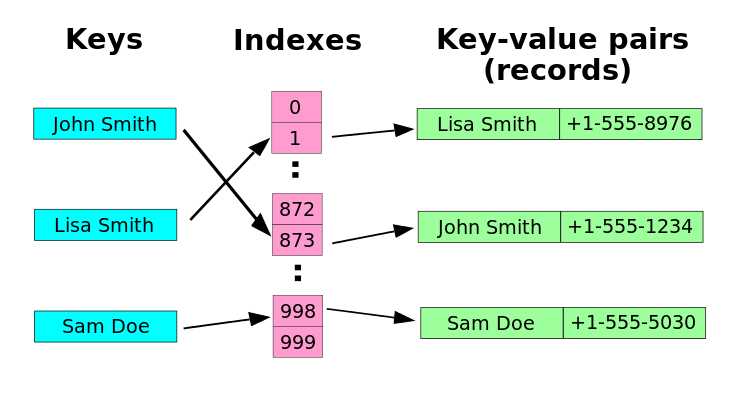
\includegraphics[width=0.7\textwidth]{images/hashmap_wiki.png}}
    \end{center}
    \caption{Un annuaire représenté comme une table de hachage - \cite{ref27}}
    \label{hashmap_wiki}
\end{figure}
Une table de hachage est un tableau associatif. Les composantes de l'association sont la "clé", 
reliée à une ou plusieurs valeurs. Pour insérer, accéder ou supprimer une entrée de la table, 
il faut calculer le "hash" de la clé, \textit{id est} son empreinte unique. Sur la figure \ref{hashmap_wiki}, 
nous apercevons les clés en bleu, le résultat du hash en rouge et les valeurs associées en vert. 
Le risque que deux clés ou plus produisent une même empreinte s'appelle une "collision", c'est 
pour cela qu'une bonne implémentation d'une table de hachage doit non seulement utiliser une bonne 
fonction de hachage mais aussi une manière de résoudre les collisions. C'est ainsi que les trois 
opérations ci-dessus peuvent être réalisées, en moyenne, en temps constant (O(1)) et dans le pire 
des cas (si les collisions s'enchainent) en temps linéaire (O(n)). Dans notre cas, l'utilisation 
d'une table de hachage pour stocker la relation entre un tag et ses fichiers est efficace lorsqu'une 
recherche par tags est demandée. De plus, en associant un ensemble de chemins de fichiers, 
des opérations ensemblistes (union, intersection) peuvent être réalisées lorsque une recherche 
impliquant plusieurs tags est effectuée.
\bigbreak
L'arbre, au sens informatique, est une représentation de la hiérarchie du \acrshort{fs} dans 
notre cas. Prenons comme exemple la hiérarchie suivante :
\dirtree{%
.1 home.
.2 root.
.2 user.
.3 docs.
.4 graph.pdf.
.4 report.tex.
.3 images.
.4 img1.png.
.4 img2.png.
.3 music.
.4 kiss.mp3.
}
Elle peut être obtenue grâce à la commande \mintinline{bash}{tree} sous Linux par exemple.
La même représentation sous forme d'un arbre est illustrée sur la figure \ref{tree} :
\begin{figure}
    \begin{center}
        \fbox{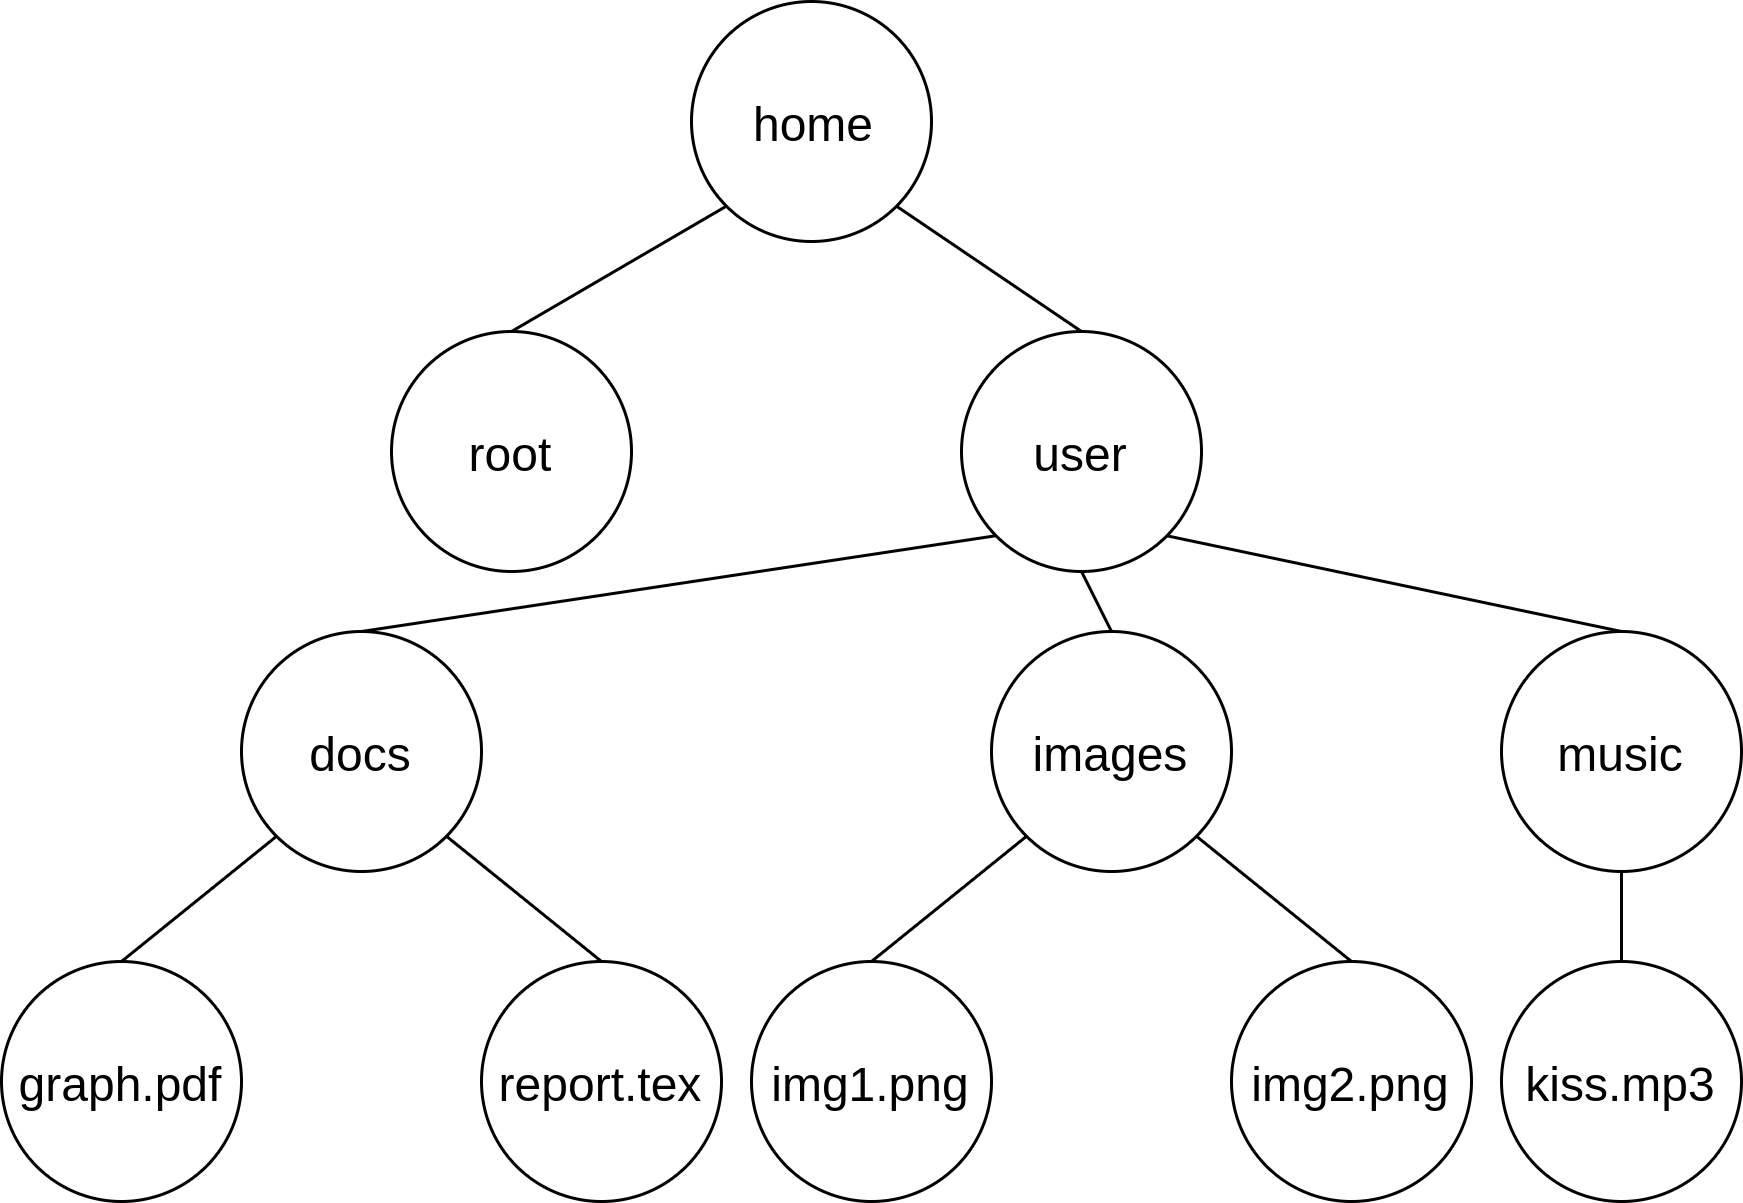
\includegraphics[width=0.8\textwidth]{images/tree.png}}
    \end{center}
    \caption{Représentation sous forme d'arbre d'une hiérarchie de fichiers et répertoires}
    \label{tree}
\end{figure}
Le noeud "home" représente la racine de l'arbre. Chaque noeud représente soit un fichier (en orange), soit 
un répertoire (en bleu) sur le disque. Chaque répertoire peut être vu comme un sous-arbre de l'arbre principal.
Du point de vue programmatoire, un noeud serait défini, au minimum, comme une structure de données 
contenant un champ "données" (dans notre cas, le nom du fichier/répertoire et l'ensemble de ses tags) 
et un champ "enfants", une liste ou un ensemble de pointeurs vers les noeuds enfants. Dans le cas 
présent, seuls les noeuds répertoires pointent vers des noeuds répertoires ou fichiers enfants, 
les fichiers n'auraient qu'une liste vide de pointeurs.
\bigbreak
La table \ref{table_architecture_1} donne, pour chaque événement survenu sur le \acrshort{fs}, les opérations 
à exécuter pour les deux structures de données (la table de hachage et l'arbre) et une approximation 
de la complexité. Les événements sont représentés par leurs numéros, en table 
\ref{table_evenements_possibles}. Les variables suivantes sont définies :
\begin{itemize}
    \item c = Opération constante.
    \item p = Profondeur de l'arbre.
    \item t = Nombre de tags.
\end{itemize}
\begin{center}
    \begin{tabularx}{16cm}{|c|p{6cm}|X|} \hline
        \textbf{Numéro} & \textbf{Opérations sur la \textit{hashmap}} & \textbf{Opérations sur l'arbre} \\ \hline
        1 & Si tag non présent, ajouter le tag comme clé et 
            ajouter le chemin du fichier à l'ensemble -> $O(c)$ & Parcourir l'arbre à la recherche 
            du fichier et ajouter le tag à l'ensemble des tags existants -> $O(p * c)$ \\ \hline
        2 & Supprimer le fichier de l'ensemble des 
            chemins de fichiers associés au tag -> $O(c)$ & Parcourir l'arbre à la recherche 
            du fichier et supprimer le tag de l'ensemble des tags existants -> $O(p * c)$ \\ \hline
        3 & Supprimer la clé et réinsérer la nouvelle clé et l'ensemble associé -> $O(c)$ & Pour l'ensemble 
            des chemins récupérés avec la \textit{hashmap}, modifier les noeuds correspondants -> $O(t * c)$ \\ \hline
        4 & Pour tous les tags du fichier, ajouter au besoin le tag et lui 
            associer le chemin de fichier -> $O(t * c)$ & Parcourir l'arbre à 
            la recherche du répertoire parent du fichier, ajouter le nouveau noeud et l'ensemble 
            de ses tags -> $O(p * c)$ \\ \hline
        5 & Identique à la ligne précédente & Parcourir l'arbre à 
            la recherche du répertoire parent, ajouter le nouveau noeud et l'ensemble 
            de ses tags, puis, récursivement, ajouter ses enfants (sous-répertoires et fichiers) 
            -> $\approx O(p^2 * c)$ \\ \hline
        6 & Pour tous les tags du fichier, associer le nouveau 
            chemin de fichier -> $O(t * c)$ & Parcourir l'arbre à la recherche du parent et 
            changement du lien du noeud avec son parent / simple renommage du nom dans 
            l'étiquette -> $O(p * c)$ \\ \hline
        7 & Pour tous les tags de tous les 
            sous-répertoires et fichiers, associer le nouveau chemin de fichier -> $O(t * p * c)$ 
            & Identique à la ligne précédente \\ \hline
        8 & Pour tous les tags du fichier, supprimer le chemin de fichier 
            -> $O(t * c)$ & Parcourir l'arbre à la recherche du parent et suppression du lien et 
            du noeud -> $O(p * c)$ \\ \hline
        9 & Pour tous les tags de tous les sous-répertoires et fichiers, 
            supprimer le chemin de fichier -> $O(t * p * c)$ & Parcourir l'arbre à la recherche du 
            répertoire parent, supprimer le noeud, l'ensemble de ses tags, et récursivement, ses 
            enfants (sous-répertoires et fichiers) -> $\approx O(p^2 * c)$ \\ \hline
    \end{tabularx}
    \captionof{table}{Opérations et complexité, première architecture}
    \label{table_architecture_1}
\end{center}

Cette version a été en partie abandonnée et adaptée pour deux raisons majeures :
\begin{enumerate}
    \item Avoir deux structures de données interdépendantes augmente la complexité des 
        opérations de mise à jour (ajout, déplacement, suppression de fichiers et tags).
    \item L'implémentation s'est avérée plus difficile que prévue, du fait de certaines 
        contraintes de Rust (voir section \ref{problemes}).
\end{enumerate}

%%%%%%%%%%%%%%%%%%%%%%%%%%%%%%%%%%%%%%%%%%%%%%%%%%%%%%%%%%%%%%%%%%%%%%%%%%%%%%%%%%%%%%%%%%%%%%%%%%%
%%%%%%%%%%%%%%%%%%%%%%%%%%%%%%%%%%%%%%%%%%%%%%%%%%%%%%%%%%%%%%%%%%%%%%%%%%%%%%%%%%%%%%%%%%%%%%%%%%%
\subsubsection{Indexation avec un graphe et une table de hachage}\label{graphe_architecture}
Pendant l'implémentation de cette partie du programme (voir section \ref{problemes}), 
une nouvelle architecture a été imaginée. Elle reprend les bases de la précédente, mais simplifie 
la structure de données. Plutôt que de maintenir deux structures différentes, cette solution 
propose une structure de données principale, secondée par une structure secondaire, optionnelle, 
mais néanmoins efficace :
\begin{enumerate}
    \item Un graphe, avec un noeud représentant soit un répertoire, soit un fichier 
        soit un tag. Chaque noeud est une structure de données comportant un nom et type et est 
        identifié de manière unique. Grâce à cet identifiant, les noeuds sont facilement accessibles.
    \item Une table de hachage, associant le nom d'un tag à son identifiant unique en tant que 
        noeud du graphe.
\end{enumerate}
Un graphe représente un réseau de noeuds qui peuvent être reliés les uns aux autres. Jean-François Hêche, 
professeur à la heig-vd, donne les définitions des graphes non orientés et orientés dans son cours 
sur les "Graphes et Réseaux". Commençons par définir ce qu'est un graphe non orienté : 
"Un graphe non orienté est une structure formée d'un ensemble V, dont les éléments sont appelés les sommets 
ou les noeuds du graphe, et d'un ensemble E, dont les éléments sont appelés les arêtes du graphe, 
et telle qu'à chaque arête est associée une paire de sommets de V appelés les extrémités de 
l'arête." (Hêche, page 1, \cite{ref28}). La figure \ref{graph_undirected} montre un exemple d'un tel 
graphe. 
\begin{figure}
    \begin{center}
        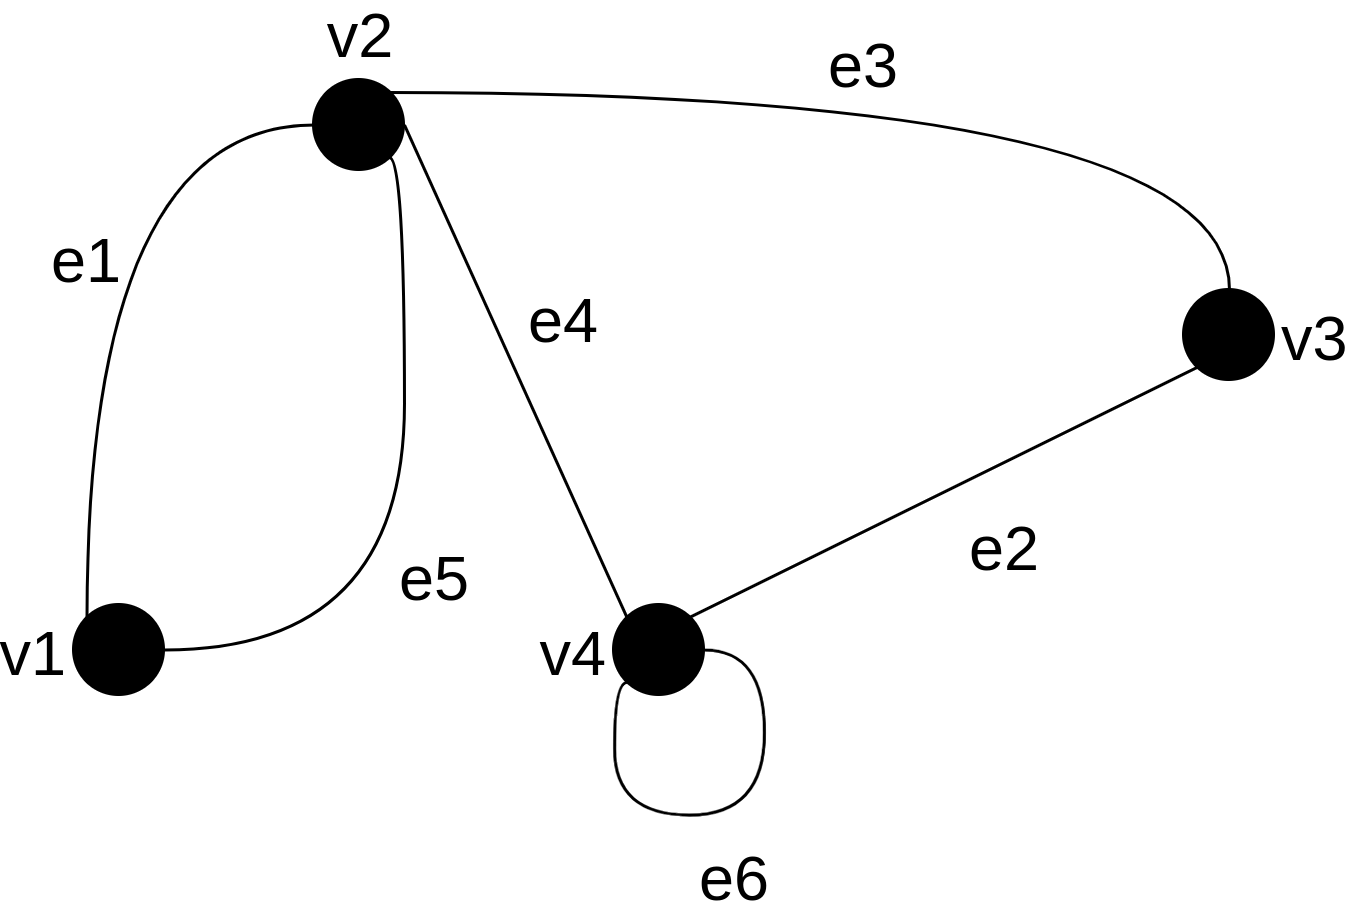
\includegraphics[width=0.8\textwidth]{images/graph_undirected.png}
    \end{center}
    \caption{Graphe non orienté}
    \label{graph_undirected}
\end{figure}
Un graphe orienté est semblable à un graphe non-orienté. La seule différence est qu'une direction 
est donnée au lien entre deux noeuds et ce lien ne se nomme plus "arête" mais "arc". La figure 
\ref{graph_directed} montre un exemple d'un tel graphe.
\begin{figure}
    \begin{center}
        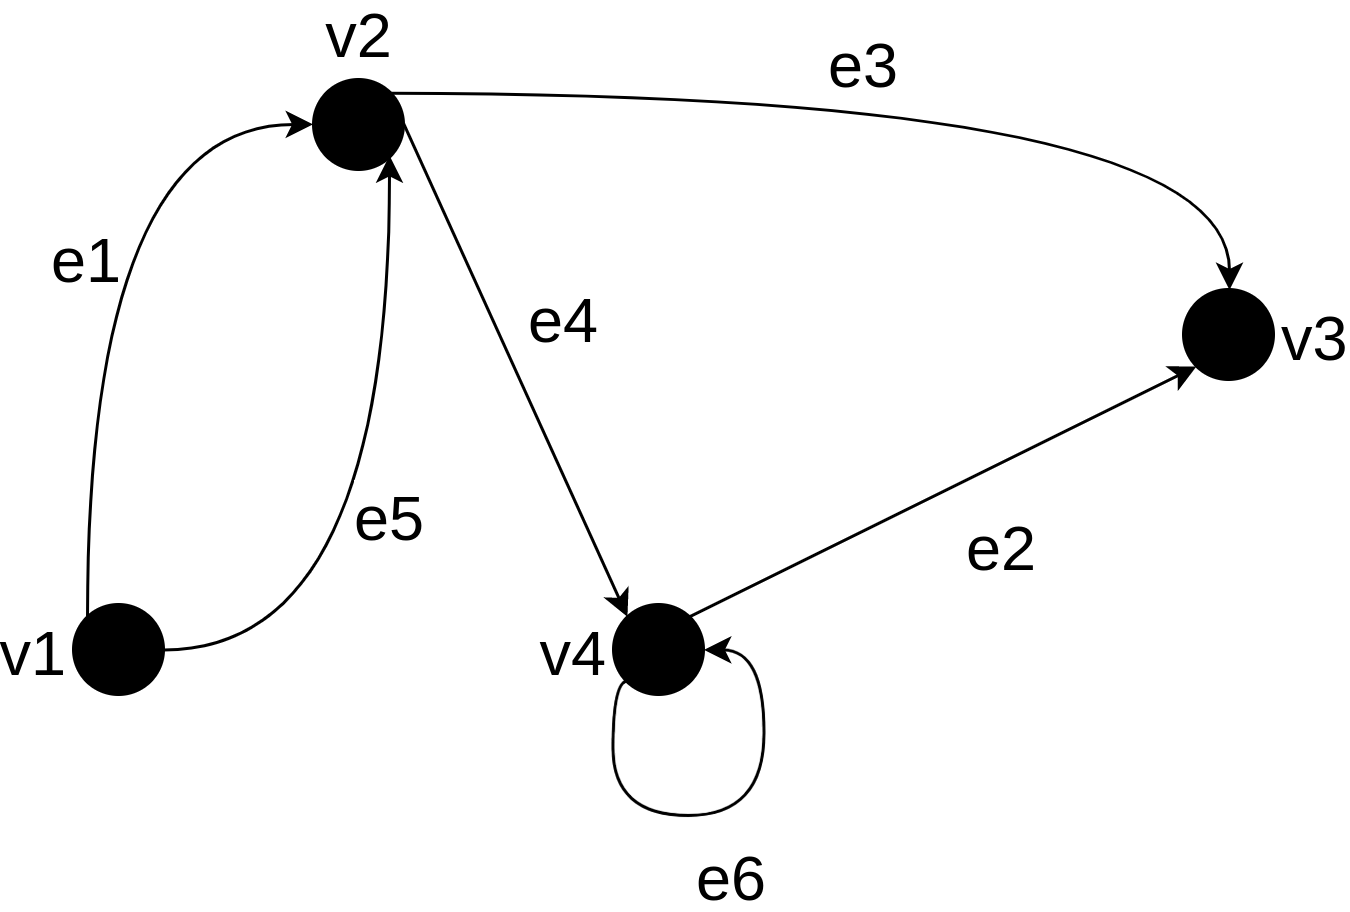
\includegraphics[width=0.8\textwidth]{images/graph_directed.png}
    \end{center}
    \caption{Graphe orienté}
    \label{graph_directed}
\end{figure}
Un graphe est donc un ensemble de noeuds reliés par des arêtes ou des arcs, selon si le graphe est 
orienté ou non. Dans notre cas, l'utilisation d'un graphe n'est pas si éloignée de celle d'un arbre. 
Par ailleurs, selon la théorie des graphes, "un arbre est un graphe sans cycle et connexe" (Hêche, 
page 33, \cite{ref28}). "Sans cycle" signifie qu'un parcours du graphe est possible de telle sorte 
à ce que le noeud de départ et d'arrivée soient différents. "Connexe" définit un graphe tel que 
pour chaque paire de noeuds du graphe il existe un chemin les reliant. L'utilisation d'un tel 
graphe représente fidèlement l'arborescence du \acrshort{fs} (on garde le schéma d'un arbre) 
et simplifie grandement les opérations lorsque des événements surviennent sur ce dernier. 
Le fait d'ajouter les tags comme noeuds du graphe 
maintient une unique structure de données cohérente et diminue le nombre d'opérations différentes 
nécessaires lors de la mise à jour du \acrshort{fs}. Le parcours de ce graphe se fait en 
fonction du chemin de fichier donné, en gardant l'identifiant unique du noeud correspondant au 
répertoire racine, le parcours se fait de la racine vers le noeud final du chemin de fichier.
\bigbreak
La table de hachage utilisée dans cette version peut être vue comme un "cache" d'accès aux noeuds 
tags. En effet, nous pourrions nous passer de cette table de hachage et lorsqu'un accès à un tag 
est demandé, rechercher dans tout le graphe le tag en question. Cependant, cette dernière opération 
devient rapidement conséquente lorsque le graphe comporte de très nombreux noeuds. De plus, cette 
\textit{hashmap} est accédée bien moins souvent que dans la première version de l'architecture, 
car elle est mise à jour uniquement lors des opérations sur les tags et non plus sur celles liées 
seulement aux fichiers et répertoires (opérations potentiellement plus lourdes).
\bigbreak
Comme pour la sous-section \ref{indexation_hashmap_arbre}, la table \ref{table_architecture_2} 
donne pour chaque événement survenu sur le \acrshort{fs}, les opérations 
à exécuter pour les deux structures de données (le graphe et la table de hachage) et une approximation 
de la complexité. Les événements sont représentés par leurs numéros, en table 
\ref{table_evenements_possibles}. Les variables suivantes sont définies :
\begin{itemize}
    \item c = Opération constante.
    \item p = Profondeur du graphe.
    \item t = Nombre de tags.
\end{itemize}
Nous pouvons constater que les opérations sur la table de hachage sont peu nombreuses et souvent 
facultatives, ce qui se traduit par un gain sur le nombre d'opérations totales.
\begin{center}
    \begin{tabularx}{16cm}{|c|X|p{5.5cm}|} \hline
        \textbf{Numéro} & \textbf{Opération graphe} & \textbf{Opération \textit{hashmap}} \\ \hline
        1 & Parcourir le graphe à la recherche du fichier, 
            si besoin créer le noeud tag, et relier le noeud fichier au noeud tag -> $O(p * c)$ 
            & Si non existant, ajouter le nom du tag comme clé et son identifiant dans le graphe 
            comme valeur -> $O(c)$ \\ \hline
        2 & Parcourir le graphe à la recherche du 
            noeud fichier et supprimer le lien entre noeud tag et fichier. Si le noeud tag 
            n'est relié à aucun autre noeud, le supprimer -> $O(p * c)$ & Si le noeud tag 
            n'est relié à aucun autre noeud, supprimer l'entrée -> $O(c)$ \\ \hline
        3 & Obtenir l'identifiant grâce à la hashmap et renommer le noeud correspondant -> $O(c)$ & 
            Supprimer l'entrée et en recréer une avec le nouveau nom et le même identifiant -> $O(c)$ \\ \hline
        4 & Parcourir le graphe à la recherche du répertoire parent, 
            ajouter le nouveau noeud. Pour les tags existants, lier le nouveau noeud, sinon créer 
            le nouveau noeud tag correspondant -> $O(p * t * c)$ & Pour chaque tag, opération identique 
            au numéro 1 \\ \hline
        5 & Parcourir le graphe à la recherche du répertoire parent, 
            ajouter le nouveau noeud. Pour les tags existants, lier le nouveau noeud, sinon créer 
            le nouveau noeud tag correspondant. Répéter pour la sous-arborescence -> $\approx 
            O(p^2 * t * c)$ & Pour chaque tag, opération identique au numéro 1 \\ \hline
        6 & Parcourir le graphe à la recherche du parent et 
            changer le lien du noeud avec son parent / simple renommage du nom dans 
            l'étiquette -> $O(p * c)$ & Pas d'opération requise \\ \hline
        7 & Identique au numéro 6 & Pas d'opération requise \\ \hline
        8 & Parcourir le graphe à la recherche du noeud fichier et supprimer les 
            liens entre noeuds tags et noeud parent -> $O(p * t * c)$ & Pour chaque tag du fichier, 
            supprimer le noeud tag s'il n'a plus de liens vers d'autres noeuds -> $O(t * c)$ \\ \hline
        9 & Parcourir le graphe à la recherche du noeud répertoire et supprimer les 
            liens entre noeuds tags et noeud parent. Répéter pour la sous-arborescence -> $\approx 
            O(p^2 * t * c)$ & Pour chaque sous répertoire ou sous fichier, opération identique au numéro 8 \\ \hline
    \end{tabularx}
    \captionof{table}{Opérations et complexité, deuxième architecture}
    \label{table_architecture_2}
\end{center}

%%%%%%%%%%%%%%%%%%%%%%%%%%%%%%%%%%%%%%%%%%%%%%%%%%%%%%%%%%%%%%%%%%%%%%%%%%%%%%%%%%%%%%%%%%%%%%%%%%%
%%%%%%%%%%%%%%%%%%%%%%%%%%%%%%%%%%%%%%%%%%%%%%%%%%%%%%%%%%%%%%%%%%%%%%%%%%%%%%%%%%%%%%%%%%%%%%%%%%%
\subsection{Surveillance du \acrshort{fs}}
La surveillance du \acrshort{fs} et des tags associés est le deuxième pilier du système. 
L'indexation initiale est nécessaire, mais il est également nécessaire de surveiller en permanence 
l'arborescence des fichiers pour garder cet index à jour. Pour y parvenir, nous allons utiliser 
\mintinline{c}{inotify} (voir section \ref{inotify_techno}), en surveillant tout particulièrement les événements 
suivants :
\begin{itemize}
    \item IN\_ATTRIB : changement sur les tags (ajout, suppression, renommage).
    \item IN\_CREATE : création de fichier/répertoire dans le répertoire surveillé. Ajouter une nouvelle surveillance si répertoire.
    \item IN\_DELETE : suppression d'un fichier/répertoire dans le répertoire surveillé.
    \item IN\_DELETE\_SELF : suppression du répertoire surveillé.
    \item IN\_MOVE\_SELF : suppression d'un fichier/répertoire dans le répertoire surveillé.
    \item IN\_MOVE\_FROM : déplacement/renommage du répertoire (ancien nom).
    \item IN\_MOVE\_TO : déplacement/renommage du répertoire (nouveau nom).
\end{itemize}
Un thread s'occupe d'écouter les événements du \acrshort{fs} et les inscrit dans un buffer 
tandis qu'un autre va mettre à jour le graphe pour répercuter les changements survenus en lisant 
dans ce même buffer (simple pattern producteur-consommateur).

%%%%%%%%%%%%%%%%%%%%%%%%%%%%%%%%%%%%%%%%%%%%%%%%%%%%%%%%%%%%%%%%%%%%%%%%%%%%%%%%%%%%%%%%%%%%%%%%%%%
%%%%%%%%%%%%%%%%%%%%%%%%%%%%%%%%%%%%%%%%%%%%%%%%%%%%%%%%%%%%%%%%%%%%%%%%%%%%%%%%%%%%%%%%%%%%%%%%%%%
\subsection{Requêtes de tags et fichiers}
Une fois que la surveillance du \acrshort{fs} est en place, le système doit pouvoir répondre 
à des requêtes de la part de l'utilisateur. À travers un outil en ligne de commande, l'utilisateur 
a la possibilité de : 
\begin{itemize}
    \item Demander la liste des fichiers et répertoires associés à un ou plusieurs tags. La requête 
        peut être sous la forme d'une expression logique simple (avec les opérateurs logiques "et" 
        et "ou").
    \item Demander la liste des tags déjà existants. 
    \item Renommer un tag. 
\end{itemize}
Pour échanger les requêtes et les réponses, client et serveur communiquent par sockets, avec un 
format de protocole très simple pour distinguer le type d'une requête.

\newpage

\section{Analyse technologique} %-----------------------------------------------------------------------------------------------
%%%%%%%%%%%%%%%%%%%%%%%%%%%%%%%%%%%%%%%%%%%%%%%%%%%%%%%%%%%%%%%%%%%%%%%%%%%%%%%%%%%%%%%%%%%%%%%%%%%
%%%%%%%%%%%%%%%%%%%%%%%%%%%%%%%%%%%%%%%%%%%%%%%%%%%%%%%%%%%%%%%%%%%%%%%%%%%%%%%%%%%%%%%%%%%%%%%%%%%
\subsection{Rust}
Cette section présente le langage de programmation Rust et certains de ses mécanismes, à 
travers quelques exemples, qui sont soit absolument nécessaires pour commencer à programmer avec 
Rust, soit utilisés dans le code de ce projet. Rust est un langage multi paradigmes, fortement typé, 
compilé et performant. Il peut être utilisé en autres pour de la programmation orientée système, 
pour créer des programmes en ligne de commande (\acrshort{cli}) ou pour créer des applications web. 
Fort d'une communauté active, de 
nombreux packages et modules sont disponibles sur \href{https://crates.io}{Crates.io} \cite{ref33} 
et de nombreuses discussions sont présentes sur le \href{https://www.reddit.com/r/rust/}{reddit} 
\cite{ref34} dédié. Pour plus de détails, l'excellent livre \cite{ref0} réalisé par les mainteneurs 
de Rust saura donner de plus amples et précises informations au lecteur avide de connaissances sur 
Rust. Un autre livre \cite{ref2}, plus spécialisé, guide le débutant à Rust dans la conception de 
listes chaînées, car non triviales en Rust de par le fait de ses contraintes.

%%%%%%%%%%%%%%%%%%%%%%%%%%%%%%%%%%%%%%%%%%%%%%%%%%%%%%%%%%%%%%%%%%%%%%%%%%%%%%%%%%%%%%%%%%%%%%%%%%%
%%%%%%%%%%%%%%%%%%%%%%%%%%%%%%%%%%%%%%%%%%%%%%%%%%%%%%%%%%%%%%%%%%%%%%%%%%%%%%%%%%%%%%%%%%%%%%%%%%%
\subsubsection{Installation}
L'installation de Rust sur Linux et macOS est très simple. Les prérequis sont un 
compilateur C (certaines librairies Rust en nécessitent un) et l'outil de transfert de données 
\mintinline{bash}{curl}. Il suffit ensuite d'ouvrir un terminal et d'entrer la commande suivante :
\bigbreak
\begin{code}
    \begin{minted}[bgcolor=mygray,breaklines,breaksymbol=,linenos,frame=single,stepnumber=1,tabsize=2]{bash}
$ curl https://sh.rustup.rs -sSf | sh
    \end{minted}
    \caption{Installation de Rust sur Linux ou macOS}
\end{code}
\bigbreak
Sur Windows, la procédure est un peu plus longue mais tout aussi simple, il faut s'assurer d'avoir 
les C++ build tools pour Visual Studio 2013 ou supérieur. Rust installe son compilateur, 
\mintinline{bash}{rustc}, qui permet de compiler un fichier source (\mintinline{text}{.rs}) en 
fichier exécutable. Nous n'allons cependant pas en parler davantage, la compilation se fera avec 
le gestionnaire de paquets et de compilation Cargo (voir sous-section \ref{cargo_crates}).
Pour plus de détails, se référer au chapitre 1.1 du \textit{book} \cite{ref0}.
Le site \href{https://areweideyet.com/}{Are we (I)DE yet?} \cite{ref1} donne un aperçu des éditeurs 
de texte compatibles avec la chaîne de développement Rust. En ce qui concerne le projet de bachelor 
présenté ici, tout le code a été écrit avec Visual Studio Code.

%%%%%%%%%%%%%%%%%%%%%%%%%%%%%%%%%%%%%%%%%%%%%%%%%%%%%%%%%%%%%%%%%%%%%%%%%%%%%%%%%%%%%%%%%%%%%%%%%%%
%%%%%%%%%%%%%%%%%%%%%%%%%%%%%%%%%%%%%%%%%%%%%%%%%%%%%%%%%%%%%%%%%%%%%%%%%%%%%%%%%%%%%%%%%%%%%%%%%%%
\subsubsection{Cargo et Crates.io}\label{cargo_crates}
Cargo est le système de compilation et exécution et le gestionnaire de paquets intégré à Rust.
Depuis le terminal, ses commandes principales permettent de créer un nouveau projet 
(\mintinline{bash}{cargo new myproject}), de le compiler (\mintinline{bash}{cargo build}), de 
l'exécuter (\mintinline{bash}{cargo run}) ou de générer la documentation associée 
(\mintinline{bash}{cargo doc}). Lorsqu'un nouveau projet est créé avec Cargo, un fichier 
\mintinline{text}{Cargo.toml} est généré (à la manière du fichier \mintinline{text}{package.json} 
avec Node.js et npm) avec le contenu minimal suivant :
\bigbreak
\begin{code}
    \begin{minted}[bgcolor=mygray,breaklines,breaksymbol=,linenos,frame=single,stepnumber=1,tabsize=2]{bash}
[package]
name = "myproject"
version = "0.1.0"
authors = ["Firstname Lastname <me@mail.com>"]

[dependencies]
    \end{minted}
    \caption{Contenu du fichier \mintinline{text}{Cargo.toml}}
\end{code}
\bigbreak
La section "package" contient les informations sur le projet en lui-même. La section "dependencies" 
liste les paquets dont dépend notre application, appelés "\textit{crates}" par la communauté Rust. 
Des milliers de \textit{crates} sont disponibles sur \href{https://crates.io}{Crates.io} \cite{ref33}. 
D'autres sections peuvent être ajoutées au fichier \mintinline{text}{Cargo.toml} pour personnaliser 
les commandes de compilation, créer des workspaces à partir de plusieurs \textit{crates} ou ajouter 
des commandes spécifiques par exemple.
Un sous-chapitre (1.3) et un chapitre entier (14) sont dédiés à Cargo dans le livre de Rust \cite{ref0} 
et il dispose également d'une \href{https://doc.rust-lang.org/cargo/}{documentation complète} 
\cite{ref35} (comme le \textit{book} dédié à Rust).

%%%%%%%%%%%%%%%%%%%%%%%%%%%%%%%%%%%%%%%%%%%%%%%%%%%%%%%%%%%%%%%%%%%%%%%%%%%%%%%%%%%%%%%%%%%%%%%%%%%
%%%%%%%%%%%%%%%%%%%%%%%%%%%%%%%%%%%%%%%%%%%%%%%%%%%%%%%%%%%%%%%%%%%%%%%%%%%%%%%%%%%%%%%%%%%%%%%%%%%
\subsubsection{Généralités}

\paragraph{Commentaires}
Tout texte écrit après deux slashs consécutifs "//" est considéré comme un commentaire en Rust.
La syntaxe multiligne qui existe en C par exemple n'est pas prise en compte. En mettant trois slashs 
consécutifs "///", le commentateur indique au compilateur que ce commentaire fait partie de la 
documentation (qui peut être générée avec Cargo, voir sous-section \ref{cargo_crates}).

\paragraph{Variables}
Tout d'abord, pour déclarer une variable en Rust, il faut utiliser le mot-clé \mintinline{rust}{let}. Une variable 
est par défaut déclarée immutable, \textit{id est} qu'elle ne peut pas être modifiée dans la suite du 
code. Bien que Rust soit un langage fortement typé, son compilateur sait dans la plupart des cas 
inférer le bon type de la variable, soit en analysant la valeur attribuée, soit en analysant la 
première utilisation de la variable (arguments d'une fonction, insertion de données dans le cas 
des collections). Il existe toutefois la possibilité de déclarer explicitement le type de la variable 
en l'indiquant avant le "=". Pour déclarer une variable mutable, il faut lui ajouter le mot-clé 
\mintinline{rust}{mut} avant son nom. Ensuite, les constantes sont déclarées avec le mot-clé \mintinline{rust}{const} 
et leur type doit obligatoirement être indiqué. La différence principale entre les constantes et 
les variables immutables est qu'une constante ne peut être le résultat d'une valeur calculée à 
l'exécution du programme. Enfin, une variable peut être "masquée" ou "obscurcie" (\textit{shadowed}) : 
une nouvelle déclaration avec \mintinline{rust}{let} et le même nom écrase la précédente valeur et 
peut être de type différent. Le listing \ref{rust_variables} montre quelques cas de déclarations de variables :
\bigbreak
\begin{code}
    \begin{minted}[bgcolor=mygray,breaklines,breaksymbol=,linenos,frame=single,stepnumber=1,tabsize=2]{rust}
// Déclaration d'une variable "x", immutable et de type inféré i32
let x = 3;
// Déclaration d'une variable "y", mutable et de type inféré bool
let mut y = true;
// Déclaration d'une variable "z", mutable et de type déclaré char
let mut z : char = 'A';
// La constante PI de type flottant 64 bits
const PI : f64 = 3.1415;
// Shadowing. La première déclaration crée une variable nommée "answer"
// de type i32 et de valeur 42, alors que la deuxième écrase la 
// précédente variable en lui prenant son nom et est de type String.
let answer = 42;
let answer = answer.to_string();
    \end{minted}
    \caption{Exemples de déclarations de variables en Rust}
    \label{rust_variables}
\end{code}
\bigbreak
Pour plus de détails, se référer au chapitre 3.1 du \textit{book} \cite{ref0}.

\paragraph{Types}\label{rust_types}
Il existe deux familles de types en Rust : 
\begin{itemize}
    \item Les scalaires : nombres entiers, nombres à virgule, booleans et caractères.
    \item Les composés (deux types primitifs) : les tuples et les tableaux.
\end{itemize}
Les entiers peuvent être signés ou non signés et sur 8, 16, 32, 64 bits ou dépendant de l'architecture
du processeur (\mintinline{rust}{i8, u8, i16, u16, i32, u32, i64, u64, isize, usize}). Les nombres 
à virgule ont deux possibilités, soit sur 32 bits, soit sur 64 bits (\mintinline{rust}{f32} ou 
\mintinline{rust}{f64}). Le type \mintinline{rust}{bool}, classique, peut prendre deux valeurs, \mintinline{rust}{true} 
ou \mintinline{rust}{false}. Enfin, dernier type primitif scalaire, \mintinline{rust}{char}, stocke 
un caractère Unicode entre simples guillemets. Le premier type primitif composé est le tuple. C'est 
un regroupement de plusieurs valeurs qui peuvent être de différents types. Lors des déclarations, 
les noms de variables, les types et les valeurs d'un tuple sont contenues entre parenthèses et 
séparées par des virgules. Enfin, le type tableau, ou \textit{array} : classique type regroupant 
plusieurs valeurs du même type cette fois. Un \textit{array} a une taille fixe, déterminée à la 
compilation. La déclaration des valeurs d'un tableau se fait entre crochets "[ ]". Pour accéder à une 
valeur du tableau, il faut utiliser la syntaxe \mintinline{rust}{array[i]} où \mintinline{rust}{i} 
est un indice valide du tableau (entre zéro compris et la taille du tableau non compris). Quelques 
exemples sont donnés dans le listing \ref{rust_types_ex}.
\bigbreak
\begin{code}
    \begin{minted}[bgcolor=mygray,breaklines,breaksymbol=,linenos,frame=single,stepnumber=1,tabsize=2]{rust}
let myint : i32 = 1234;
let mychar : char = 'a';
let myfloat : f64 = 2.0;
// Déclaration d'un tuple
let tuple : (char, u32, f64) = ('c', 42, 2.8);
// Destructuration du tuple en trois variables distinctes
let (letter, age, score) = tuple;
// Déclaration d'un tableau
let myarray = ['a', 'b', 'c', 'd', 'e', 'f'];
let x = myarray[4]; // x vaut 'e'
    \end{minted}
    \caption{Quelques types primitifs de Rust}
    \label{rust_types_ex}
\end{code}
\bigbreak
Pour plus de détails, se référer au chapitre 3.2 du \textit{book} \cite{ref0}.

\paragraph{Fonctions}
Comme en C, tout programme a comme point d'entrée la fonction \mintinline{rust}{main()}. Une 
déclaration de fonction commence par le mot-clé \mintinline{rust}{fn}, est suivi du nom de la 
fonction, de la liste des éventuels paramètres et des éventuels types de retour. Lorsqu'une 
fonction a une valeur de retour, la dernière ligne de la fonction qui n'a pas de point-virgule 
à sa fin est évaluée comme une expression et est retournée. Le mot-clé \mintinline{rust}{return} 
existe néanmoins si la fonction doit retourner dans des cas bien précis (dans une condition par 
exemple). Les variables déclarées dans la fonction ne sont pas accessibles depuis l'extérieur de la 
fonction. Les arguments de la fonction sont passés par copie par défaut (voir la sous-section 
\ref{rust_ownership_borrowing} pour plus de détails). Le listing suivant donne l'exemple d'une même 
fonction, en deux versions plus ou moins courtes. Ces fonctions attendent deux entiers et retournent 
également un entier.
\bigbreak
\begin{code}
    \begin{minted}[bgcolor=mygray,breaklines,breaksymbol=,linenos,frame=single,stepnumber=1,tabsize=2]{rust}
fn x_plus_y_plus_one(x : i32, y : i32) -> i32 {
    let x_plus_y = x + y;
    x_plus_y + 1
}

fn x_plus_y_plus_one_short(x : i32, y : i32) -> i32 {
    x + y + 1
}
    \end{minted}
    \caption{Exemples de fonctions en Rust}
    \label{rust_functions}
\end{code}
\bigbreak
Pour plus de détails, se référer au chapitre 3.3 du \textit{book} \cite{ref0}.

\paragraph{Structures de contrôle}
Comme tout langage de programmation, Rust possède des structures de contrôle pour gérer les 
conditions et les répétitions (boucles). Il y a le classique \mintinline{rust}{if condition 
{ ... } else if autre_condition { ... } else { ... }} avec une différence notable par rapport à C : 
il est possible d'affecter une variable avec un \mintinline{rust}{if}, comme dans le listing 
\ref{rust_if}. Il n'y a pas de \mintinline{c}{switch ... case} à proprement parler en Rust, 
nous verrons le \mintinline{rust}{match ... case} à la sous-section \ref{rust_enum_pattern_matching}.
En ce qui concerne les boucles, elles sont au nombre de trois : \mintinline{rust}{loop} (boucle 
infinie), \mintinline{rust}{while} (boucle avec condition initiale) et \mintinline{rust}{for}, 
boucle pour traverser les collections par leurs itérateurs principalement (voir sous-section 
\ref{rust_collections}).
\bigbreak
\begin{code}
    \begin{minted}[bgcolor=mygray,breaklines,breaksymbol=,linenos,frame=single,stepnumber=1,tabsize=2]{rust}
// Exemple d'un simple if ... else
let name = "fred";
if name == "fred" {
    println!("Hello buddy !");
}
else {
    println!("Hello World !");
}

// Exemple d'affectation d'une variable avec un if. Ici, n vaudra 42
let condition = true;
let n = if condition { 42 }
else { 66 };
    \end{minted}
    \caption{Exemples de conditions en Rust}
    \label{rust_if}
\end{code}
\bigbreak
\begin{code}
    \begin{minted}[bgcolor=mygray,breaklines,breaksymbol=,linenos,frame=single,stepnumber=1,tabsize=2]{rust}
// Boucle infinie
loop {
    println!("Forever");
}
// Boucle avec condition
let mut x = 0;
while x < 10 {
    println!("{}", x);
    x = x + 1;
}
// Parcours d'un tableau
let myarray = [1, 2, 3, 4, 5];
for elem in myarray.iter() {
    println!("value : {}", elem);
}
    \end{minted}
    \caption{Exemples de boucles en Rust}
    \label{rust_loop}
\end{code}
\bigbreak
Pour plus de détails, se référer au chapitre 3.5 du \textit{book} \cite{ref0}.

\paragraph{Organisation des fichiers et modules}
Un programme écrit en Rust peut être découpé en plusieurs fichiers et modules. 
Un module peut contenir des déclarations de fonctions, de structures et leurs implémentations (voir 
section \ref{rust_struct_data}), etc. Le mot-clé pour déclarer un module est \mintinline{rust}{mod}. 
Le code à l'intérieur du module est par défaut privé, pour le rendre accessible en dehors du module, 
le préfixe \mintinline{rust}{pub} est disponible. Pour utiliser un module au sein d'un autre ou dans 
\mintinline{rust}{main.rs}, il faut l'importer avec le mot-clé \mintinline{rust}{use}. Par défaut, 
tout module est défini dans le fichier \mintinline{text}{src/lib.rs} d'un projet. Si de nombreux 
modules sont déclarés, il est possible de les mentionner dans \mintinline{text}{src/lib.rs} de cette 
manière : \mintinline{rust}{mod mymodule;} et de créer un fichier ayant le même nom que le module 
(dans cet exemple, \mintinline{text}{src/mymodule.rs}) contenant le code en question. Une déclaration 
de module peut en contenir d'autres également, créant ainsi une hiérarchie de modules.
Pour plus de détails, se référer au chapitre 7 du \textit{book} \cite{ref0}.

%%%%%%%%%%%%%%%%%%%%%%%%%%%%%%%%%%%%%%%%%%%%%%%%%%%%%%%%%%%%%%%%%%%%%%%%%%%%%%%%%%%%%%%%%%%%%%%%%%%
%%%%%%%%%%%%%%%%%%%%%%%%%%%%%%%%%%%%%%%%%%%%%%%%%%%%%%%%%%%%%%%%%%%%%%%%%%%%%%%%%%%%%%%%%%%%%%%%%%%
\subsubsection{Structures de données}\label{rust_struct_data}
Comme en C, Rust octroie la possibilité au programmeur de définir ses propres types composés, les 
\mintinline{rust}{struct}. La déclaration et l'instanciation d'une structure se font comme en C 
avec quelques raccourcis disponibles. Une structure sans noms de champs est également disponible, 
appelée "tuple struct". Pour accéder aux champs d'une structure, il suffit d'utiliser la notation 
pointée (\mintinline{rust}{player.name}).
\bigbreak
\begin{code}
    \begin{minted}[bgcolor=mygray,breaklines,breaksymbol=,linenos,frame=single,stepnumber=1,tabsize=2]{rust}
// Structure définissant un personnage dans un jeu vidéo
struct Player {
    name: String,
    class: String,
    life: i32,
    active: bool
}
// Création d'une variable Player
let player_one = Player {
    name: String::from("Groumf"),
    class: String::from("Wizard"),
    life: 100,
    active: true
};

// Structure sans noms aux champs
struct Coordinates(f64, f64);
let geneva = Coordinates(46.2016, 6.146);

// Structure vide ()
struct Nil;
    \end{minted}
    \caption{Exemples de structures en Rust}
    \label{rust_struct}
\end{code}
\bigbreak
La particularité des structures, par rapport à C, est qu'il est possible de définir des méthodes 
rattachées aux structures, à la manière des méthodes en Java, sans pour autant obtenir une classe 
\textit{stricto sensu} des langages orientés objets, même si le résultat final est très semblable.
Pour définir des méthodes à une structure, il est nécessaire de déclarer un bloc de code commençant 
par le mot-clé \mintinline{rust}{impl} suivi du nom de la structure et d'accolades. À l'intérieur 
de ce bloc sont définies des fonctions en relation avec la structure. Dans le listing 
\ref{rust_struct_impl}, nous voyons la déclaration de la structure \mintinline{rust}{Player} et de 
son implémentation, comportant trois méthodes (avec la syntaxe des fonctions) pour créer un nouveau 
personnage, qu'il puisse en attaquer un autre et qu'il puisse saluer. La seule différence entre une 
méthode et une fonction est qu'une méthode qui est appelée sur une variable du type de la structure 
avec la notation pointée attend le paramètre \mintinline{rust}{self} comme premier paramètre, 
obligatoirement. \mintinline{rust}{self} réfère à la variable elle-même, comme \mintinline{java}{this} 
en Java. Nous pouvons voir que \mintinline{rust}{self} et les autres paramètres ont une syntaxe non 
décrite pour l'instant (\mintinline{rust}{&} et \mintinline{rust}{&mut}), la sous-section 
\ref{rust_ownership_borrowing} donne de plus amples explications.
\bigbreak
\begin{code}
    \begin{minted}[bgcolor=mygray,breaklines,breaksymbol=,linenos,frame=single,stepnumber=1,tabsize=2]{rust}
struct Player {
    name: String, class: String, life: i32, force: i32
}

impl Player {
    fn new(name : String, class : String) -> Player {
        Player { name, class, life : 100, force : 10 }
    }

    fn attack(&self, other : &mut Player) {
        other.life = other.life - self.force;
    }

    fn say_hi(&self) {
        println!("Hi, I'm {}, powerfull {} !", self.name, self.class);
    }
}

fn main() {
    let player_one = Player::new(String::from("Groumf"),
        String::from("Wizard"));
    let mut player_two = Player::new(String::from("Trabi"),
        String::from("Bard"));
    player_one.attack(&mut player_two);
    player_one.say_hi();
}
    \end{minted}
    \caption{Bloc \mintinline{rust}{impl} d'une structure en Rust}
    \label{rust_struct_impl}
\end{code}
\bigbreak
Pour plus de détails, se référer au chapitre 5 du \textit{book} \cite{ref0}.

%%%%%%%%%%%%%%%%%%%%%%%%%%%%%%%%%%%%%%%%%%%%%%%%%%%%%%%%%%%%%%%%%%%%%%%%%%%%%%%%%%%%%%%%%%%%%%%%%%%
%%%%%%%%%%%%%%%%%%%%%%%%%%%%%%%%%%%%%%%%%%%%%%%%%%%%%%%%%%%%%%%%%%%%%%%%%%%%%%%%%%%%%%%%%%%%%%%%%%%
\subsubsection{Traits et généricité}\label{trait_generic}
Les traits en Rust sont l'équivalent des interfaces en Java. C'est une manière de définir 
un comportement abstrait que pourrait suivre un type. Le listing \ref{rust_trait} définit 
un trait "véhicule" (\mintinline{rust}{Vehicle}) qu'implémentent les structures "vélo" 
(\mintinline{rust}{Bicycle}) et "avion" (\mintinline{rust}{Plane}). Le trait 
\mintinline{rust}{Vehicle} donne la signature d'une seule fonction, \mintinline{rust}{description()} 
qui décrit la variable du type en question. Les deux structures implémentant le trait doivent également 
implémenter toutes les fonctions du trait.
\bigbreak
\begin{code}
    \begin{minted}[bgcolor=mygray,breaklines,breaksymbol=,linenos,frame=single,stepnumber=1,tabsize=2]{rust}
trait Vehicle { fn description(&self); }

struct Bicycle { wheels : u8, passengers : u8 }
impl Vehicle for Bicycle {
    fn description(&self) {
        println!("I'm a bicycle, I have {} wheels and \
            can carry {} passengers.", 
            self.wheels, self.passengers);
    }
}

struct Plane { engines : u8, passengers : u16, fuel : String }
impl Vehicle for Plane {
    fn description(&self) {
        println!("I'm a plane, I have {} engines and \
            can carry {} passengers. I fly with {}.", 
            self.engines, self.passengers, self.fuel);
    }
}

fn main() {
    let bicycle = Bicycle { wheels : 2, passengers : 1 };
    bicycle.description();
    let plane = Plane { engines : 1, passengers : 100, 
        fuel : String::from("kerosene") };
    plane.description();
}
    \end{minted}
    \caption{Implémentations d'un trait en Rust}
    \label{rust_trait}
\end{code}
\bigbreak
Les traits peuvent être déclarés génériques, comme les fonctions d'ailleurs. La généricité 
n'est pas un concept réservé à Rust, de nombreux langages de programmation l'utilisent. C'est une 
manière d'éviter de répéter un même code pour des types de données différents, mais qui auraient 
des similitudes. Prenons l'exemple d'une fonction faisant l'addition de deux nombres. Les arguments 
pourraient être soit des nombres entiers, soit des nombres à virgule. La méthode pour additionner 
ces deux types est la même. Mais pour un langage fortement typé comme Rust, il est nécessaire de 
définir précisément les types des arguments des fonctions. C'est là qu'entre en jeu la généricité : 
la déclaration d'une fonction attend un type générique, usuellement nommé \mintinline{rust}{T}, 
et le manipule comme un type réel. De nombreux types de la librairie standard sont génériques, 
comme les types \mintinline{rust}{Option} et \mintinline{rust}{Result} (voir sous-section 
\ref{rust_enum_pattern_matching}).
Pour plus de détails, se référer au chapitre 10 du \textit{book} \cite{ref0}.

%%%%%%%%%%%%%%%%%%%%%%%%%%%%%%%%%%%%%%%%%%%%%%%%%%%%%%%%%%%%%%%%%%%%%%%%%%%%%%%%%%%%%%%%%%%%%%%%%%%
%%%%%%%%%%%%%%%%%%%%%%%%%%%%%%%%%%%%%%%%%%%%%%%%%%%%%%%%%%%%%%%%%%%%%%%%%%%%%%%%%%%%%%%%%%%%%%%%%%%
\subsubsection{Énumérations et \textit{pattern matching}}\label{rust_enum_pattern_matching}
Les énumérations sont une autre manière de concevoir ses propres types. Comme en C, une énumération
liste toutes les variantes possibles d'une valeur d'un même type. L'exemple classique d'une énumération 
sont les jours de la semaine. Sept cas différents, sans évolutions possibles. Les énumérations en 
Rust prennent tout leur sens en combinaison avec les \textit{pattern matching} : une structure 
de contrôle ressemblant à un \mintinline{c}{switch ... case} en C mais avec un côté davantage 
emprunté à la programmation fonctionnelle (on les retrouve d'ailleurs en Scala). Tous les cas 
possibles d'une énumération doivent être traité avec un \mintinline{rust}{match} (d'où la clause 
par défaut \mintinline{rust}{_}). Le bloc de code à droite de chaque \mintinline{rust}{=>} peut être 
retourné, comme pour une fonction (voir listing \ref{rust_enum}).
\bigbreak
\begin{code}
    \begin{minted}[bgcolor=mygray,breaklines,breaksymbol=,linenos,frame=single,stepnumber=1,tabsize=2]{rust}
enum Direction {
    North, South, East, West
}

fn print_direction(direction : Direction) {
    match direction {
        Direction::North => println!("Go North"),
        Direction::South => println!("Go South"),
        _ => println!("Go East or West") // clause par défaut
    }
}
    \end{minted}
    \caption{Définition d'une \mintinline{rust}{enum} et son utilisation avec un \textit{pattern matching} en Rust}
    \label{rust_enum}
\end{code}
\bigbreak
Rust possède dans la librairie standard une énumération très puissante : \mintinline{rust}{Option} 
(recopiée dans le listing \ref{rust_option}). Elle remplace le tristement fameux \mintinline{c}{NULL} 
en C ou d'autres langages. Elle supprime simplement d'innombrables bugs souvent rencontrés à cause 
de \mintinline{c}{NULL}. Si une variable existe, elle se retrouve dans le cas \mintinline{rust}{Some} 
de l'option, si elle n'existe pas, dans le cas \mintinline{rust}{None}. Cette énumération est de 
plus générique (voir sous-section \ref{trait_generic}), elle accepte tout type de données.
\bigbreak
\begin{code}
    \begin{minted}[bgcolor=mygray,breaklines,breaksymbol=,linenos,frame=single,stepnumber=1,tabsize=2]{rust}
enum Option<T> {
    Some(T),
    None,
}
fn process(value : Option<u32>) {
    match value {
        Some(data) => println!("{}", data),
        None => println!("Error, no data")
    }
}
    \end{minted}
    \caption{L'énumération \mintinline{rust}{Option} et son utilisation avec un \textit{pattern matching} en Rust}
    \label{rust_option}
\end{code}
\bigbreak
Pour plus de détails, se référer au chapitre 6 du \textit{book} \cite{ref0}.

%%%%%%%%%%%%%%%%%%%%%%%%%%%%%%%%%%%%%%%%%%%%%%%%%%%%%%%%%%%%%%%%%%%%%%%%%%%%%%%%%%%%%%%%%%%%%%%%%%%
%%%%%%%%%%%%%%%%%%%%%%%%%%%%%%%%%%%%%%%%%%%%%%%%%%%%%%%%%%%%%%%%%%%%%%%%%%%%%%%%%%%%%%%%%%%%%%%%%%%
\subsubsection{Collections}\label{rust_collections}
Cette sous-section décrit les deux collections les plus utilisées en Rust, à savoir les vecteurs 
(\mintinline{rust}{Vec}) et les tables de 
hachage associatives (\mintinline{rust}{HashMap}). Un vecteur est un tableau qui n'a pas de taille 
fixe, des éléments peuvent lui être ajoutés ou enlevés. C'est l'équivalent des \mintinline{java}{ArrayList} 
en Java. Un vecteur est générique (voir sous-section \ref{trait_generic}), il peut contenir tout type 
de données, mais un seul type à la fois. 
De nombreuses méthodes existent pour manipuler un vecteur, que ce soit pour lui ajouter ou enlever 
des éléments ou pour le convertir vers d'autre formes. Une macro, \mintinline{rust}{vec!} est 
disponible pour rapidement créer un vecteur (éléments séparés par des virgules entre "[ ]").
Le listing \ref{rust_collections_vec} donne quelques exemples :
\bigbreak
\begin{code}
    \begin{minted}[bgcolor=mygray,breaklines,breaksymbol=,linenos,frame=single,stepnumber=1,tabsize=2]{rust}
// Déclaration d'un vecteur avec new, puis avec la macro
let v: Vec<char> = Vec::new();
let mut v = vec!['a', 'b', 'c'];
// Ajout d'un élément au vecteur
v.push('d');
// Accès au deuxième élément du vecteur, de deux manière différentes
let second: &char = &v[1];
let second: Option<&char> = v.get(1);
// Parcours (immutable) du vecteur avec la syntaxe for .. in ..
for i in &v {
    println!("{}", i);
}
    \end{minted}
    \caption{Exemples de déclarations et utilisations d'un vecteur}
    \label{rust_collections_vec}
\end{code}
\bigbreak
Une \mintinline{rust}{HashMap} est une table de hachage associative, tel qu'il en existe en Java.
Elle est, comme le vecteur, générique (voir sous-section \ref{trait_generic}), elle accepte tout 
type de données. C'est une structure de données efficace pour accéder rapidement à une information.
Le listing \ref{rust_collections_hashmap} donne quelques exemples :
\bigbreak
\begin{code}
    \begin{minted}[bgcolor=mygray,breaklines,breaksymbol=,linenos,frame=single,stepnumber=1,tabsize=2]{rust}
// Déclaration d'une hashmap avec new
let h: HashMap<char, u32> = HashMap::new();
// Ajout d'une paire clé-valeur à la hashmap
h.insert('a', 97);
// Accès à la valeur associée à la clé 'a', retourne une Option
let a: Option<&u32> = h.get('a');
// Parcours (immutable) de la hashmap avec la syntaxe for .. in ..
for (key, value) in &h {
    println!("{}: {}", key, value);
}
    \end{minted}
    \caption{Exemples de déclaration et utilisation d'une \mintinline{rust}{HashMap}}
    \label{rust_collections_hashmap}
\end{code}
\bigbreak
Pour plus de détails, se référer au chapitre 8 du \textit{book} \cite{ref0}.

%%%%%%%%%%%%%%%%%%%%%%%%%%%%%%%%%%%%%%%%%%%%%%%%%%%%%%%%%%%%%%%%%%%%%%%%%%%%%%%%%%%%%%%%%%%%%%%%%%%
%%%%%%%%%%%%%%%%%%%%%%%%%%%%%%%%%%%%%%%%%%%%%%%%%%%%%%%%%%%%%%%%%%%%%%%%%%%%%%%%%%%%%%%%%%%%%%%%%%%
\subsubsection{\textit{Ownership}, \textit{Borrowing} et références}\label{rust_ownership_borrowing}
La caractéristique unique de Rust est sans aucun doute l'\textit{ownership}, ou "possession". 
L'\textit{ownership} est défini par ces trois règles :
\begin{itemize}
    \item Chaque variable est dite le "possesseur" (\textit{owner}) d'une valeur.
    \item Il ne peut y avoir qu'un seul \textit{owner} pour une valeur.
    \item Lorsque l'\textit{owner} est détruit ou change de portée, la valeur est détruite.
\end{itemize}
Avant de continuer sur cette notion, un bref rappel sur l'utilisation de la mémoire est nécessaire. 
Le système d'exploitation (\acrshort{os}) met à disposition d'un programme deux zones mémoire différentes pour stocker ses 
variables : la pile (\textit{stack}) et le tas (\textit{heap}). Le mécanisme d'accès à la pile est 
simple et rapide et stocke des variables dont la taille est fixe et connue à la compilation. Les 
variables de type primitifs (voir paragraphe \ref{rust_types}) sont stockées dans la pile. Lorsqu'une 
variable dont la taille n'est pas connue à l'avance (type évolué, par exemple les collections) est 
déclarée, elle placée dans le tas. Un programme voulant stocker une variable sur le tas est obligé 
de demander à l'\acrshort{os} de chercher un espace disponible assez grand pour stocker la variable 
et qu'il lui donne un pointeur vers cette zone, pour la retrouver par la suite.
\bigbreak
Lorsqu'une valeur est assignée à une variable, elle est détenue par cette variable jusqu'à sa 
destruction. Le listing \ref{rust_ownership_scope} illustre un exemple :
\bigbreak
\begin{code}
    \begin{minted}[bgcolor=mygray,breaklines,breaksymbol=,linenos,frame=single,stepnumber=1,tabsize=2]{rust}
{
    // my_vec est le "propriétaire" de ce vecteur
    let my_vec = vec![3, 2, 1]; 
    ... // my_vec est utilisé
} // la portée de my_vec se termine ici, my_vec est alors supprimé
    \end{minted}
    \caption{Portée d'une variable en Rust}
    \label{rust_ownership_scope}
\end{code}
\bigbreak
La variable \mintinline{rust}{my_vec} se trouve sur la pile, mais les données vers lesquelles elle 
pointe se trouvent dans le tas. Lorsque \mintinline{rust}{my_vec} sera hors de portée, les données 
dans la pile et dans le tas seront libérées. Si \mintinline{rust}{my_vec} est assigné à une autre 
variable, l'\textit{ownership} des données est transféré à cette nouvelle variable, 
\mintinline{rust}{my_vec} ne sera plus accessible et utilisable après l'affectation, comme illustré
au listing \ref{rust_ownership_transfer}. Ce cas de figure ne se présente pas avec les types primitifs 
dont la taille en mémoire est connue à la compilation et où une copie des données est effectuée. 
Pour qu'un type évolué puisse être copié de cette façon, il doit implémenter le trait \mintinline{rust}{Copy}.
\bigbreak
\begin{code}
    \begin{minted}[bgcolor=mygray,breaklines,breaksymbol=,linenos,frame=single,stepnumber=1,tabsize=2]{rust}
{
    // Ici pas de problèmes, a et b sont de type primitif i32, de
    // taille fixe et connue, la valeur de a est copiée dans b.
    let a = 10;
    let b = a;

    let mut my_vec = vec![3, 2, 1]; 
    let other_vec = my_vec;
    my_vec.push(42); // Erreur, la valeur a été déplacée (move)
}
    \end{minted}
    \caption{Transfert de l'\textit{ownership} en Rust}
    \label{rust_ownership_transfer}
\end{code}
\bigbreak
À la ligne 8 du listing \ref{rust_ownership_transfer}, la variable \mintinline{rust}{my_vec} est 
invalidée, mais pas les données vers lesquelles elle pointe. Il n'y a que le pointeur vers ces données 
qui transféré vers \mintinline{rust}{other_vec}. C'est ici que la deuxième règle de l'\textit{ownership} 
s'applique, il ne peut y avoir plus d'un \textit{owner} d'une même valeur au même moment. 
Pour réaliser une vraie copie des données d'un vecteur à un autre, ou de manière générale pour un 
type évolué, il faut appeler la méthode \mintinline{rust}{clone()}, qui copie entièrement les 
données en mémoire. Cette situation de transfert d'\textit{ownership} survient également lors des 
appels à des fonctions. Si un paramètre est donné à une fonction, la fonction en prend possession, 
comme illustré au listing \ref{rust_ownership_transfer_function}.
\bigbreak
\begin{code}
    \begin{minted}[bgcolor=mygray,breaklines,breaksymbol=,linenos,frame=single,stepnumber=1,tabsize=2]{rust}
fn main() {
    let mut my_vec = vec![3, 2, 1]; 
    print_vec(my_vec); // La fonction prend possession du vecteur
    my_vec.push(42); // Erreur, la valeur a été déplacée (move)
}

fn print_vec(v : Vec<i32>) {
    println!("My super vector : {:?}", v);
}
    \end{minted}
    \caption{Transfert de l'\textit{ownership} vers une fonction en Rust}
    \label{rust_ownership_transfer_function}
\end{code}
\bigbreak
Pour palier à ce problème de transfert de possession lors d'appels aux fonctions, deux solutions existent :
\begin{enumerate}
    \item La fonction doit retourner la valeur possédée. Ce n'est pas pratique si le but de la fonction 
        est de retourner le résultat d'une opération. Elle peut retourner un tuple formé de la ou 
        les valeurs accaparées et du résultat de son opération. Cette manière de faire est lourde 
        et non conseillée.
    \item La fonction peut "emprunter" la variable de différentes manières (voir ci-dessous).
\end{enumerate}
Heureusement, les fonctions peuvent se "prêter" les variables par \textit{borrowing} ("emprunt").
Deux types de références aux variables sont disponibles :
\begin{enumerate}
    \item Les références immutables (syntaxe \mintinline{rust}{&ma_variable}).
    \item Les références mutables (syntaxe \mintinline{rust}{&mut ma_variable}).
\end{enumerate}
Le listing \ref{rust_borrowing} montre un exemple d'emprunt immutable et mutable.
\bigbreak
\begin{code}
    \begin{minted}[bgcolor=mygray,breaklines,breaksymbol=,linenos,frame=single,stepnumber=1,tabsize=2]{rust}
fn main() {
    let mut my_vec = vec![3, 2, 1]; 
    // La fonction emprunte de manière immutable le vecteur
    ref_immutable(&my_vec);
    // La fonction emprunte de manière mutable le vecteur
    ref_mutable(&mut my_vec);
}

fn ref_immutable(v : &Vec<i32>) {
    println!("My super vector : {:?}", v);
}

fn ref_mutable(v : &mut Vec<i32>) {
    v.push(42);
}
    \end{minted}
    \caption{Emprunts de variables entre fonctions en Rust}
    \label{rust_borrowing}
\end{code}
\bigbreak
Ces références sont proches conceptuellement des pointeurs en C (Rust accepte d'ailleurs le 
déréférencement des variables avec le symbole \mintinline{rust}{*}) mais obéissent à deux 
règles fondamentales :
\begin{enumerate}
    \item À tout moment, il peut y avoir soit une seule référence mutable, soit plusieurs 
        références immutables, mais pas les deux en même temps.
    \item Les références doivent toujours être valides.
\end{enumerate}
Grâce aux références, Rust évite les problèmes de concurrence sur les valeurs pointées ainsi que 
les pointeurs invalides. Pour plus de détails, se référer au chapitre 4 du \textit{book} \cite{ref0}.
Il existe également d'autres types de pointeurs, dits "intelligents". Le livre sur Rust dédie un 
chapitre entier à eux (chapitre 15 du \textit{book} \cite{ref0}).

%%%%%%%%%%%%%%%%%%%%%%%%%%%%%%%%%%%%%%%%%%%%%%%%%%%%%%%%%%%%%%%%%%%%%%%%%%%%%%%%%%%%%%%%%%%%%%%%%%%
%%%%%%%%%%%%%%%%%%%%%%%%%%%%%%%%%%%%%%%%%%%%%%%%%%%%%%%%%%%%%%%%%%%%%%%%%%%%%%%%%%%%%%%%%%%%%%%%%%%
\subsubsection{Gestion des erreurs} 
Nonobstant son compilateur très restrictif, détectant à la compilation de nombreuses erreurs, Rust 
a une gestion avancée des erreurs survenant à l'exécution. Il distingue deux types : les erreurs 
récupérables et les erreurs irrécupérables (non pas comme dans les langages comme Java ou le concept 
d'exceptions mélange ces deux types d'erreurs). Pour ces dernières, Rust offre une macro, 
\mintinline{rust}{panic!}, stopant abruptement le programme et affichant un message d'erreur sur 
la sortie standard en indiquant à quelle ligne le programme a planté. Pour les erreurs récupérables, 
une manière plus élégante existe : à la manière de l'énumération \mintinline{rust}{Option} vue à 
la section \ref{rust_enum_pattern_matching}, l'énumération \mintinline{rust}{Result} a été conçue 
pour gérer les erreurs au \textit{runtime} (voir listing \ref{rust_result}).
\bigbreak
\begin{code}
    \begin{minted}[bgcolor=mygray,breaklines,breaksymbol=,linenos,frame=single,stepnumber=1,tabsize=2]{rust}
enum Result<T, E> {
    Ok(T),
    Err(E),
}

fn process(value : Result<u32, std::io::Error>) {
    match value {
        Ok(data) => println!("u32 value : {}", data),
        Err(error) => println!("Error : {}", error)
    }
}
    \end{minted}
    \caption{L'énumération \mintinline{rust}{Result} et son utilisation avec un \textit{pattern matching} en Rust}
    \label{rust_result}
\end{code}
\bigbreak
De nombreuses fonctions de la librairie standard et de la communauté retournent des 
\mintinline{rust}{Result}, notamment lors de l'ouverture d'un fichier. Comme ce genre d'opérations 
sont courantes, Rust met à disposition deux fonctions équivalentes à réaliser un \mintinline{rust}{match} 
sur un \mintinline{rust}{Result}, \mintinline{rust}{unwrap()} et \mintinline{rust}{expect()}. La 
seule différence entre les deux est qu'avec la deuxième fonction, un message personnalisé est 
attendu en argument. Le listing \ref{rust_result_file} montre les différentes façons de traiter un 
\mintinline{rust}{Result} lors de l'ouverture d'un fichier :
\bigbreak
\begin{code}
    \begin{minted}[bgcolor=mygray,breaklines,breaksymbol=,linenos,frame=single,stepnumber=1,tabsize=2]{rust}
fn main() {
    // Version 1
    let f = File::open("test.txt");
    let f = match f {
        Ok(file) => file,
        Err(error) => {
            panic!("Error on opening file : {:?}", error)
        },
    };
    // Version 2
    let f = File::open("test.txt").unwrap();
    // Version 3
    let f = File::open("test.txt").expect("Error on opening test.txt");
}
    \end{minted}
    \caption{Ouverture d'un fichier et son traitement en Rust}
    \label{rust_result_file}
\end{code}
\bigbreak
Pour plus de détails, se référer au chapitre 9 du \textit{book} \cite{ref0}.

%%%%%%%%%%%%%%%%%%%%%%%%%%%%%%%%%%%%%%%%%%%%%%%%%%%%%%%%%%%%%%%%%%%%%%%%%%%%%%%%%%%%%%%%%%%%%%%%%%%
%%%%%%%%%%%%%%%%%%%%%%%%%%%%%%%%%%%%%%%%%%%%%%%%%%%%%%%%%%%%%%%%%%%%%%%%%%%%%%%%%%%%%%%%%%%%%%%%%%%
\subsubsection{Tests}
Lorsqu'un nouveau projet \textit{librairie} est créé avec \mintinline{bash}{cargo new mylib --lib}, 
un module de tests unitaires est \textit{de facto} ajouté au fichier \mintinline{rust}{lib.rs}, 
comme dans le listing \ref{rust_test_module} :
\bigbreak
\begin{code}
    \begin{minted}[bgcolor=mygray,breaklines,breaksymbol=,linenos,frame=single,stepnumber=1,tabsize=2]{rust}
#[cfg(test)]
mod tests {
    #[test]
    fn it_works() {
        assert_eq!(2 + 2, 4);
    }
}
    \end{minted}
    \caption{Module de test ajouté automatiquement}
    \label{rust_test_module}
\end{code}
\bigbreak
Chaque fonction précédée par l'attribut \mintinline{rust}{#[test]} est considérée par le compilateur 
comme un test. Pour exécuter les tests, Cargo met à disposition une commande, \mintinline{bash}{cargo test}. 
Lorsque cette commande est exécutée, tous les tests sont effectués en parallèle, sans garantir un 
ordre d'exécution prédéfini. Un résumé des tests effectués, réussis et échoués est affichés sur la 
sortie standard à la fin de l'exécution de la commande. Pour réaliser nos tests, Rust fournit 
quelques macros :
\begin{itemize}
    \item \mintinline{rust}{assert!} : attend un argument de type \mintinline{rust}{bool}.
    \item \mintinline{rust}{assert_eq!} : attend deux arguments de même type, pour vérifier qu'ils sont égaux.
    \item \mintinline{rust}{assert_ne!} : inverse du précédent, vérifie l'inégalité des deux arguments donnés.
\end{itemize}
Il existe également un autre attribut, \mintinline{rust}{#[should_panic]}, pour réaliser des 
fonctions qui testent si un morceau de code doit "paniquer", donc échouer. Finalement, la 
\textit{killer feature} des tests en Rust, c'est que la commande \mintinline{bash}{cargo test} 
vérifie également le code donné en exemple dans la documentation de notre code, pour garder une 
documentation à jour avec notre code.
Pour plus de détails, se référer au chapitre 11 du \textit{book} \cite{ref0}.

%%%%%%%%%%%%%%%%%%%%%%%%%%%%%%%%%%%%%%%%%%%%%%%%%%%%%%%%%%%%%%%%%%%%%%%%%%%%%%%%%%%%%%%%%%%%%%%%%%%
%%%%%%%%%%%%%%%%%%%%%%%%%%%%%%%%%%%%%%%%%%%%%%%%%%%%%%%%%%%%%%%%%%%%%%%%%%%%%%%%%%%%%%%%%%%%%%%%%%%
\subsubsection{Concurrence et threads}
Rust fournit une implémentation des threads dans sa librairie standard. Un thread en Rust 
correspond à un thread système. Le listing \ref{rust_thread_create} donne un exemple de création 
d'un thread. La méthode \mintinline{rust}{spawn()} retourne un \textit{handler} pour terminer le 
thread proprement avec la méthode \mintinline{rust}{join()}.
\bigbreak
\begin{code}
    \begin{minted}[bgcolor=mygray,breaklines,breaksymbol=,linenos,frame=single,stepnumber=1,tabsize=2]{rust}
use std::thread;

fn main() {
    let handle = thread::spawn(|| {
        println!("Hello from thread !");
    });
    
    println!("Hello from main !");
    handle.join().unwrap();
}
    \end{minted}
    \caption{Création d'un thread en Rust}
    \label{rust_thread_create}
\end{code}
\bigbreak
Un thread peut prendre possession d'une variable si le mot-clé \mintinline{rust}{move} est ajouté à 
l'appel de \mintinline{rust}{spawn()}. La variable n'est plus disponible dans la fonction ayant 
appelé le thread. Le listing \ref{rust_thread_create_variable} montre un exemple de cette situation.
\bigbreak
\begin{code}
    \begin{minted}[bgcolor=mygray,breaklines,breaksymbol=,linenos,frame=single,stepnumber=1,tabsize=2]{rust}
use std::thread;

fn main() {
    let my_vec = vec!['a', 'b', 'c'];
    let handle = thread::spawn(move || {
        println!("{:?}", my_vec);
    });
    handle.join().unwrap();
}
    \end{minted}
    \caption{Création d'un thread en Rust et passage d'une variable}
    \label{rust_thread_create_variable}
\end{code}
\bigbreak
Pour communiquer entre threads, un mécanisme de messages est disponible. Les threads communiquent à 
travers un canal selon la topologie \textit{Multiple Producer, Single Consumer} ("multiple producteur, 
unique consommateur", voir figure \ref{rust_channel}) : il est possible que plusieurs threads 
envoient (produisent) des messages dans le canal mais un seul thread peut les recevoir (consommer). 
Le listing \ref{rust_thread_message} donne un exemple.
\begin{figure}
    \begin{center}
        \fbox{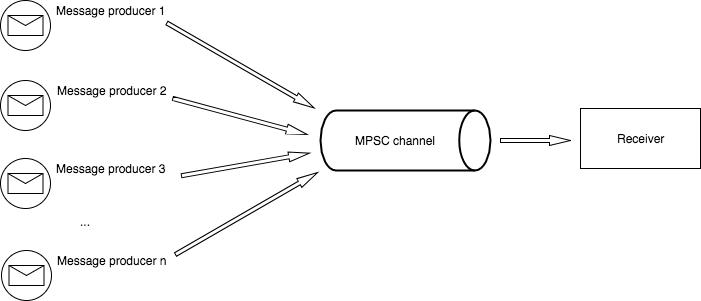
\includegraphics[width=0.8\textwidth]{images/mpsc.png}}
    \end{center}
    \caption{Canal de communication entre threads - \cite{ref37}}
    \label{rust_channel}
\end{figure}
\bigbreak
\begin{code}
    \begin{minted}[bgcolor=mygray,breaklines,breaksymbol=,linenos,frame=single,stepnumber=1,tabsize=2]{rust}
use std::thread;
use std::sync::mpsc;

fn main() {
    let (tx, rx) = mpsc::channel();

    let new_tx = mpsc::Sender::clone(&tx);
    thread::spawn(move || {
        let val = String::from("Hello from first thread");
        new_tx.send(val).unwrap();
    });

    thread::spawn(move || {
        let val = String::from("Hello from second thread");
        tx.send(val).unwrap();
    });

    for received in rx {
        println!("Message from threads: {}", received);
    }
}
    \end{minted}
    \caption{\textit{Message passing} avec deux producteurs et un consommateur en Rust}
    \label{rust_thread_message}
\end{code}
\bigbreak
Des primitives plus bas niveau (Mutex) ainsi que des traits sont disponibles pour manipuler 
plus finement les threads en Rust. Pour plus de détails, se référer au chapitre 16 du \textit{book} \cite{ref0}.
Un article illustrant l'utilisation des threads en Rust par la réalisation d'un programme simple 
de calcul de hash donne une bonne base pour construire son propre programme \cite{ref37}.

%%%%%%%%%%%%%%%%%%%%%%%%%%%%%%%%%%%%%%%%%%%%%%%%%%%%%%%%%%%%%%%%%%%%%%%%%%%%%%%%%%%%%%%%%%%%%%%%%%%
%%%%%%%%%%%%%%%%%%%%%%%%%%%%%%%%%%%%%%%%%%%%%%%%%%%%%%%%%%%%%%%%%%%%%%%%%%%%%%%%%%%%%%%%%%%%%%%%%%%
\subsubsection{\textit{Unsafe} Rust}
Le compilateur Rust est non seulement très verbeux lors d'erreurs mais également très restrictif. 
Cette contrainte est la garantie pour le programmeur d'obtenir un code sûr et fiable sur la gestion 
de la mémoire. Cependant, il arrive que du code doive transgresser les règles et bonnes pratiques
de Rust sur la mémoire. C'est notamment le cas pour du code bas niveau (manipulation du kernel par 
exemple). Pour ces cas de figure, Rust peut fonctionner en mode \textit{unsafe} ("non sûr"). Tout 
bloc de code qui nécessite d'être non sûr doit être précédé du mot-clé \mintinline{rust}{unsafe}. 
Il est alors de la responsabilité du programmeur de vérifier que le code n'est pas buggé ou dangereux.
Pour plus de détails, se référer au chapitre 19.1 du \textit{book} \cite{ref0}.

%%%%%%%%%%%%%%%%%%%%%%%%%%%%%%%%%%%%%%%%%%%%%%%%%%%%%%%%%%%%%%%%%%%%%%%%%%%%%%%%%%%%%%%%%%%%%%%%%%%
%%%%%%%%%%%%%%%%%%%%%%%%%%%%%%%%%%%%%%%%%%%%%%%%%%%%%%%%%%%%%%%%%%%%%%%%%%%%%%%%%%%%%%%%%%%%%%%%%%%
\subsection{Extended attributes}\label{extended_attributes}

%%%%%%%%%%%%%%%%%%%%%%%%%%%%%%%%%%%%%%%%%%%%%%%%%%%%%%%%%%%%%%%%%%%%%%%%%%%%%%%%%%%%%%%%%%%%%%%%%%%
%%%%%%%%%%%%%%%%%%%%%%%%%%%%%%%%%%%%%%%%%%%%%%%%%%%%%%%%%%%%%%%%%%%%%%%%%%%%%%%%%%%%%%%%%%%%%%%%%%%
\subsubsection{Fonctionnement des \acrshort{xattr}}
Les \textit{extended attributes} (\acrshort{xattr}), ou "attributs étendus" en français, sont un moyen d'attacher des 
méta-données aux fichiers et dossiers sous forme de paires \mintinline{text}{espace.nom:valeur}. 
L'espace de nom, ou \textit{namespace} en anglais, définit les différentes classes d'attributs. 
Dans le cadre de ce projet, l'accent est mis sur le système de fichiers (\acrshort{fs}) ext4 \cite{ref36}
sous Linux, il existe actuellement quatre espaces de noms 
ou classes : \mintinline{text}{user}, \mintinline{text}{trusted}, \mintinline{text}{security} et 
\mintinline{text}{system}. L'espace qui nous intéresse est \mintinline{text}{user}. C'est là que 
l'utilisateur ou l'application, pour autant qu'il ait les droits usuels UNIX sur les fichiers, peut 
manipuler les \acrshort{xattr}. Les trois autres espaces de noms sont utilisés entre autres pour 
les listes d'accès ACL (\mintinline{text}{system}), les modules de sécurité du kernel 
(\mintinline{text}{security}) ou par \mintinline{text}{root} (\mintinline{text}{trusted})
\cite{ref11} \cite{ref12}.
Le nom est une chaine de caractères et la valeur peut être une chaine de caractères ou des données binaires. 
Les \acrshort{xattr} sont stockés dans les fichiers. De nombreux \acrshort{fs} gèrent leur 
usage : ext2-3-4, XFS, Btrfs, UFS1-2, NTFS, HFS+, ZFS. Ces \acrshort{fs} sont utilisés par 
les quatre \acrshort{os} les plus répandus : Windows, macOS, Linux et FreeBSD. Windows utilise 
les \acrshort{xattr} notamment dans sa gestion des permissions Unix dans le shell Linux intégré 
à Windows 10 \cite{ref21}. macOS, comme vu à la section \ref{existant_macOS}, les utilise entre 
autres dans son système de gestion des tags. La commande \mintinline{text}{xattr} permet de les 
manipuler. Sous Linux, il en existe trois : \mintinline{text}{attr}, \mintinline{text}{getfattr} et 
\mintinline{text}{setfattr}. Sous Linux avec ext2-3-4, chaque attribut dispose d'un bloc de données 
(1024, 2048 ou 4096 bytes) \cite{ref12}.
Apple et freedesktop.org préconisent la notation DNS inversée pour 
nommer les attributs \cite{ref8}, \cite{ref24} car n'importe quel processus peut modifier les 
attributs dans l'espace utilisateur. En préfixant du nom du programme au nom de l'attribut, par 
exemple \mintinline{text}{user.myprogram.myattribute}, on diminue le risque qu'une autre 
application utilise le même nom d'attribut. Malheureusement, la plupart des outils \acrshort{cli} Linux 
pour manipuler les fichiers comme \mintinline{text}{cp}, \mintinline{text}{tar}, etc. ne prennent 
pas en compte les attributs avec leur syntaxe par défaut, il faut spécifier des arguments supplémentaires \cite{ref4}.

%%%%%%%%%%%%%%%%%%%%%%%%%%%%%%%%%%%%%%%%%%%%%%%%%%%%%%%%%%%%%%%%%%%%%%%%%%%%%%%%%%%%%%%%%%%%%%%%%%%
%%%%%%%%%%%%%%%%%%%%%%%%%%%%%%%%%%%%%%%%%%%%%%%%%%%%%%%%%%%%%%%%%%%%%%%%%%%%%%%%%%%%%%%%%%%%%%%%%%%
\subsubsection{Comportement lors des opérations d'accès courantes}
Pour vérifier la portabilité des \acrshort{xattr}, quelques tests ont été réalisés entre un 
SSD faisant office de disque système à Linux Mint 18.2 Sonya avec deux clés USB (de 8 et 64 Go) et un emplacement 
réseau monté en NFS. Le listing \ref{xattr_df} montre la sortie de la commande \mintinline{bash}{df}, qui 
renvoie l'utilisation des différents emplacements de stockage, dans l'ordre : le disque système, en 
ext4, la clé de 8 Go formatée une fois en FAT32, puis une autre fois en NTFS, la clé de 64 Go formatée 
en ext4 et finalement une machine virtuelle sous Debian 9 montée en NFS.
\bigbreak
\begin{code}
    \begin{minted}[bgcolor=mygray,breaklines,breaksymbol=,linenos,frame=single,stepnumber=1,tabsize=2]{text}
Sys. de fichiers        Type   Taille Utilisé Dispo Uti% Monté sur
/dev/sda2               ext4     451G    334G   96G  78% /
/dev/sdg1               vfat     7.7G    4.0K  7.7G   1% /media/pc/cle1
/dev/sdg1               fuseblk  7.7G     41M  7.7G   1% /media/pc/cle1
/dev/sdg1               ext4      59G     33G   23G  59% /media/pc/cle2
192.168.1.21:/home/user nfs4     916G    198G  673G  23% /mnt/debian
    \end{minted}
    \caption{Output de \mintinline{bash}{df -Th} : le disque système, les clés USB et le NFS}
    \label{xattr_df}
\end{code}
\bigbreak
La démarche est la suivante : un \acrshort{xattr} dans l'espace \mintinline{text}{user} avec 
comme nom \mintinline{text}{author} et comme valeur \mintinline{text}{steven} est ajouté au fichier 
\mintinline{text}{file.txt} avec \mintinline{bash}{attr}. Ce fichier est copié avec 
\mintinline{bash}{cp} en prenant garde à préserver l'attribut (option 
\mintinline{bash}{--preserve=xattr}). Une fois copié, on tente de lire le même attribut, toujours 
avec \mintinline{bash}{attr}. Les résultats sont visibles dans les listings \ref{xattr_copy_8_fat32}, 
\ref{xattr_copy_8_ntfs}, \ref{xattr_copy_64_ext4} et \ref{xattr_copy_nfs} :
\bigbreak
\begin{code}
    \inputminted[bgcolor=mygray,breaklines,breaksymbol=,linenos,frame=single,stepnumber=1,
        tabsize=2,firstline=45,lastline=49]{text}{text/test_attr.txt}
    \caption{Copie sur clé USB 8 Go, FAT32}
    \label{xattr_copy_8_fat32}
\end{code}
\bigbreak
\begin{code}
    \inputminted[bgcolor=mygray,breaklines,breaksymbol=,linenos,frame=single,stepnumber=1,
        tabsize=2,firstline=54,lastline=61]{text}{text/test_attr.txt}
    \caption{Copie sur clé USB 8 Go, NTFS}
    \label{xattr_copy_8_ntfs}
\end{code}
\bigbreak
\begin{code}
    \inputminted[bgcolor=mygray,breaklines,breaksymbol=,linenos,frame=single,stepnumber=1,
        tabsize=2,firstline=66,lastline=73]{text}{text/test_attr.txt}
    \caption{Copie sur clé USB 64 Go, ext4}
    \label{xattr_copy_64_ext4}
\end{code}
\bigbreak
\begin{code}
    \inputminted[bgcolor=mygray,breaklines,breaksymbol=,linenos,frame=single,stepnumber=1,
        tabsize=2,firstline=78,lastline=79]{text}{text/test_attr.txt}
    \caption{Copie sur l'emplacement réseau distant, NFS}
    \label{xattr_copy_nfs}
\end{code}
\bigbreak
On constate que l'opération est infructueuse sur la clé en FAT32 et sur l'emplacement réseau monté 
en NFS alors qu'elle réussit sur les clés USB en NTFS et ext4. 
\\
Deux autres petites expériences ont 
été menées avec la commande \mintinline{bash}{mv} et la copie/déplacement de fichiers avec 
l'explorateur de fichiers Nemo de Linux Mint. Ces deux opérations conservent par défaut les \acrshort{xattr}.

%%%%%%%%%%%%%%%%%%%%%%%%%%%%%%%%%%%%%%%%%%%%%%%%%%%%%%%%%%%%%%%%%%%%%%%%%%%%%%%%%%%%%%%%%%%%%%%%%%%
%%%%%%%%%%%%%%%%%%%%%%%%%%%%%%%%%%%%%%%%%%%%%%%%%%%%%%%%%%%%%%%%%%%%%%%%%%%%%%%%%%%%%%%%%%%%%%%%%%%
\subsection{\mintinline{c}{inotify}}\label{inotify_techno}
Sous Linux, un outil (inclu au noyau) dédié à la surveillance du \acrshort{fs} existe, \mintinline{c}{inotify} 
\cite{ref29}. Comme son nom l'indique, \mintinline{c}{inotify} donne la possibilité à une application d'être 
notifiée sur des événements au niveau du système de fichiers. Une interface de programmation (\acrshort{api}) 
en C existe et offre les appels systèmes (\acrshort{syscall}) suivants :
\begin{enumerate}
    \item \mintinline{c}{int inotify_init(void)} : initialise une instance \mintinline{c}{inotify} et retourne un 
        descripteur de fichier.
    \item \mintinline{c}{int inotify_add_watch(int fd, const char *pathname, uint32_t mask)} : 
        cette fonction attend le descripteur de fichier renvoyé par \mintinline{c}{inotify_init}, 
        un chemin de fichier ou répertoire à surveiller et un masque binaire constitué des 
        événements à surveiller (voir plus loin). Il retourne un nouveau descripteur de fichier 
        qui pourra être lu avec le \acrshort{syscall} \mintinline{c}{read()}.
    \item \mintinline{c}{int inotify_rm_watch(int fd, int wd)} : appel inverse du précédent, 
        supprime la surveillance du descripteur de fichier \mintinline{c}{wd} de l'instance \mintinline{c}{inotify} 
        retournée par \mintinline{c}{fd}.
\end{enumerate}
\mintinline{c}{inotify} s'utilise comme suit : il faut initialiser l'instance, ajouter les fichiers et répertoires 
pour la surveillance avec le masque des événements voulus et, généralement, dans une boucle, 
appeler le \acrshort{syscall} \mintinline{c}{read()} avec comme argument le descripteur de fichier 
renvoyé par \mintinline{c}{inotify_init()}. Chaque appel abouti à \mintinline{c}{read()} retourne 
la structure disponible au listing \ref{inotify_struct_event} :
\bigbreak
\begin{code}
    \begin{minted}[bgcolor=mygray,breaklines,breaksymbol=,linenos,frame=single,stepnumber=1,tabsize=2]{c}
struct inotify_event {
    int      wd;       /* Descripteur de surveillance */
    uint32_t mask;     /* Masque d'événements */
    uint32_t cookie;   /* Cookie unique d'association des
                          événements (pour rename(2)) */
    uint32_t len;      /* Taille du champ name */
    char     name[];   /* Nom optionnel terminé par un nul */
};
    \end{minted}
    \caption{Structure \mintinline{c}{inotify_event} - \cite{ref29}}
    \label{inotify_struct_event}
\end{code}
\bigbreak
Le champ \mintinline{c}{mask} peut prendre les valeurs suivantes (multiples valeurs autorisées, 
séparées par des "ou" logiques -> "|") :
\begin{itemize}
    \item IN\_ACCESS : accès au fichier.
    \item IN\_ATTRIB : changement sur les attributs du fichier.
    \item IN\_CLOSE\_WRITE : fichier ouvert en écriture fermé.
    \item IN\_CLOSE\_NOWRITE : fichier ouvert en écriture fermé.
    \item IN\_CREATE : création de fichier/répertoire.
    \item IN\_DELETE : suppression d'un fichier/répertoire.
    \item IN\_DELETE\_SELF : suppression du répertoire surveillé lui-même.
    \item IN\_MODIFY : modification d'un fichier/répertoire.
    \item IN\_MOVE\_SELF : suppression d'un fichier/répertoire.
    \item IN\_MOVE\_FROM : déplacement/renommage du répertoire (ancien nom).
    \item IN\_MOVE\_TO : déplacement/renommage du répertoire (nouveau nom).
    \item IN\_OPEN : ouverture d'un fichier.
    \item IN\_ALL\_EVENTS : macro combinant tous les événements précédents.
\end{itemize}
Le champ \mintinline{c}{cookie} de la structure \mintinline{c}{inotify_event} prend tout son sens 
lors des événements IN\_MOVE : un numéro unique est généré pour faire le lien entre ces deux 
sous-événements, qui ne sont en réalité qu'un seul. \mintinline{c}{inotify} offre donc une très bonne base pour 
la surveillance du \acrshort{fs}. Il possède cependant quelques limitations :
\begin{itemize}
    \item Pas de surveillance récursive d'un répertoire : si une arborescence complète doit être 
        surveillée, il faut pour chaque sous-répertoire ajouter une surveillance dédiée.
    \item Les chemins de fichiers peuvent changer entre l'émission d'un événement et son traitement.
    \item \mintinline{c}{inotify} ne permet que la surveillance de répertoires en espace utilisateur par défaut.
    \item Il n'y pas de moyen de discriminer quel processus ou utilisateur a généré un événement.
\end{itemize}
Il existe plusieurs outils système qui utilisent \mintinline{c}{inotify} \cite{ref30} :
\begin{itemize}
    \item \mintinline{bash}{incron} : équivalent de \mintinline{bash}{cron}, mais l'exécution 
        des tâches se fait non pas selon un horaire donné, mais selon un événement donné sur un fichier.
    \item \mintinline{bash}{lsyncd} : outil de synchronisation, basé sur \mintinline{bash}{rsync}. 
        La synchronisation est effectuée à chaque changement dans le répertoire surveillé vers une 
        liste d'emplacements distants configurés à l'avance.
    \item \mintinline{bash}{iwatch} : déclenchement d'une commande selon un événement \mintinline{bash}{inotify}.
    \item \mintinline{bash}{inotify-tools} : deux commandes permettant d'utiliser \mintinline{bash}{inotify} 
        directement dans le terminal :
        \begin{itemize}
            \item \mintinline{bash}{inotifywait} : exécute une attente sur un événement, avant de 
                continuer le fil d'exécution.
            \item \mintinline{bash}{inotifywatch} : retourne une liste d'événements des répertoires surveillés.
        \end{itemize}
\end{itemize}
Pour plus d'informations, la page de \mintinline{text}{man} sur \mintinline{c}{inotify} existe \cite{ref29} et 
un très bon article en deux parties sur les ajouts de \mintinline{c}{inotify} par rapport à \mintinline{c}{dnotify} 
(son prédécesseur) \cite{ref31} et sur ses limitations par Michael Kerrisk \cite{ref32}.
\\
Pour conclure, il existe également une \acrshort{api} plus récente pour recevoir les notifications du 
\acrshort{fs}, \mintinline{text}{fanotify} \cite{ref38}. Elle gomme quelques défauts d'\mintinline{c}{inotify}
(notamment l'accès aux périphériques montés, tels que les clé USB), mais comporte un défaut de taille 
pour ce projet : il n'y pas le support les événements de création, suppression et déplacement de fichiers 
et répertoires. \mintinline{c}{fanotify} ne peut donc pas être utilisé pour ce projet.

%%%%%%%%%%%%%%%%%%%%%%%%%%%%%%%%%%%%%%%%%%%%%%%%%%%%%%%%%%%%%%%%%%%%%%%%%%%%%%%%%%%%%%%%%%%%%%%%%%%
%%%%%%%%%%%%%%%%%%%%%%%%%%%%%%%%%%%%%%%%%%%%%%%%%%%%%%%%%%%%%%%%%%%%%%%%%%%%%%%%%%%%%%%%%%%%%%%%%%%
\subsection{\textit{Sockets}}\label{sockets_doc}
Les \textit{sockets} (littéralement "prise" en français) sont un moyen de communication entre 
différents processus, qu'ils soient sur la même machine ou en réseau. Il existe plusieurs types 
de \textit{sockets}, les deux plus connues sont les sockets "locales" (type \mintinline{c}{AF_UNIX} ou 
\mintinline{c}{AF_LOCAL}), uniquement possibles sur la même machine car reliées par un fichier spécial 
sur le \acrshort{fs} de la machine et les sockets IP (type \mintinline{c}{AF_INET} ou 
\mintinline{c}{AF_INET6}) qui sont reliées par des paires d'adresses IP et ports.
Lors d'une communication socket entre deux processus, un des processus endosse le rôle de serveur 
l'autre de client. Le serveur doit, dans l'ordre, exécuter les \acrshort{syscall} suivants : 
\begin{enumerate}
    \item Créer la socket avec \mintinline{c}{socket()}.
    \item Associer la socket à une adresse d'écoute avec \mintinline{c}{bind()}.
    \item Écouter l'arrivée d'une connexion avec \mintinline{c}{listen()}.
    \item Accepter une connexion entrante avec \mintinline{c}{accept()}.
    \item Recevoir les messages avec \mintinline{c}{read()}.
    \item Émettre les messages avec \mintinline{c}{write()}.
    \item Fermer la connexion avec \mintinline{c}{close()}.
\end{enumerate}
Le client, de son côté, doit exécuter les \acrshort{syscall} suivants :
\begin{enumerate}
    \item Créer la socket avec \mintinline{c}{socket()}.
    \item Se connecter à un serveur en écoute avec \mintinline{c}{connect()}.
    \item Recevoir les messages avec \mintinline{c}{read()}.
    \item Émettre les messages avec \mintinline{c}{write()}.
    \item Fermer la connexion avec \mintinline{c}{close()}.
\end{enumerate}
La figure \ref{sockets_procedure} résume la procédure d'initialisation et d'utilisation des sockets.
\begin{figure}
    \begin{center}
        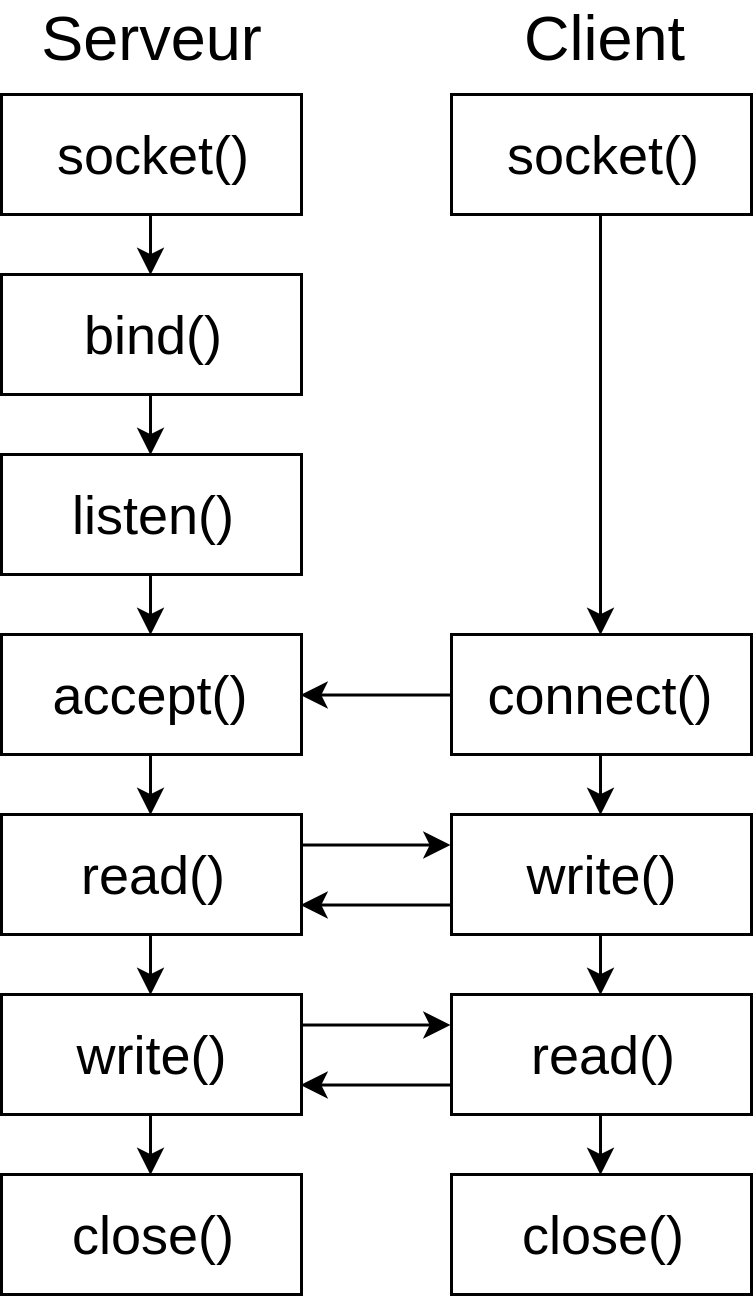
\includegraphics[width=0.4\textwidth]{images/sockets.png}
    \end{center}
    \caption{Procédure d'initialisation et d'utilisation des sockets}
    \label{sockets_procedure}
\end{figure}
Lors de l'établissement de la connexion, un canal est établi entre les deux processus, tout ce que 
le serveur écrit est reçu par le client et inversement. Pour plus d'informations, la page de man 
des sockets est disponible \cite{ref39}.

\newpage

\section{Réalisation} %-----------------------------------------------------------------------------------------------
%%%%%%%%%%%%%%%%%%%%%%%%%%%%%%%%%%%%%%%%%%%%%%%%%%%%%%%%%%%%%%%%%%%%%%%%%%%%%%%%%%%%%%%%%%%%%%%%%%%
%%%%%%%%%%%%%%%%%%%%%%%%%%%%%%%%%%%%%%%%%%%%%%%%%%%%%%%%%%%%%%%%%%%%%%%%%%%%%%%%%%%%%%%%%%%%%%%%%%%
\subsection{Tag Manager}\label{tag_manager}

%%%%%%%%%%%%%%%%%%%%%%%%%%%%%%%%%%%%%%%%%%%%%%%%%%%%%%%%%%%%%%%%%%%%%%%%%%%%%%%%%%%%%%%%%%%%%%%%%%%
%%%%%%%%%%%%%%%%%%%%%%%%%%%%%%%%%%%%%%%%%%%%%%%%%%%%%%%%%%%%%%%%%%%%%%%%%%%%%%%%%%%%%%%%%%%%%%%%%%%
\subsubsection{Description du programme et du code}\label{tag_manager_description}
La première réalisation de ce projet est un outil en ligne de commande (\acrshort{cli}), écrit en Rust, permettant 
de facilement lister, ajouter et supprimer des tags à des fichiers et répertoires (avec une option 
récursive pour ces derniers) et d'exécuter des requêtes vers le serveur (Tag Engine, sous-section 
\ref{tag_engine_realisation}) pour lister 
les tags existants, renommer un tag et demander la liste des fichiers correspondant à des tags 
donnés. Cet outil dépend de deux \textit{crates} disponibles sur \href{https://crates.io}{crates.io} 
: clap \cite{ref22} et xattr \cite{ref23}. Les tags sont stockés dans un \textit{extended attribute} 
(\acrshort{xattr}) nommé \mintinline{text}{user.tags} et sont séparés entre eux par des virgules.

\subparagraph{clap}
(Command Line Argument Parser for Rust) est une 
librairie pour \textit{parse} les arguments d'un programme \acrshort{cli}. Elle analyse 
et valide les arguments fournis par l'utilisateur. Elle dispose de plusieurs syntaxes pour 
définir les arguments des commandes et options attendues par notre programme. 
Sur le dépôt github de clap, dans le 
dossier \textit{examples}, plusieurs exemples d'utilisation sont fournis. Pour illustrer son 
utilisation, le listing \ref{tag_manager_clap} reprend l'exemple \mintinline{text}{01a_quick_example.rs} 
avec la plupart des commentaires tronqués et des adaptations de mise en page. Des lignes 2 à 13, 
les arguments attendus et les informations sur l'application sont définis avec entre autres la 
version du programme, le nom de l'auteur, etc. Dans cet exemple, les arguments sont définis à 
partir d'une chaîne de caractères respectant un format bien spécifique. clap génère automatiquement 
une aide au programme à partir des arguments définis s'il est lancé sans aucun des arguments obligatoires.
À partir de la ligne 15, les arguments reçus sont utilisés. La méthode \mintinline{rust}{value_of()} 
retourne la valeur d'un argument présent à l'exécution. Il est donc aisé d'utiliser les arguments 
donnés en tant que variables du programme. clap donne également la possibilité de regrouper les 
arguments. Un seul argument d'un groupe peut être présent à l'exécution, ce qui évite de nombreuses 
conditions de détection et d'exclusion des arguments.

\subparagraph{xattr}
est une interface de programmation (\acrshort{api}) 
en Rust pour récupérer, lister, ajouter/modifier et supprimer des \acrshort{xattr} accrochés à des 
fichiers avec Rust. C'est essentiellement un \textit{wrapper} des appels système (\acrshort{syscall}) en C fournis par Linux 
et d'autres systèmes d'exploitation (\acrshort{os}) pour manipuler les \acrshort{xattr}. À noter que les fonctions offertes ne 
suivent pas les liens symboliques (il est fait de même pour Tag Manager lui-même). Quatre fonctions 
sont disponibles : \mintinline{rust}{get()}, \mintinline{rust}{list()}, \mintinline{rust}{set()} 
et \mintinline{rust}{remove()}. Toutes attendent le nom du fichier et selon les cas le nom du 
\acrshort{xattr} ainsi que sa valeur.
\bigbreak
\begin{code}
    \begin{minted}[bgcolor=mygray,breaklines,breaksymbol=,linenos,frame=single,stepnumber=1,tabsize=2]{rust}
fn main() {
    let matches = App::new("MyApp")
        .version("1.0")
        .author("Kevin K. <kbknapp@gmail.com>")
        .about("Does awesome things")
        .args_from_usage(
            "-c, --config=[FILE] 'Sets a custom config file'
            <output> 'Sets an optional output file'
            -d... 'Turn debugging information on'")
        .subcommand(SubCommand::with_name("test")
            .about("does testing things")
            .arg_from_usage("-l, --list 'lists test values'"))
        .get_matches();

    if let Some(o) = matches.value_of("output") {
        println!("Value for output: {}", o);
    }
    if let Some(c) = matches.value_of("config") {
        println!("Value for config: {}", c);
    }

    match matches.occurrences_of("d") {
        0 => println!("Debug mode is off"),
        1 => println!("Debug mode is kind of on"),
        2 => println!("Debug mode is on"),
        3 | _ => println!("Don't be crazy"),
    }

    if let Some(matches) = matches.subcommand_matches("test") {
        if matches.is_present("list") {
            println!("Printing testing lists...");
        } else {
            println!("Not printing testing lists...");
        }
    }
}
    \end{minted}
    \caption{Exemple d'utilisation de clap (commentaires tronqués) - \cite{ref42}}
    \label{tag_manager_clap}
\end{code}
\bigbreak
Tag Manager est constitué de deux fichiers. Le premier, \mintinline{rust}{main.rs} contient les 
définitions et détections des arguments fournis par l'utilisateur avec clap (voir listing 
\ref{tag_manager_main_args}), les appels aux fonctions 
manipulant les tags des fichiers et la partie socket de connexion, requêtes et attente 
de réponse du serveur (Tag Engine, sous-section \ref{tag_engine_realisation}). Le deuxième fichier, 
\mintinline{rust}{lib.rs}, contient l'\acrshort{api} publique pour récupérer, attribuer, renommer 
et supprimer les tags pour un fichier donné et un module de test de ces fonctions. À noter que 
dans les \textit{output} du programme, il n'y a pas de distinction entre fichiers et répertoires.
À titre d'exemple, 
le listing \ref{tag_manager_del_tags} montre le code de la fonction \mintinline{rust}{del_tags()} 
qui supprime les tags donnés d'un fichier. Elle préserve les tags existants qui ne doivent pas être 
supprimés et supprime totalement le \acrshort{xattr} en cas de tableau de tags vide. L'usage 
des \mintinline{rust}{enum} \mintinline{rust}{Option} et \mintinline{rust}{Result} en association 
avec des \textit{pattern matching} sont utilisées dès que possible.
\bigbreak
\begin{code}
    \inputminted[bgcolor=mygray,breaklines,breaksymbol=,linenos,frame=single,stepnumber=1,
        tabsize=2,firstline=43,lastline=62]{rust}{../tag_manager/src/main.rs}
    \caption{Déclaration des arguments dans \mintinline{rust}{main.rs}}
    \label{tag_manager_main_args}
\end{code}
\bigbreak
\bigbreak
\begin{code}
    \inputminted[bgcolor=mygray,breaklines,breaksymbol=,linenos,frame=single,stepnumber=1,
        tabsize=2,firstline=55,lastline=82]{rust}{../tag_manager/src/lib.rs}
    \caption{Code de la fonction \mintinline{rust}{del_tags()} dans \mintinline{rust}{lib.rs}}
    \label{tag_manager_del_tags}
\end{code}
\bigbreak
La communication socket est réalisée grâce la librairie standard \mintinline{rust}{UnixStream}, 
équivalent aux sockets \mintinline{c}{AF_UNIX} en C (voir sous-section \ref{sockets_doc}). Le 
fichier adresse des sockets est par défaut écrit dans \mintinline{text}{/tmp/tag_engine}. Le format 
des requêtes respecte le petit protocole décrit dans la table \ref{tag_manager_sockets_protocol}. 
Le début de la requête est formé du code à trois caractères.
La requête listant les fichiers selon une expression logique des tags accepte les opérateurs 
\mintinline{text}{AND} et \mintinline{text}{OR}, avec la précédence logique du premier sur le 
second (voir sous-section \ref{tag_engine_realisation} pour plus de détails). Les opérateurs et 
opérandes (les tags) doivent être séparés par un espace.
\begin{center}
    \begin{tabular}{|p{7cm}|c|p{6cm}|} \hline
        \textbf{Requête} & \textbf{Code} & \textbf{Exemple} \\ \hline
        Fichiers et répertoires correspondants à une expression logique de tags & \mintinline{text}{0x0} & 
            \mintinline{text}{0x0 tag1 OR tag2 AND tag3} \\ \hline
        Liste des tags existants & \mintinline{text}{0x1} & \mintinline{text}{0x1} \\ \hline
        Renommage d'un tag & \mintinline{text}{0x2} & \mintinline{text}{0x2 old_name new_name} \\ \hline
    \end{tabular}
    \captionof{table}{Format du protocole des requêtes au serveur Tag Engine}
    \label{tag_manager_sockets_protocol}
\end{center}
La figure \ref{tag_manager_schema} résume le fonctionnement du programme : 
\begin{enumerate}
    \item Analyse des arguments.
    \item Exécution des commandes (soit sur les fichiers, soit requête vers le serveur).
    \item Impression des résultats.
\end{enumerate}
\begin{figure}
    \begin{center}
        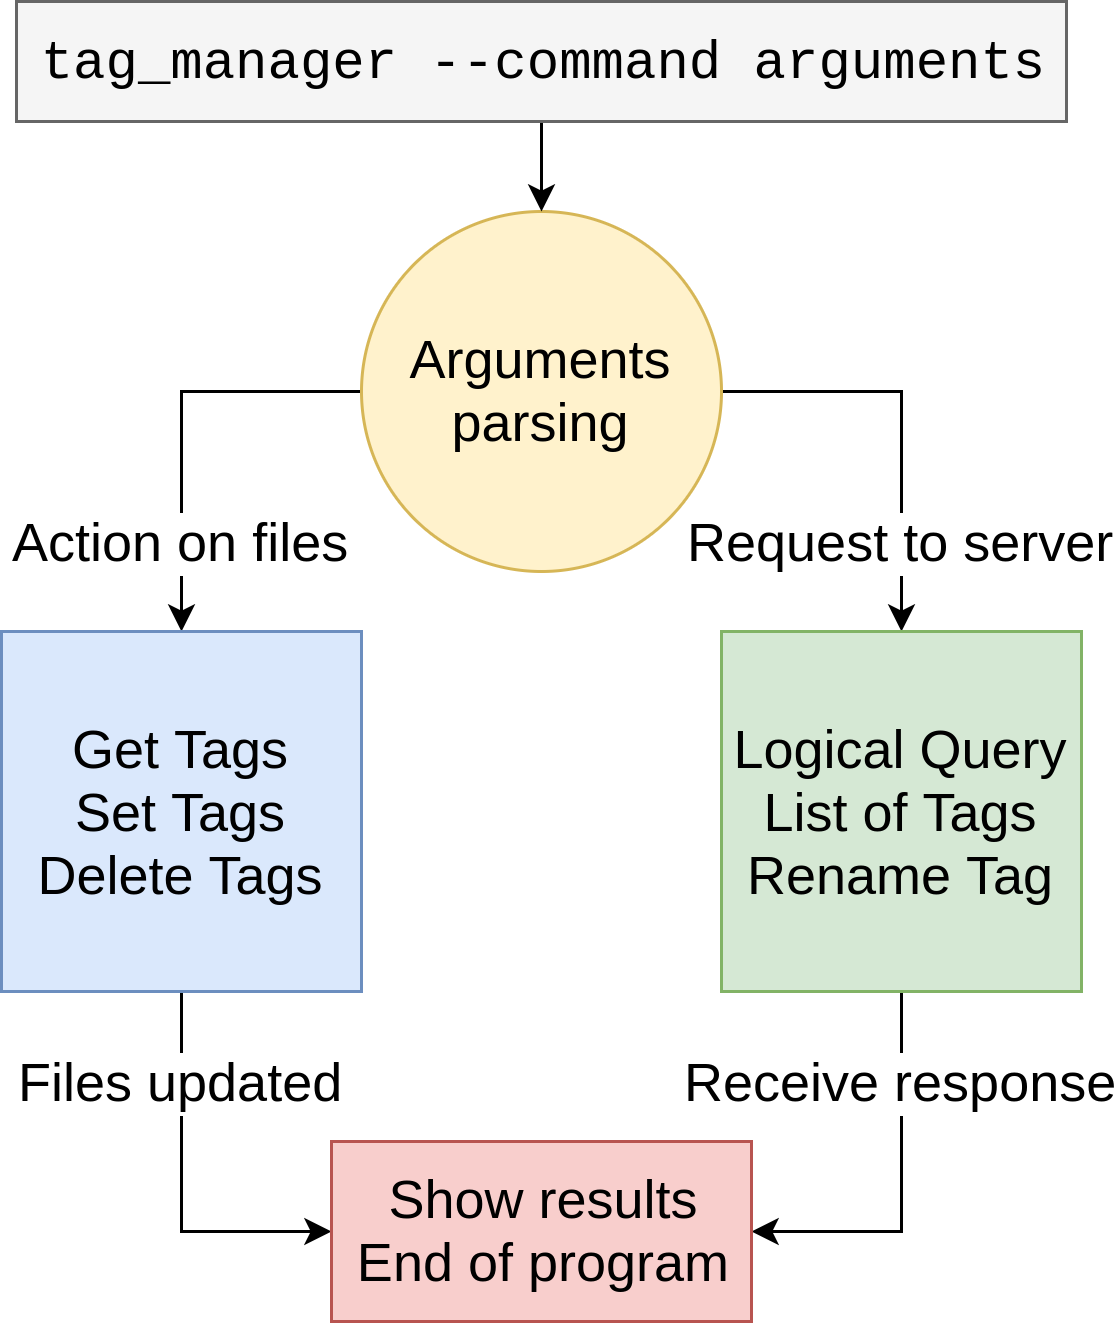
\includegraphics[width=0.6\textwidth]{images/tag_manager.png}
    \end{center}
    \caption{Schéma de fonctionnement de Tag Manager}
    \label{tag_manager_schema}
\end{figure}

%%%%%%%%%%%%%%%%%%%%%%%%%%%%%%%%%%%%%%%%%%%%%%%%%%%%%%%%%%%%%%%%%%%%%%%%%%%%%%%%%%%%%%%%%%%%%%%%%%%
%%%%%%%%%%%%%%%%%%%%%%%%%%%%%%%%%%%%%%%%%%%%%%%%%%%%%%%%%%%%%%%%%%%%%%%%%%%%%%%%%%%%%%%%%%%%%%%%%%%
\subsubsection{Utilisation du programme et exemples}\label{tag_manager_utilisation}
L'utilisation des différents arguments du programme est résumée dans la table \ref{tag_manager_usage}. 
Les arguments sont divisés en deux groupes, le premier pour manipuler directement les fichiers et 
leurs tags, le deuxième pour exécuter des requêtes vers le serveur Tag Engine. Pour le premier groupe, 
l'argument \mintinline{text}{-f} ou \mintinline{text}{--files} est obligatoire. Pour les opérations 
du deuxième groupe, il faut évidemment que le serveur Tag Engine soit lancé.
\begin{center}
    \begin{tabular}{|p{3.7cm}|p{2.3cm}|p{8.5cm}|} \hline
        \textbf{Opération} & \textbf{Arguments} & \textbf{Exemple} \\ \hline
        Afficher l'aide & \mintinline{text}{-h} & \mintinline{text}{tag_manager -h} \\ \hline
        Afficher les tags d'un ou plusieurs fichiers & 
            \mintinline{text}{-f} ou \mintinline{text}{--files} & 
            \mintinline{text}{tag_manager -f file1 file2} \\ \hline
        Afficher les tags d'un dossier récursivement & 
            \mintinline{text}{-r} ou \mintinline{text}{--recursive} & 
            \mintinline{text}{tag_manager -f myfolder -r} \\ \hline
        Attribuer des tags à un ou plusieurs fichiers & 
            \mintinline{text}{-s} ou \mintinline{text}{--set} & 
            \mintinline{text}{tag_manager -f file1 file2 -s bob fred} \\ \hline
        Supprimer des tags à un ou plusieurs fichiers & 
            \mintinline{text}{-d} ou \mintinline{text}{--del} & 
            \mintinline{text}{tag_manager -f file1 file2 -d bob fred} \\ \hline
        Lister les fichiers correspondants à une requête de tags & 
            \mintinline{text}{-q} ou \mintinline{text}{--query} & 
            \mintinline{text}{tag_manager -q bob AND fred} \\ \hline
        Lister les tags existants & 
            \mintinline{text}{-l} ou \mintinline{text}{--list} & 
            \mintinline{text}{tag_manager -l} \\ \hline
        Renommer un tag & 
            \mintinline{text}{-R} ou \mintinline{text}{--rename} & 
            \mintinline{text}{tag_manager -R old_name new_name} \\ \hline
    \end{tabular}
    \captionof{table}{Utilisation et arguments attendus par Tag Manager}
    \label{tag_manager_usage}
\end{center}
Le listing \ref{tag_manager_ex} illustre les usages et retours de Tag Manager. Tout d'abord, Tag Manager est utilisé pour 
lister récursivement les tags des fichiers et sous-répertoires donnés, attribuer les tags \mintinline{text}{in_a} 
et \mintinline{text}{myfiles} à différents fichiers et répertoires, lister les tags existants et faire 
une requête sur les deux tags. L'arborescence utilisée pour l'exemple est constituée des quatre fichiers 
et deux répertoires suivants :
\dirtree{%
.1 a.
.2 a1.
.2 a2.
.2 b.
.3 b1.
.3 b2.
}
\bigbreak
\begin{code}
    \inputminted[bgcolor=mygray,breaklines,breaksymbol=,linenos,frame=single,stepnumber=1,
        tabsize=2]{bash}{text/tag_manager_ex.txt}
    \caption{Exemples d'utilisation de Tag Manager}
    \label{tag_manager_ex}
\end{code}
\bigbreak

%%%%%%%%%%%%%%%%%%%%%%%%%%%%%%%%%%%%%%%%%%%%%%%%%%%%%%%%%%%%%%%%%%%%%%%%%%%%%%%%%%%%%%%%%%%%%%%%%%%
%%%%%%%%%%%%%%%%%%%%%%%%%%%%%%%%%%%%%%%%%%%%%%%%%%%%%%%%%%%%%%%%%%%%%%%%%%%%%%%%%%%%%%%%%%%%%%%%%%%
\subsection{Tag Engine}\label{tag_engine_realisation}

%%%%%%%%%%%%%%%%%%%%%%%%%%%%%%%%%%%%%%%%%%%%%%%%%%%%%%%%%%%%%%%%%%%%%%%%%%%%%%%%%%%%%%%%%%%%%%%%%%%
%%%%%%%%%%%%%%%%%%%%%%%%%%%%%%%%%%%%%%%%%%%%%%%%%%%%%%%%%%%%%%%%%%%%%%%%%%%%%%%%%%%%%%%%%%%%%%%%%%%
\subsubsection{Description du programme et du code}
La deuxième réalisation pratique de ce projet est un programme indexant et surveillant une arborescence de 
répertoires, fichiers et tags associés. Ce programme fait également office de serveur pour les 
requêtes émises depuis Tag Manager. Il est divisé en plusieurs fichiers et modules :
\begin{itemize}
    \item \mintinline{rust}{graph.rs} : module relatif à la construction et 
        maintenance du graphe des tags, fichiers et répertoires (voir paragraphe \textbf{petgraph}).
    \item \mintinline{rust}{lib.rs} : regroupe les autres modules et contient la fonction 
        \mintinline{rust}{dispatcher()}, appelée lors d'un événement sur l'arborescence surveillée 
        (voir paragraphe \textbf{notify}).
    \item \mintinline{rust}{main.rs} : point d'entrée du programme, initialise les variables 
        partagées, le thread socket serveur et écoute indéfiniment sur les événements survenus 
        sur l'arborescence surveillée (voir paragraphe \textbf{Mutex et références multiples}).
    \item \mintinline{rust}{parse.rs} : module de conversion d'une expression infixe vers postfixe 
        (voir paragraphe \textbf{Analyse d'une expression logique}).
    \item \mintinline{rust}{server.rs} : module construisant le serveur socket et répondant 
        aux différentes requêtes émises depuis Tag Manager (voir paragraphe \textbf{Serveur sockets}).
\end{itemize}
Ce programme dépend de quatre \textit{crates} externes. Le premier est 
tag\_manager (la librairie des fonctions manipulant les \acrshort{xattr}, voir sous-section \ref{tag_manager}), 
réalisé au cours de ce projet. Les trois autres sont disponibles sur \href{https://crates.io}{crates.io}, 
il s'agit de walkdir \cite{ref43}, petgraph \cite{ref44} et notify \cite{ref45}.

\subparagraph{walkdir}
est une librairie pour parcourir efficacement et de manière récursive une arborescence de fichiers.
Elle offre différentes structures, dont \mintinline{rust}{WalkDir} et \mintinline{rust}{DirEntry}. 
\mintinline{rust}{WalkDir} attend un chemin de répertoire et retourne un itérateur listant 
chaque sous-répertoire et fichier contenu dans le répertoire de départ. Chaque entrée de cet 
itérateur est représenté par la structure \mintinline{rust}{DirEntry}, qui détient des méthodes 
pour obtenir des informations sur l'entrée (le chemin complet, les méta-données, si c'est un 
répertoire ou un fichier, son nom, etc.). Le listing \ref{walkdir_demo} illustre un exemple de 
parcours d'un répertoire et de l'affichage des informations pour chaque entrée rencontrée. 
walkdir est utilisé pour réaliser le premier balayage de l'arborescence 
fournie et constituer le graphe (voir listing \ref{tag_engine_graph_make_graph}).
\bigbreak
\begin{code}
    \begin{minted}[bgcolor=mygray,breaklines,breaksymbol=,linenos,frame=single,stepnumber=1,tabsize=2]{rust}
use walkdir::WalkDir;

fn main() {
    for entry in WalkDir::new("/home") {
        let entry = entry.unwrap();
        println!("{}", entry.path().display());
    }
}
    \end{minted}
    \caption{Parcours d'un répertoire avec walkdir}
    \label{walkdir_demo}
\end{code}
% \bigbreak

\subparagraph{petgraph}\label{tag_engine_petgraph}
est une librairie de représentation de graphes. Elle fournit différentes structures de données pour 
représenter un graphe et des modules de manipulation et parcours de graphes. Les structures de 
données sont au nombre de trois :
\begin{enumerate}
    \item \mintinline{rust}{Graph<N, E, Ty = Directed, Ix = DefaultIx>} : représente un graphe et 
        ses données sous forme de deux listes d'adjacences (deux \mintinline{rust}{Vec}, un pour les 
        noeuds et l'autre pour les arcs ou arêtes). Les noeuds sont de type générique \mintinline{rust}{N}, 
        les arcs ou arêtes de type générique \mintinline{rust}{E}, le graphe est par défaut orienté (type 
        \mintinline{rust}{Directed}) et le type pour l'index (l'identifiant numérique d'un noeud et 
        d'un arc ou arête dans les vecteurs respectifs, déterminant la taille maximale du graphe) 
        est par défaut \mintinline{rust}{u32} (ce qui autorise plus de quatre milliards de noeuds, 
        4'294'967'296 précisément).
    \item \mintinline{rust}{StableGraph<N, E, Ty = Directed, Ix = DefaultIx>} : semblable à 
        \mintinline{rust}{Graph}, avec une différence notable, elle garde les identifiants des noeuds et 
        arcs ou arêtes supprimés. Cette structure comporte également moins de méthodes.
    \item \mintinline{rust}{GraphMap<N, E, Ty>} : représente un graphe et ses données sous forme 
        d'une table associative, dont les clés sont les noeuds de type générique \mintinline{rust}{N}, 
        avec l'obligation pour ce type d'être conforme pour l'utilisation en tant que clé. Permet 
        de tester l'existence d'un noeud en temps constant avec la contrepartie de ne pas pouvoir 
        stocker plus qu'un noeud avec une même donnée.
\end{enumerate}
Avant de continuer les explications sur l'utilisation de petgraph, faisons un bref rappel de l'architecture 
choisie pour représenter l'arborescence des fichiers et tags à surveiller. Un noeud du graphe peut 
être soit un fichier, soit un répertoire, soit un tag. Le lien entre un répertoire et un sous-répertoire 
ou un fichier est symbolisé par un arc partant du répertoire en question. Le lien entre un tag et 
un répertoire ou un fichier est également un arc partant du tag en question. Un arc n'a pas de 
données à sauvegarder, il n'a donc pas de type effectif. Pour accélérer l'accès à un tag dans le 
graphe à partir de son nom, une \textit{hashmap} associant le nom du tag à son identifiant dans le graphe 
est maintenue.
\bigbreak
La structure \mintinline{rust}{StableGraph} a été choisie en raison de sa rétention des identifiants lors 
des suppressions de noeuds et d'arcs. En effet, lors des opérations de suppression de tags ou de 
fichiers, pour maintenir cohérente la \textit{hashmap} des tags associés aux identifiants du graphe, il 
ne faut pas que cesdits identifiants changent. Dans le cas contraire, cette \textit{hashmap} ne 
serait pas utilisable. Le listing \ref{tag_engine_graph_structs} montre les structures de données 
utilisées pour notre graphe. Un noeud du graphe est représenté par la structure \mintinline{rust}{Node}, 
contenant le nom du noeud et son genre (tag, fichier ou répertoire). Un arc est simplement défini 
par un type vide, nommé \mintinline{rust}{Nil}. petgraph offre de nombreuses méthodes pour 
\mintinline{rust}{StableGraph} : accès, ajout et suppression de noeuds et d'arcs, un itérateur sur 
les voisins d'un noeud (avec indication du sens), recherche d'arcs entre deux noeuds, etc. La 
fonction \mintinline{rust}{make_graph()} listée au listing \ref{tag_engine_graph_make_graph} est 
la fonction première de notre module, elle crée le graphe et la \textit{hashmap} avec walkdir à partir du
chemin du répertoire racine. Elle retourne le graphe contenant les fichiers, répertoires et tags 
trouvés, la \textit{hashmap} remplie et l'identifiant du noeud racine, point de départ pour les mises à 
jour suivantes du graphe (sur les fichiers et répertoires). La fonction \mintinline{rust}{make_subgraph()}, 
appelée dans la boucle s'assure d'ajouter correctement les noeuds en fonction du chemin, pour éviter 
de créer deux fois le même noeud ou pour qu'un noeud enfant ne soit créé avant son parent 
(il n'y a pas de garantie de parcourir l'arborescence des fichiers dans un ordre parent-enfants).
\bigbreak
\begin{code}
    \inputminted[bgcolor=mygray,breaklines,breaksymbol=,linenos,frame=single,stepnumber=1,
        tabsize=2,firstline=16,lastline=32]{rust}{../tag_engine/src/graph.rs}
    \caption{Structures pour les noeuds et les arcs du graphe dans \mintinline{rust}{src/graph.rs}}
    \label{tag_engine_graph_structs}
\end{code}
\bigbreak
\bigbreak
\begin{code}
    \inputminted[bgcolor=mygray,breaklines,breaksymbol=,linenos,frame=single,stepnumber=1,
        tabsize=2,firstline=83,lastline=108]{rust}{../tag_engine/src/graph.rs}
    \caption{Fonction \mintinline{rust}{make_graph()} dans \mintinline{rust}{src/graph.rs}}
    \label{tag_engine_graph_make_graph}
\end{code}
\bigbreak
Pour chaque fichier et répertoire, la fonction \mintinline{rust}{update_tags()}, listée au listing 
\ref{tag_engine_graph_update_tags}, compare les tags dans les \acrshort{xattr} aux tags présents 
dans le graphe et met à jour les relations si besoin.
\bigbreak
\begin{code}
    \inputminted[bgcolor=mygray,breaklines,breaksymbol=,linenos,frame=single,stepnumber=1,
        tabsize=2,firstline=218,lastline=230]{rust}{../tag_engine/src/graph.rs}
    \caption{Fonction \mintinline{rust}{update_tags()} dans \mintinline{rust}{src/graph.rs}}
    \label{tag_engine_graph_update_tags}
\end{code}
\bigbreak

\subparagraph{notify}\label{tag_engine_notify}
est une librairie multiplateforme de notifications d'événements sur le \acrshort{fs}. 
Elle utilise différentes implémentations selon sur quel \acrshort{os} elle est utilisée. Sur Linux, 
elle repose sur \mintinline{text}{inotify}. Elle attend un chemin de fichier ou répertoire. Elle 
dispose également d'une option récursive pour la surveillance d'un répertoire. Elle offre deux 
\acrshort{api} distinctes :
\begin{itemize}
    \item \textit{Debounced} \acrshort{api} (par défaut) : retourne tous les événements avec un 
        pré-traitement effectué par notify, regroupant certains événements en un seul, par exemple :
        le renommage d'un fichier, événement \textit{create} unique lors de la création d'un fichier 
        plutôt qu'un \textit{create} + \textit{write} + \mintinline{text}{chmod}. Les événements 
        sont envoyés après un délai (défini à la création), pour justement pouvoir les regrouper 
        en amont si nécessaire. Chaque événement est un membre de l'énumération \mintinline{rust}{DebouncedEvent}.
    \item \textit{Raw} \acrshort{api} : retourne tous les événements sans pré-traitement par notify 
        et de manière immédiate. Elle a l'avantage d'être exhaustive mais davantage de traitement 
        logique doit être effectué (notamment pour les événements de renommage). Chaque événement 
        est contenu dans la structure \mintinline{rust}{RawEvent}, contenant elle-même le chemin 
        du fichier ayant subi l'événement (\mintinline{rust}{path}), l'événement en question 
        (\mintinline{rust}{op}) et un "cookie" faisant le lien entre deux sous-événements faisant 
        partie d'un seul événement de renommage (voir section \ref{inotify_techno} pour plus de détails).
\end{itemize}
\textit{Debounced} \acrshort{api} est utilisée ici pour faciliter la détection d'événements de 
renommage. Les deux \acrshort{api} nécessitent la création d'un canal de communication entre deux 
threads ou plus : notify aura le rôle d'un producteur en émettant les événements. Dans une boucle 
infinie, les événements nécessaires à la mise à jour du graphe sont attrapés et traités. C'est la 
partie thread consommateur du canal. Les événements mettant à jour du graphe sont les suivants :
\begin{itemize}
    \item Création de fichier ou répertoire.
    \item Modification des attributs (dans notre cas, les tags).
    \item Suppression de fichier ou répertoire. 
    \item Renommage de fichier ou répertoire.
\end{itemize}
Le détail de ce mécanisme est disponible au listing \ref{tag_engine_notify_main}, des lignes 14 à 33.

\subparagraph{Mutex et références multiples}
Étant donné que le thread \mintinline{rust}{main}, consommant les événements émis par notify, et le 
thread socket serveur, écoutant sur les requêtes entrantes, ont besoin tous deux de lire et modifier 
le graphe et la \textit{hashmap} associée, la règle de base d'un seul \textit{owner} par valeur 
n'est pas respectée. Par ailleurs, il ne faut pas que les threads accèdent en même temps à ces 
deux variables, au risque de se retrouver avec des données incohérentes. Les solutions à ces deux 
problèmes sont les références multiples atomiques, ou \textit{Atomic Reference Counting} (\mintinline{rust}{Arc}) 
et les verrous, ou \mintinline{rust}{Mutex}. Les premières autorisent plusieurs \textit{owner} 
simultanés et concurrents à une valeur, au prix d'une légère dégradation de performances pour 
des questions de sécurité mémoire. Les seconds sont des verrous classiques en programmation 
concurrente, comme ceux existant en C par exemple. Dans le listing \ref{tag_engine_notify_main}, 
nous pouvons voir aux lignes 5 et 6 le graphe et la \textit{hashmap} être enveloppés dans un 
\mintinline{rust}{Mutex}, lui-même enveloppé dans un \mintinline{rust}{Arc} et aux lignes 7 et 8 
la création d'une référence à ce graphe et \textit{hashmap} grâce à la fonction 
\mintinline{rust}{Arc::clone()}. À partir de là, si le thread \mintinline{rust}{main} désire utiliser 
le graphe ou la \textit{hashmap}, il lui faut prendre le verrou, comme aux lignes 23 et 24 de ce même listing.
Le thread serveur socket doit faire de même de son côté, c'est la raison pour laquelle à la ligne 11 
il reçoit les variables \mintinline{rust}{graph} et \mintinline{rust}{tags_index} définies aux lignes 5 et 6.
\bigbreak
\begin{code}
    \begin{minted}[bgcolor=mygray,breaklines,breaksymbol=,linenos,frame=single,stepnumber=1,tabsize=2]{rust}
// Initialisation des variables partagées : graphe et hashmap
// Multiples références possibles grâce à Arc 
// Accès concurrent grâce à Mutex
let (graph, tags_index, root_index) = make_graph(path, base_path);
let graph = Arc::new(Mutex::new(graph));
let tags_index = Arc::new(Mutex::new(tags_index));
let main_graph = Arc::clone(&graph);
let main_tags_index = Arc::clone(&tags_index);
// Lancement du socket serveur dans un thread séparé
thread::spawn(move || {
    server(base_path, &graph, &tags_index);
});
// Initialisation de la surveillance avec notify
let (tx, rx) = channel();
let mut watcher = watcher(tx, Duration::from_secs(1)).unwrap();
watcher.watch(path, RecursiveMode::Recursive).unwrap();
loop {
    match rx.recv() {
        match event {
            Create(_) | Chmod(_) | Remove(_) | Rename(_, _) => {
                // Prise du verrou sur le graphe et la hashmap 
                // pour modifications éventuelles
                let mut ref_graph = main_graph.lock().unwrap();
                let mut ref_tags_index = main_tags_index.lock()
                    .unwrap();
                // dispatcher s'occupe de réaliser la bonne action
                // en fonction de l'événement
                dispatcher(event, &mut ref_tags_index,
                    &mut ref_graph, root_index, base_path);
            }
        }
    }
}
    \end{minted}
    \caption{Fonction \mintinline{rust}{main.rs} de Tag Engine (réduite et simplifiée, non fonctionnelle)}
    \label{tag_engine_notify_main}
\end{code}
\bigbreak

\newpage
\subparagraph{Serveur sockets}\label{tag_engine_socket}
Le fichier \mintinline{rust}{src/server.rs} contient toute la logique des traitements de requêtes 
provenant de Tag Manager. Comme vu sur le listing \ref{tag_engine_notify_main} aux lignes 10 à 12, 
le serveur est lancé dans un thread séparé. De ce fait, Tag Engine peut écouter à la fois sur les 
événements du \acrshort{fs} et sur les requêtes provenant de Tag Manager. Trois types de requêtes 
sont implémentés, le détail est disponible dans la table \ref{tag_manager_sockets_protocol} de la 
sous-section \ref{tag_manager_description}. Le code reçu est converti en une \mintinline{rust}{enum}, 
\mintinline{rust}{RequestKind}, visible dans le listing \ref{tag_engine_socket_enum}, pour faciliter 
la manipulation par \textit{pattern matching}.
\bigbreak
\begin{code}
    \begin{minted}[bgcolor=mygray,breaklines,breaksymbol=,linenos,frame=single,stepnumber=1,tabsize=2]{rust}
enum RequestKind {
    Entries(String),
    Tags,
    RenameTag(String)
}
    \end{minted}
    \caption{Énumération \mintinline{rust}{RequestKind} dans le fichier \mintinline{rust}{server.rs}}
    \label{tag_engine_socket_enum}
\end{code}
\bigbreak
Chaque requête est tout d'abord analysée avec la 
fonction \mintinline{rust}{parse_request()} qui détermine si la requête est valide et de quel type 
il s'agit. Les verrous sont ensuite pris pour accéder au graphe et à la \textit{hashmap} pour 
construire la réponse. Les fonctions lisant et écrivant les requêtes et réponses manipulent un 
\mintinline{rust}{UnixStream}. 

Il y a un mécanisme intéressant à montrer dans la fonction 
\mintinline{rust}{request_tags()} recopiée dans le listing \ref{tag_engine_socket_collect}. La 
fonction en elle-même n'est pas très complexe, elle prend le verrou sur la \textit{hashmap} des 
tags associés aux identifiants des noeuds du graphe et retourne un vecteur contenant tous les tags, 
\textit{id est} les clés de la table associative. C'est cette dernière opération qui est 
particulièrement puissante, aux lignes 5 et 6 de la fonction. Pour générer le vecteur 
\mintinline{rust}{entries} à partir des clé de \mintinline{rust}{tags_index}, la fonction 
\mintinline{rust}{collect()} est utilisée. Cette fonction permet de transformer un itérateur en 
un autre, très simplement.
\bigbreak
\begin{code}
    \begin{minted}[bgcolor=mygray,breaklines,breaksymbol=,linenos,frame=single,stepnumber=1,tabsize=2]{rust}
fn request_tags(tags_index_thread : &Arc<Mutex<HashMap<String, 
    NodeIndex>>>, stream : &mut UnixStream) {
    println!("Request for Tags");
    let tags_index = tags_index_thread.lock().unwrap();
    let mut entries : Vec<String> = tags_index.keys()
        .map(|key| key.clone()).collect();
    entries.sort();
    write_response(entries, stream);
}
    \end{minted}
    \caption{Illustration de l'utilisation de la fonction \mintinline{rust}{collect()}}
    \label{tag_engine_socket_collect}
\end{code}
\bigbreak

\subparagraph{Analyse d'une expression logique}\label{tag_engine_parse}
Le fichier \mintinline{rust}{src/parse.rs} contient principalement une fonction transformant 
une expression logique infixe en postfixe (appelée également "notation polonaise inverse" \cite{ref41}). 
Dans le cadre de ce programme, elle est utilisée par la requête fournissant un ou plusieurs tags, 
séparés par des "et" ou des "ou" logiques pour récupérer la liste des fichiers et répertoires 
correspondants. Le type d'expression infixe est la manière "naturelle" en mathématiques ou en 
logique de déclarer la séquence d'opérateurs et opérandes d'un calcul ou d'une expression logique 
booléenne. Les exemples suivants sont plus explicites : l'expression logique infixe 
\mintinline{text}{bob OR fred AND max} se traduirait en l'expression postfixe 
\mintinline{text}{bob fred max AND OR}. L'algorithme utilisé pour implémenter cette fonction 
est disponible ici \cite{ref40}. Le listing \ref{tag_engine_infix_postfix} montre 
les deux \mintinline{rust}{enum} utilisée pour la conversion. Un \mintinline{rust}{Arg} est soit 
un opérande avec un nom, soit un opérateur "AND" ou "OR". La méthode \mintinline{rust}{compare()}, 
inspirée de Java, compare les deux opérateurs pour donner la priorité à "AND" sur "OR". Cette 
méthode illustre la puissance des \textit{pattern matching}, destructurant deux variables en 
même temps de manière élégante.
\bigbreak
\begin{code}
    \inputminted[bgcolor=mygray,breaklines,breaksymbol=,linenos,frame=single,stepnumber=1,
        tabsize=2,firstline=5,lastline=21]{rust}{../tag_engine/src/parse.rs}
    \caption{Énumérations \mintinline{rust}{Operator} et \mintinline{rust}{Arg} et méthode \mintinline{rust}{compare()}}
    \label{tag_engine_infix_postfix}
\end{code}
\bigbreak
La raison de manipuler une expression postfixe 
plutôt qu'infixe est que l'algorithme d'évaluation postfixe est bien plus simple à implémenter, il 
ne nécessite qu'une pile pour stocker les opérateurs \cite{ref41}. L'algorithme est disponible dans 
le listing \ref{tag_engine_postfix_algo}.
\bigbreak
\begin{code}
    \begin{minted}[bgcolor=mygray,breaklines,breaksymbol=,linenos,frame=single,stepnumber=1,tabsize=2]{text}
for each token in the postfix expression:
    if token is an operator:
        operand_2 <-- pop from the stack
        operand_1 <-- pop from the stack
        result <-- evaluate token with operand_1 and operand_2
        push result back onto the stack
    else if token is an operand:
        push token onto the stack
result <-- pop from the stack
    \end{minted}
    \caption{Algorithme d'évaluation d'une expression postfixe - \cite{ref41}}
    \label{tag_engine_postfix_algo}
\end{code}
\bigbreak
Il n'est ainsi pas nécessaire d'établir une grammaire d'analyse d'expressions, comme pour un 
analyseur de code source ou d'expressions 
régulières. Pour l'évaluation simple d'une expression comportant deux opérateurs différents uniquement, 
cette solution est largement satisfaisante et efficace. La fonction convertissant l'expression 
infixe vers postfixe se nomme \mintinline{rust}{infix_to_postfix()} et se trouve dans le fichier 
\mintinline{rust}{src/parse.rs} et la fonction implémentant l'algorithme d'évaluation d'une 
expression postfixe se nomme \mintinline{rust}{expression_to_entries()} et se trouve dans le fichier 
\mintinline{rust}{server.rs}. Les opérandes de l'expression sont des tags et les deux opérateurs sont 
"AND" et "OR". "AND" a la priorité sur "OR", comme la multiplication sur l'addition. Pour chaque tag, 
un ensemble au sens mathématique des fichiers et répertoires vers lesquels il pointe est réalisé et 
est placé sur la pile. Lorsqu'un opérateur survient, les deux derniers ensembles d'entrées sont 
dépilés et l'opération ensembliste correspondante leur est appliquée (une intersection pour un "AND" 
et une union pour un "OR"). Le nouvel ensemble ainsi obtenu est de nouveau poussé sur la pile. 
À la fin de l'algorithme, l'ensemble final est retourné. La figure \ref{tag_engine_schema} résume 
le fonctionnement du programme : 
\begin{enumerate}
    \item Thread \mintinline{rust}{main}, maintenant graphe et \textit{hashmap} et surveillant l'arborescence.
    \item Thread serveur sockets répondant aux requêtes.
\end{enumerate}
\begin{figure}
    \begin{center}
        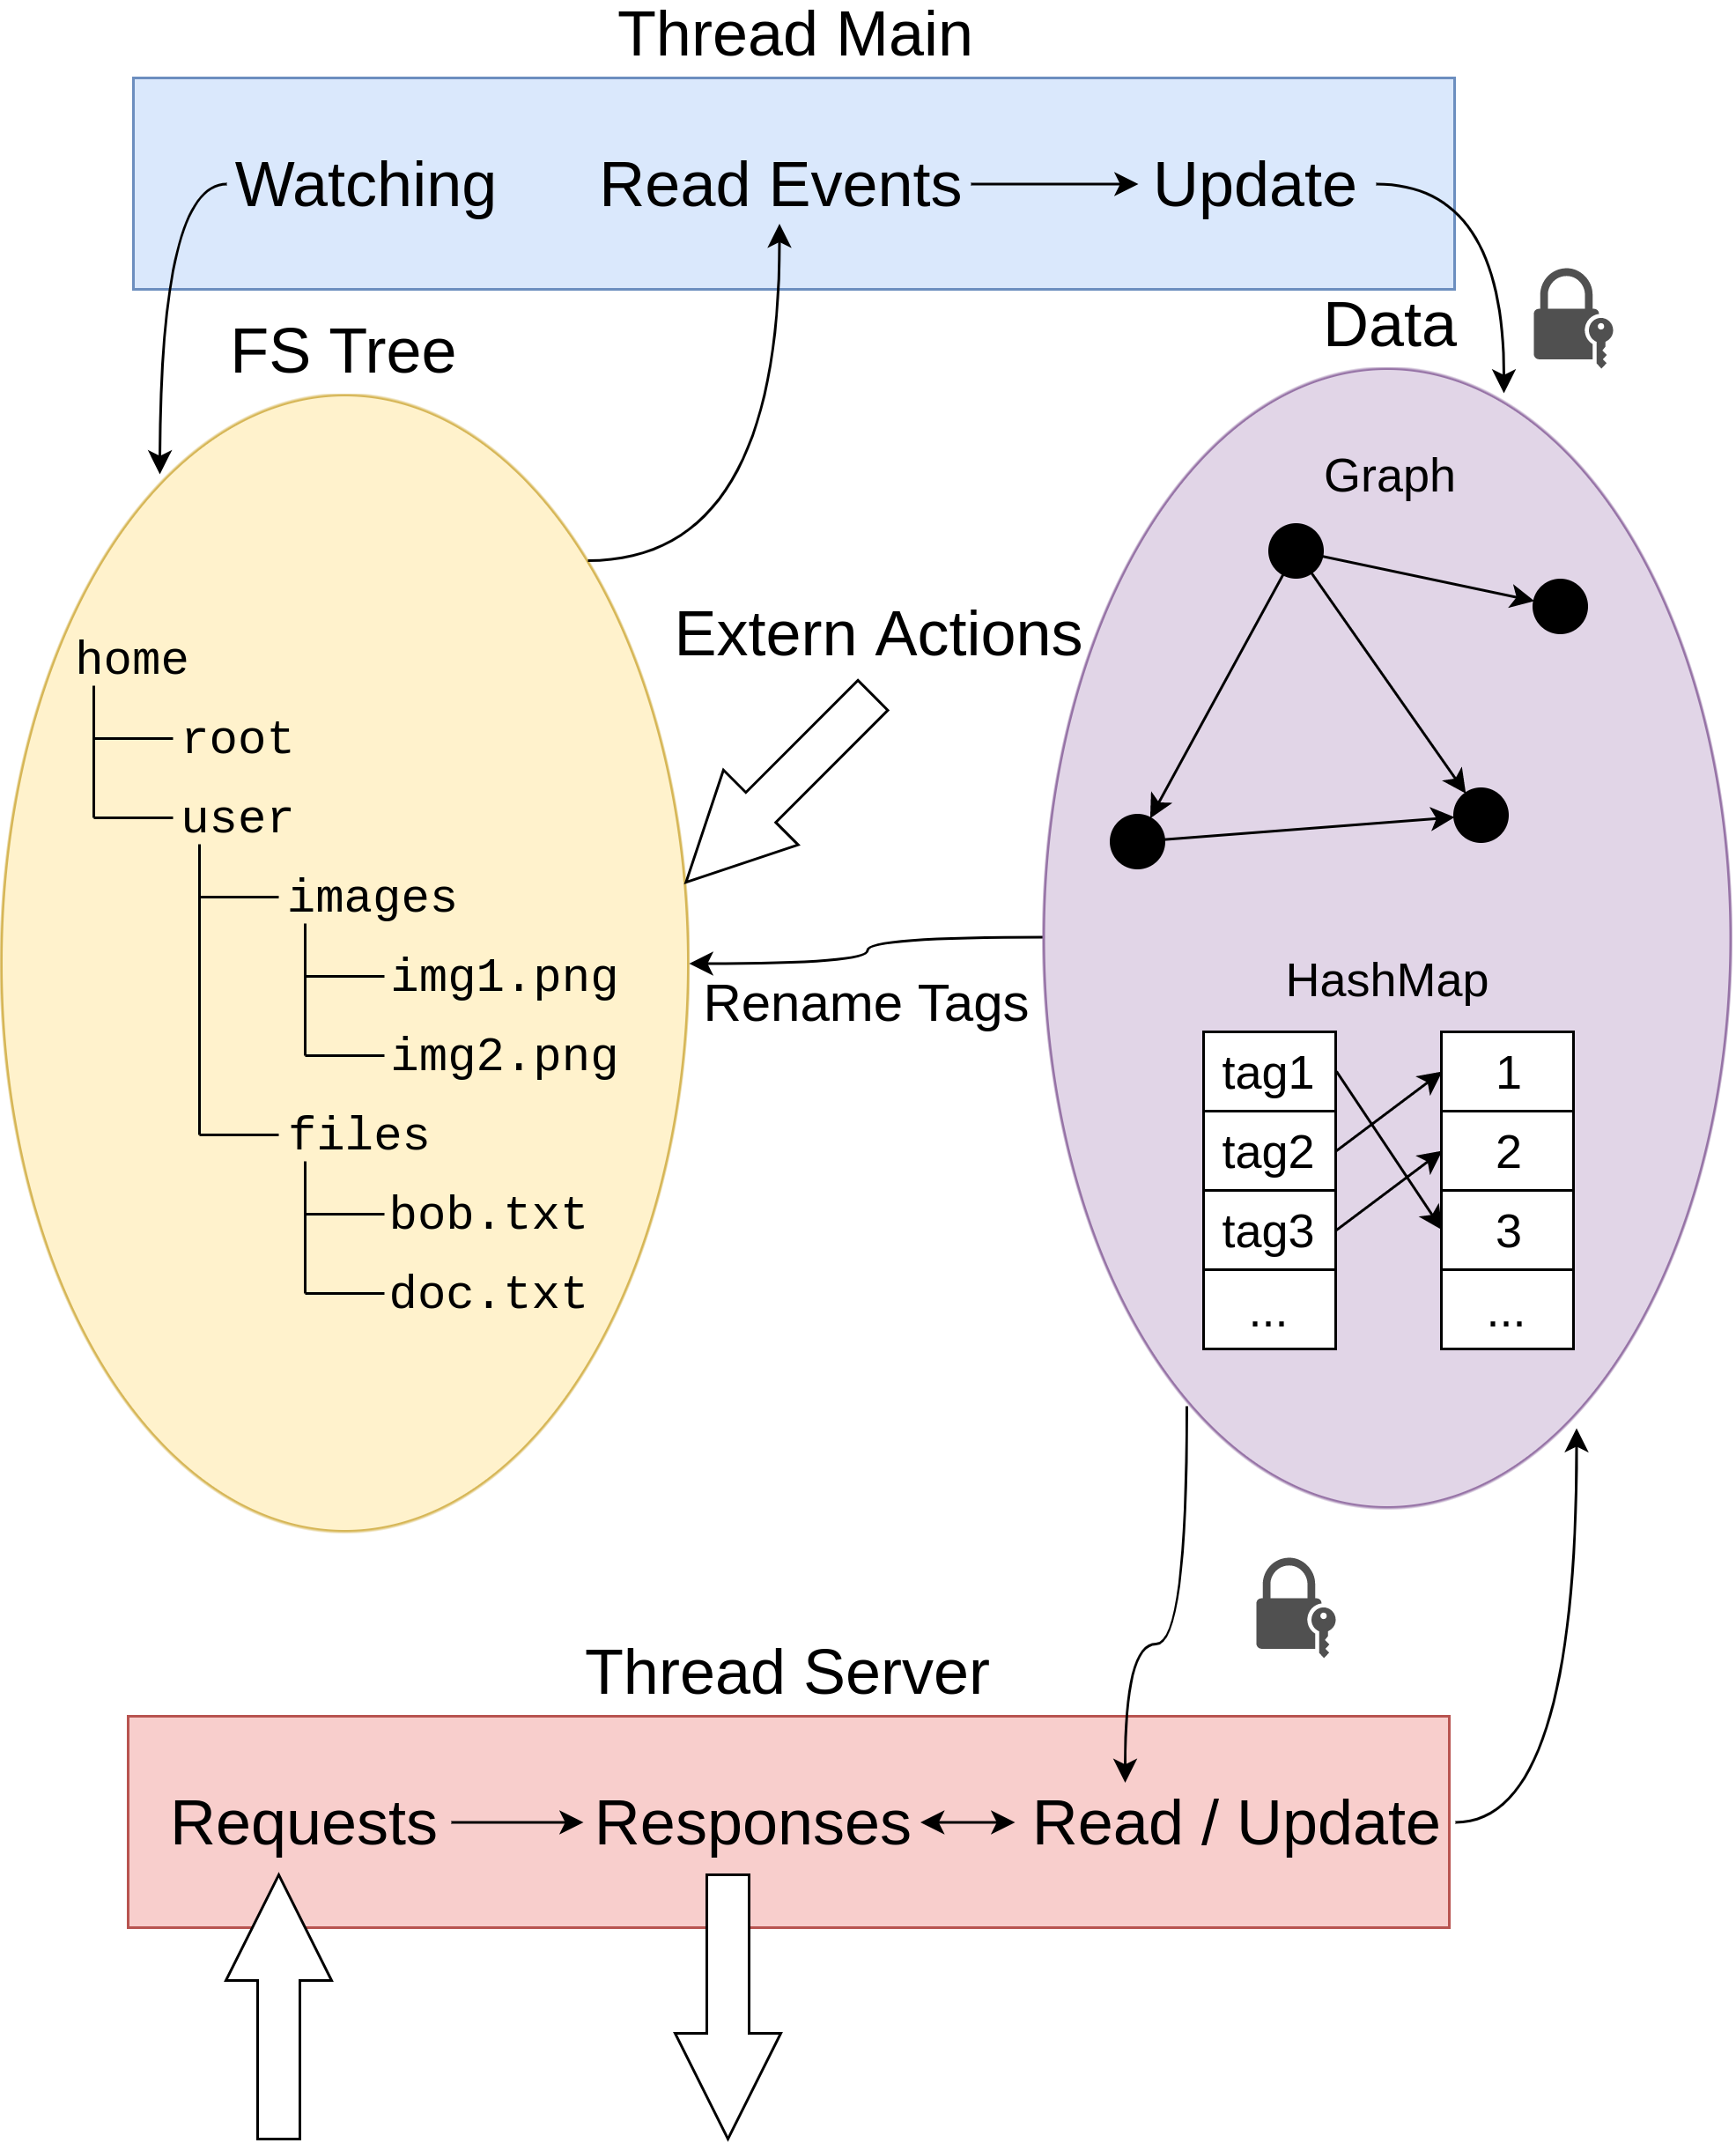
\includegraphics[width=1\textwidth]{images/tag_engine.png}
    \end{center}
    \caption{Schéma de fonctionnement de Tag Engine}
    \label{tag_engine_schema}
\end{figure}

%%%%%%%%%%%%%%%%%%%%%%%%%%%%%%%%%%%%%%%%%%%%%%%%%%%%%%%%%%%%%%%%%%%%%%%%%%%%%%%%%%%%%%%%%%%%%%%%%%%
%%%%%%%%%%%%%%%%%%%%%%%%%%%%%%%%%%%%%%%%%%%%%%%%%%%%%%%%%%%%%%%%%%%%%%%%%%%%%%%%%%%%%%%%%%%%%%%%%%%
\newpage
\subsubsection{Utilisation du programme et exemples}
Le programme attend un chemin absolu valide pointant vers un répertoire. Il admet un argument 
facultatif, \mintinline{text}{-d} ou \mintinline{text}{--debug}, qui imprime sur la sortie 
standard l'état du graphe et de la \textit{hashmap} et écrit deux fichiers, \mintinline{text}{graph.dot} 
et \mintinline{text}{graph.png}, après chaque événement survenu. Le listing \ref{tag_engine_ex} montre les 
\textit{outputs} de Tag Engine correspondants aux opérations sur l'arborescence manipulée par 
Tag Manager (voir section \ref{tag_manager_utilisation} et le listing \ref{tag_manager_ex}). 
On aperçoit aux lignes 11 à 16 l'ajout des tags "in\_a" et "myfiles" et aux lignes 30 et 31 les 
requêtes de tags et d'entrées effectuées.
Les deux fichiers représentent également l'état du graphe. Le fichier \mintinline{text}{graph.dot} 
respecte la syntaxe d'un outil appelé Graphviz \cite{ref50}, dédié à la modélisation et visualisation 
de graphes. Il comprend plusieurs moteurs de génération de graphes à partir de données texte ou 
brutes, dont \mintinline{bash}{dot} utilisé ici. À partir du fichier \mintinline{text}{graph.dot}, disponible au 
listing \ref{tag_engine_petgraph_dot}, la figure \ref{tag_engine_petgraph_dot_image} est obtenue. 
petgraph donne la possibilité de générer un fichier respectant la sémantique attendue par \mintinline{bash}{dot} 
pour dessiner un graphe. Nous pouvons voir que le résultat obtenu concorde avec l'arborescence obtenue.
\bigbreak
\begin{code}
    \inputminted[bgcolor=mygray,breaklines,breaksymbol=,linenos,frame=single,stepnumber=1,
        tabsize=2]{bash}{text/tag_engine_ex.txt}
    \caption{Exemple d'utilisation de Tag Engine}
    \label{tag_engine_ex}
\end{code}
\bigbreak
\bigbreak
\begin{code}
    \inputminted[bgcolor=mygray,breaklines,breaksymbol=,linenos,frame=single,stepnumber=1,
        tabsize=2]{text}{text/graph.dot}
    \caption{Fichier \mintinline{text}{dot} produit par petgraph}
    \label{tag_engine_petgraph_dot}
\end{code}
\bigbreak
\begin{figure}
    \begin{center}
        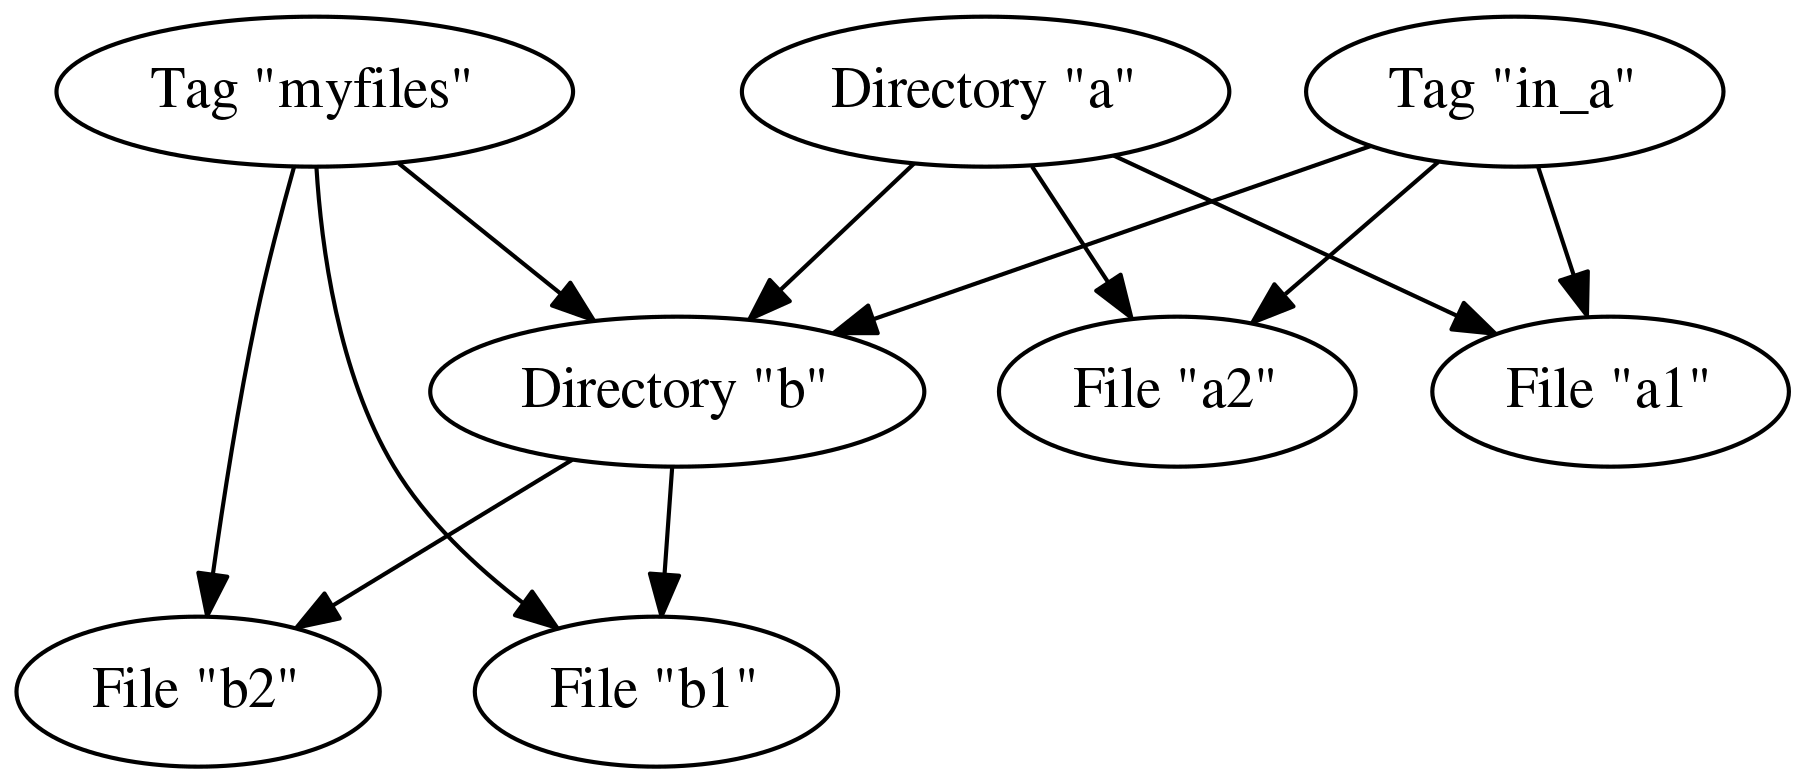
\includegraphics[width=1\textwidth]{images/graph.png}
    \end{center}
    \caption{Image du graphe obtenue avec la commande \mintinline{bash}{dot}}
    \label{tag_engine_petgraph_dot_image}
\end{figure}

%%%%%%%%%%%%%%%%%%%%%%%%%%%%%%%%%%%%%%%%%%%%%%%%%%%%%%%%%%%%%%%%%%%%%%%%%%%%%%%%%%%%%%%%%%%%%%%%%%%
%%%%%%%%%%%%%%%%%%%%%%%%%%%%%%%%%%%%%%%%%%%%%%%%%%%%%%%%%%%%%%%%%%%%%%%%%%%%%%%%%%%%%%%%%%%%%%%%%%%
\subsection{TagFS}
La figure \ref{tagfs_schema} résume le fonctionnement global du système TagFS, comportant Tag Manager et Tag Engine : 
\begin{enumerate}
    \item Gestion des tags avec Tag Manager.
    \item Indexation et surveillance de l'arborescence et serveur avec Tag Engine.
\end{enumerate}
\begin{figure}
    \begin{center}
        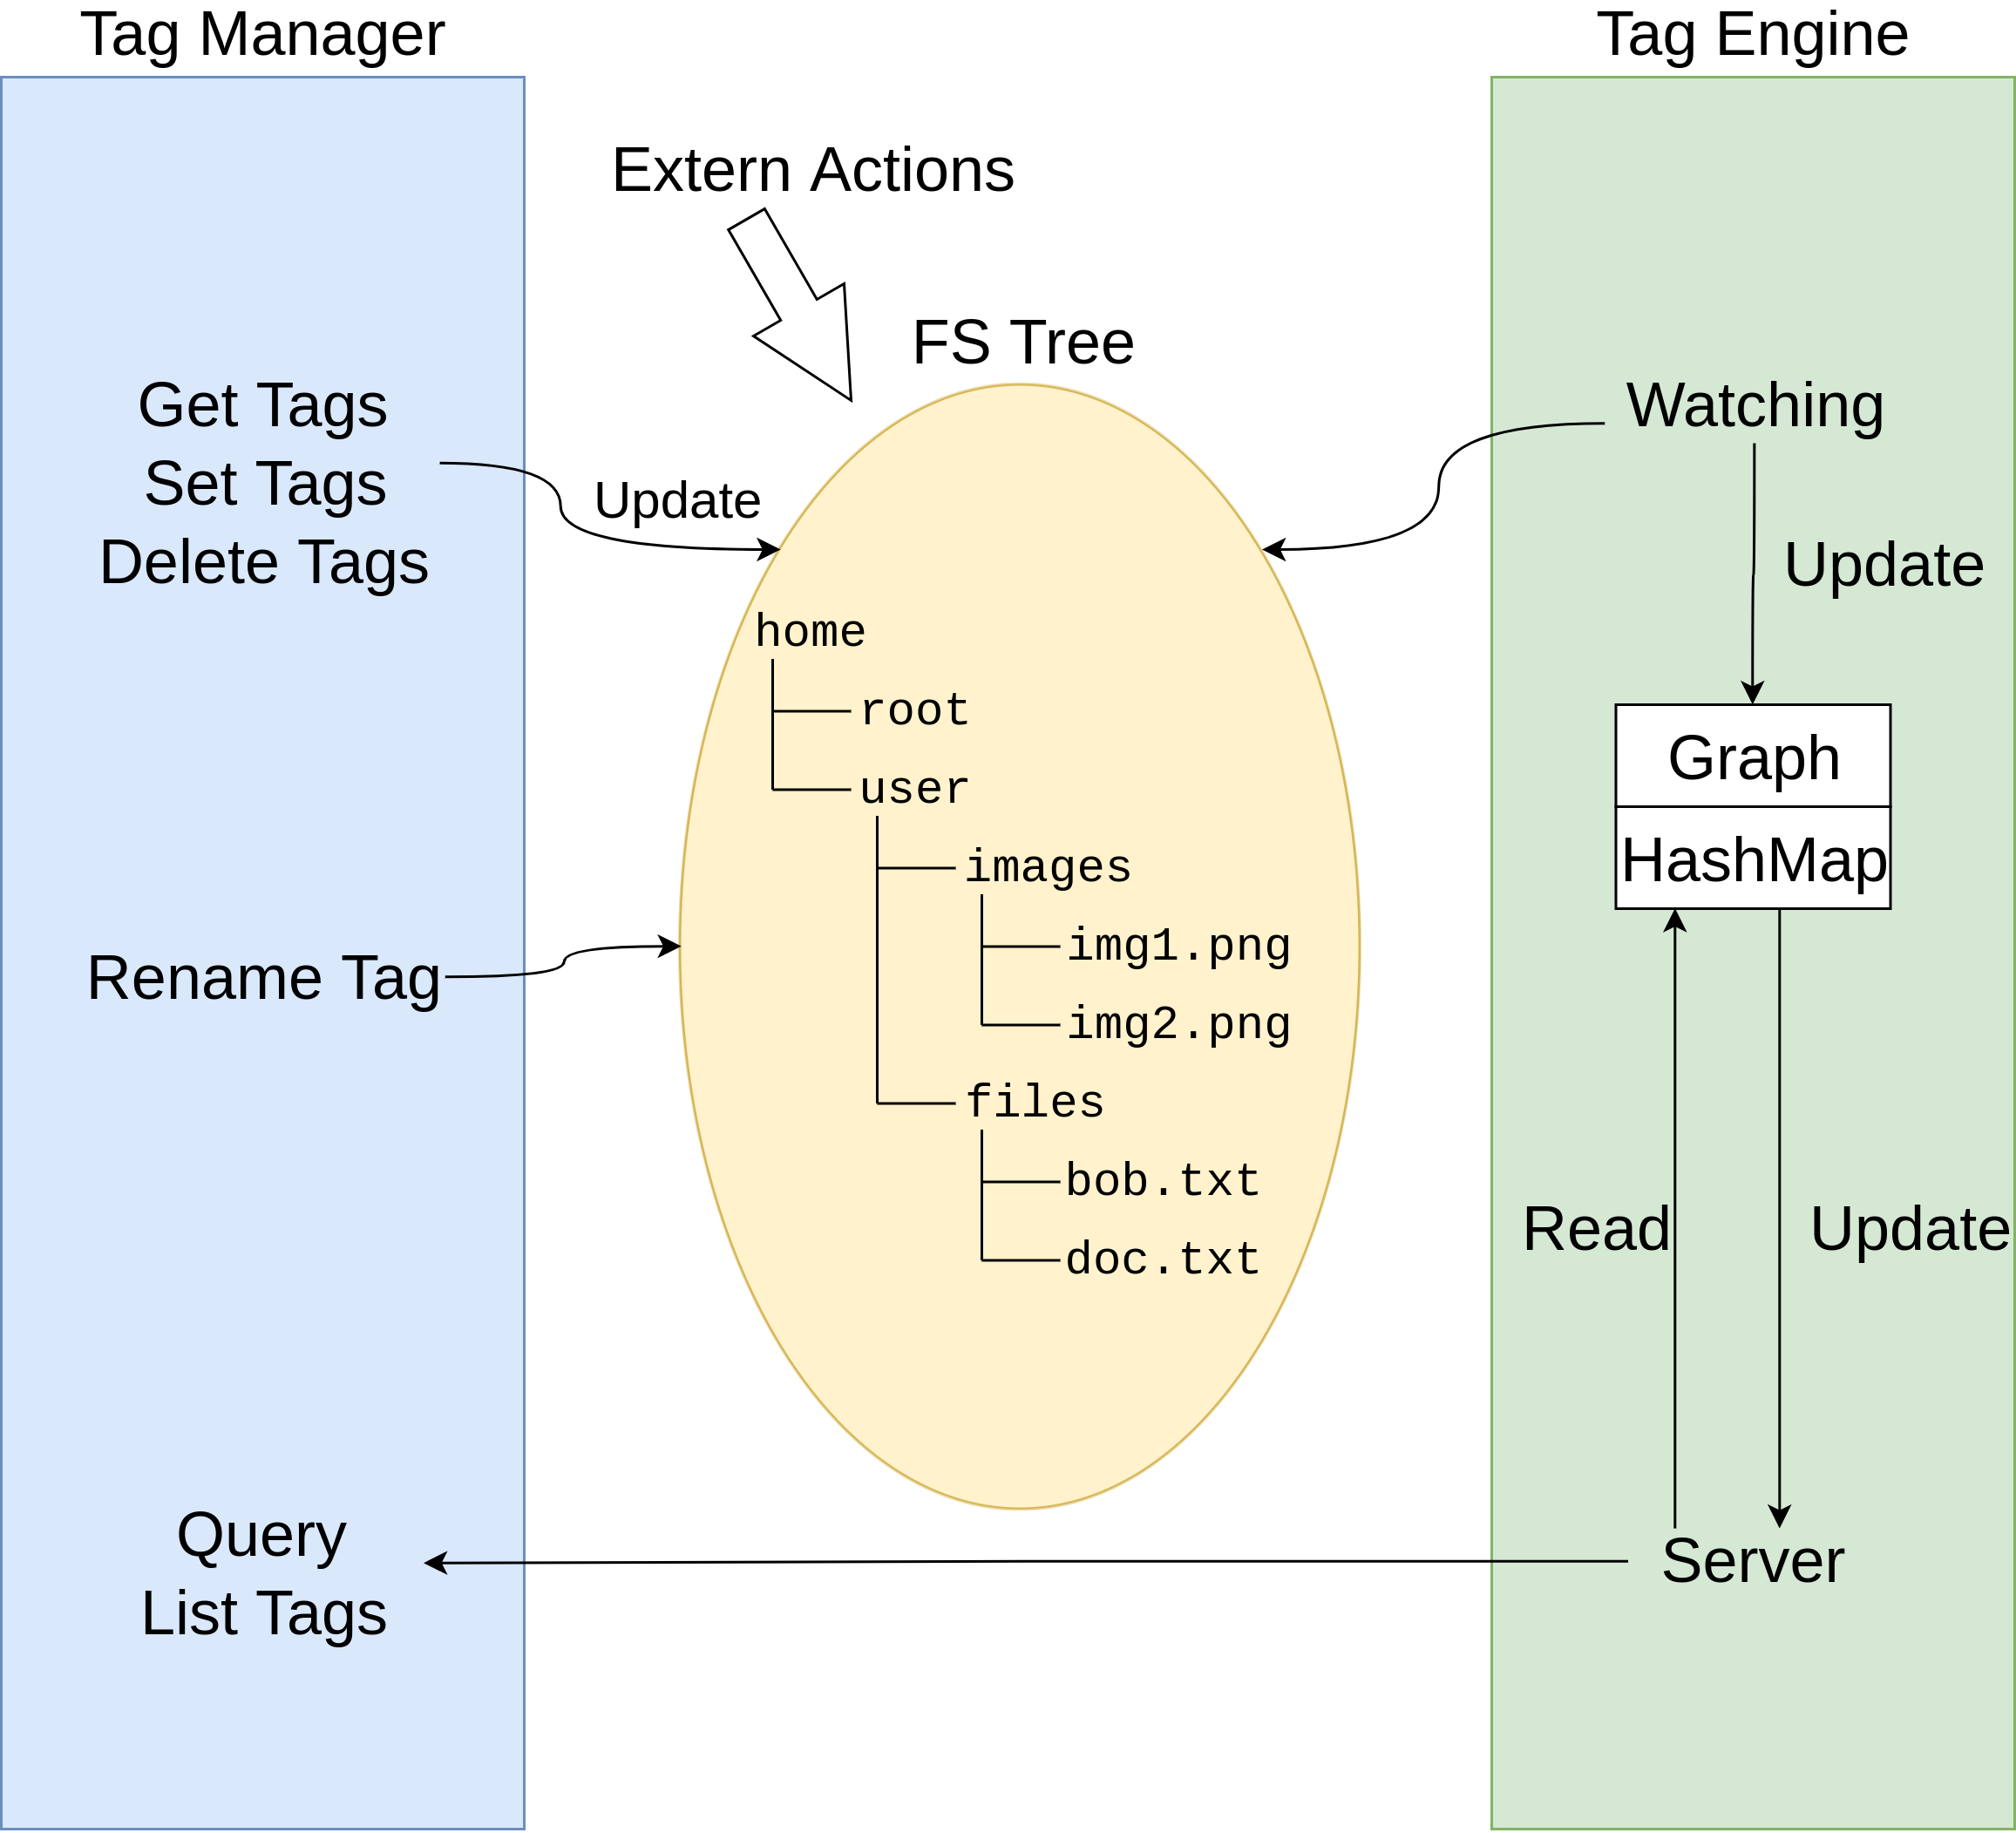
\includegraphics[width=1\textwidth]{images/tagfs.png}
    \end{center}
    \caption{Schéma de fonctionnement global de TagFS}
    \label{tagfs_schema}
\end{figure}

\newpage

\section{Tests} %-----------------------------------------------------------------------------------------------
%%%%%%%%%%%%%%%%%%%%%%%%%%%%%%%%%%%%%%%%%%%%%%%%%%%%%%%%%%%%%%%%%%%%%%%%%%%%%%%%%%%%%%%%%%%%%%%%%%%
%%%%%%%%%%%%%%%%%%%%%%%%%%%%%%%%%%%%%%%%%%%%%%%%%%%%%%%%%%%%%%%%%%%%%%%%%%%%%%%%%%%%%%%%%%%%%%%%%%%
\subsection{Mesures de performances}\label{mesures_performances}
Des mesures de temps d'exécution ont été réalisées avec une version de Tag Engine légèrement modifiée :
la fonction main a été tronquée à partir du lancement du thread socket serveur et de la boucle infinie 
écoutant sur les événements survenus sur l'arborescence surveillée. Ainsi, le programme parcoure 
une seule fois l'arborescence et construit le graphe et la table de hachage associée. Cette modification 
a été faite dans le but de mesurer plusieurs exécutions du programme pour un répertoire donné pour 
réaliser une moyenne du temps. Elle est illustrée au listing \ref{tests_main_modif}. 
\bigbreak
\begin{code}
    \begin{minted}[bgcolor=mygray,breaklines,breaksymbol=,linenos,frame=single,stepnumber=1,tabsize=2]{rust}
fn main() {
    // ...
    let now = Instant::now();
    let (graph, tags_index, root_index) = 
        tag_engine::graph::make_graph(
            String::from(absolute_path_root), base_path.clone()
        );
    let new_now = Instant::now();
    let elapsed = new_now.duration_since(now);
    println!("{}", elapsed.as_secs() as f64 + 
        elapsed.subsec_nanos() as f64 * 1e-9);
}
    \end{minted}
    \caption{\mintinline{rust}{main.rs} de Tag Engine modifié pour mesurer le temps d'exécution}
    \label{tests_main_modif}
\end{code}
\bigbreak
En tout, 200 exécutions ont été réalisées, 100 avec le programme compilé 
en mode \textit{debug} (\mintinline{bash}{cargo build}, non optimisé) et 100 avec le programme 
compilé en mode \textit{release} (\mintinline{bash}{cargo build --release}, avec optimisations maximum).
Les versions de Cargo et rustc sont les suivantes : cargo 0.26.0 (41480f5cc 2018-02-26) et rustc 1.25.0 (84203cac6 2018-03-25).
Les répertoires cibles diffèrent grandement dans leur nombre de sous-répertoires et fichiers contenus, allant 
de cinq répertoires et 863 fichiers à plusieurs milliers de répertoires et une centaine de milliers 
de fichiers (15'172 répertoires et 112'046 fichiers précisément). Ces répertoires ne contiennent 
pas de tags. Le tableau \ref{tests_directories} dresse les répertoires utilisés et leur contenu.
\begin{center}
    \begin{tabularx}{13cm}{|X|X|X|} \hline
        \textbf{Répertoire} & \textbf{Nombre de répertoires} & \textbf{Nombre de fichiers} \\ \hline
        Android & 15'172 & 112'046 \\ \hline
        android-studio & 3'331 & 13'287 \\ \hline
        bin & 553 & 9'306 \\ \hline
        Documents & 15'442 & 64'486 \\ \hline
        Dropbox & 2'377 & 8'659 \\ \hline
        Images & 5 & 863 \\ \hline
        Musique & 135 & 1'352 \\ \hline
    \end{tabularx}
    \captionof{table}{Répertoires utilisés pour les mesures de temps d'exécution}
    \label{tests_directories}
\end{center}
Le script \mintinline{bash}{bash} utilisé pour réaliser ces 200 exécutions est montré au listing 
\ref{script_bash_measures}. Il écrit pour chaque répertoire deux fichiers contenant les mesures des 100 exécutions 
pour les deux versions compilées du programme. La dernière boucle du script exécute le fichier 
\mintinline{octave}{average.m}, disponible au listing \ref{script_octave_moyenne}, qui fait la 
moyenne des 100 mesures.
La machine utilisée pour compiler et exécuter les mesures a les caractéristiques matérielles et 
logicielles suivantes (les commandes \mintinline{bash}{lscpu}, \mintinline{bash}{lshw}, 
\mintinline{bash}{uname -r} et \mintinline{bash}{lsb_release -a} ont été utilisées) :
\begin{itemize}
    \item Processeur : Intel(R) Core(TM) i7-3770K CPU @ 3.50GHz, boost @ 3.90GHz, x86\_64, 4 coeurs, 8 threads.
    \item Mémoire vive : 4x4 Go DDR3 1333 MHz.
    \item Carte mère : Asus Maximus V Formula, Chipset Intel(R) Z77.
    \item Disque système : Samsung 850 EVO Basic 500 Go.
    \item \acrshort{os} : Linux Mint 18.2 Sonya, kernel 4.15.0-24-generic.
\end{itemize}
\bigbreak
\begin{code}
    \inputminted[bgcolor=mygray,breaklines,breaksymbol=,linenos,frame=single,stepnumber=1,
        tabsize=2]{octave}{../average.m}
    \caption{Script Octave pour calculer la moyenne des exécutions}
    \label{script_octave_moyenne}
\end{code}
\begin{code}
    \inputminted[bgcolor=mygray,breaklines,breaksymbol=,linenos,frame=single,stepnumber=1,
        tabsize=2]{bash}{../measures.sh}
    \caption{Script bash pour exécuter 100 mesures de temps d'exécution}
    \label{script_bash_measures}
\end{code}
\bigbreak
Les moyennes obtenues sont représentées à la figure \ref{histo}. L'axe des y représente le temps 
moyen d'exécution du programme. L'axe des x représente les sept répertoires utilisés pour ce test. 
Pour chaque répertoire, il y a une mesure du programme compilé en mode \textit{debug} (barre bleue) 
et une mesure du programme compilé en mode \textit{release} (barre orange). On remarque que les 
deux répertoires contenant le plus de fichiers, à savoir \mintinline{text}{Android} et 
\mintinline{text}{Documents}, sont ceux dont le temps d'exécution est le plus long. Globalement, 
moins un répertoire contient d'entrées, moins le temps d'exécution sera long. À deux répertoires 
équivalents en termes d'entrées, les variations qui peuvent survenir sont très certainement dûes 
au spécificités des fichiers contenus, comme leur taille sur le disque par exemple.
\begin{figure}
    \begin{center}
        \fbox{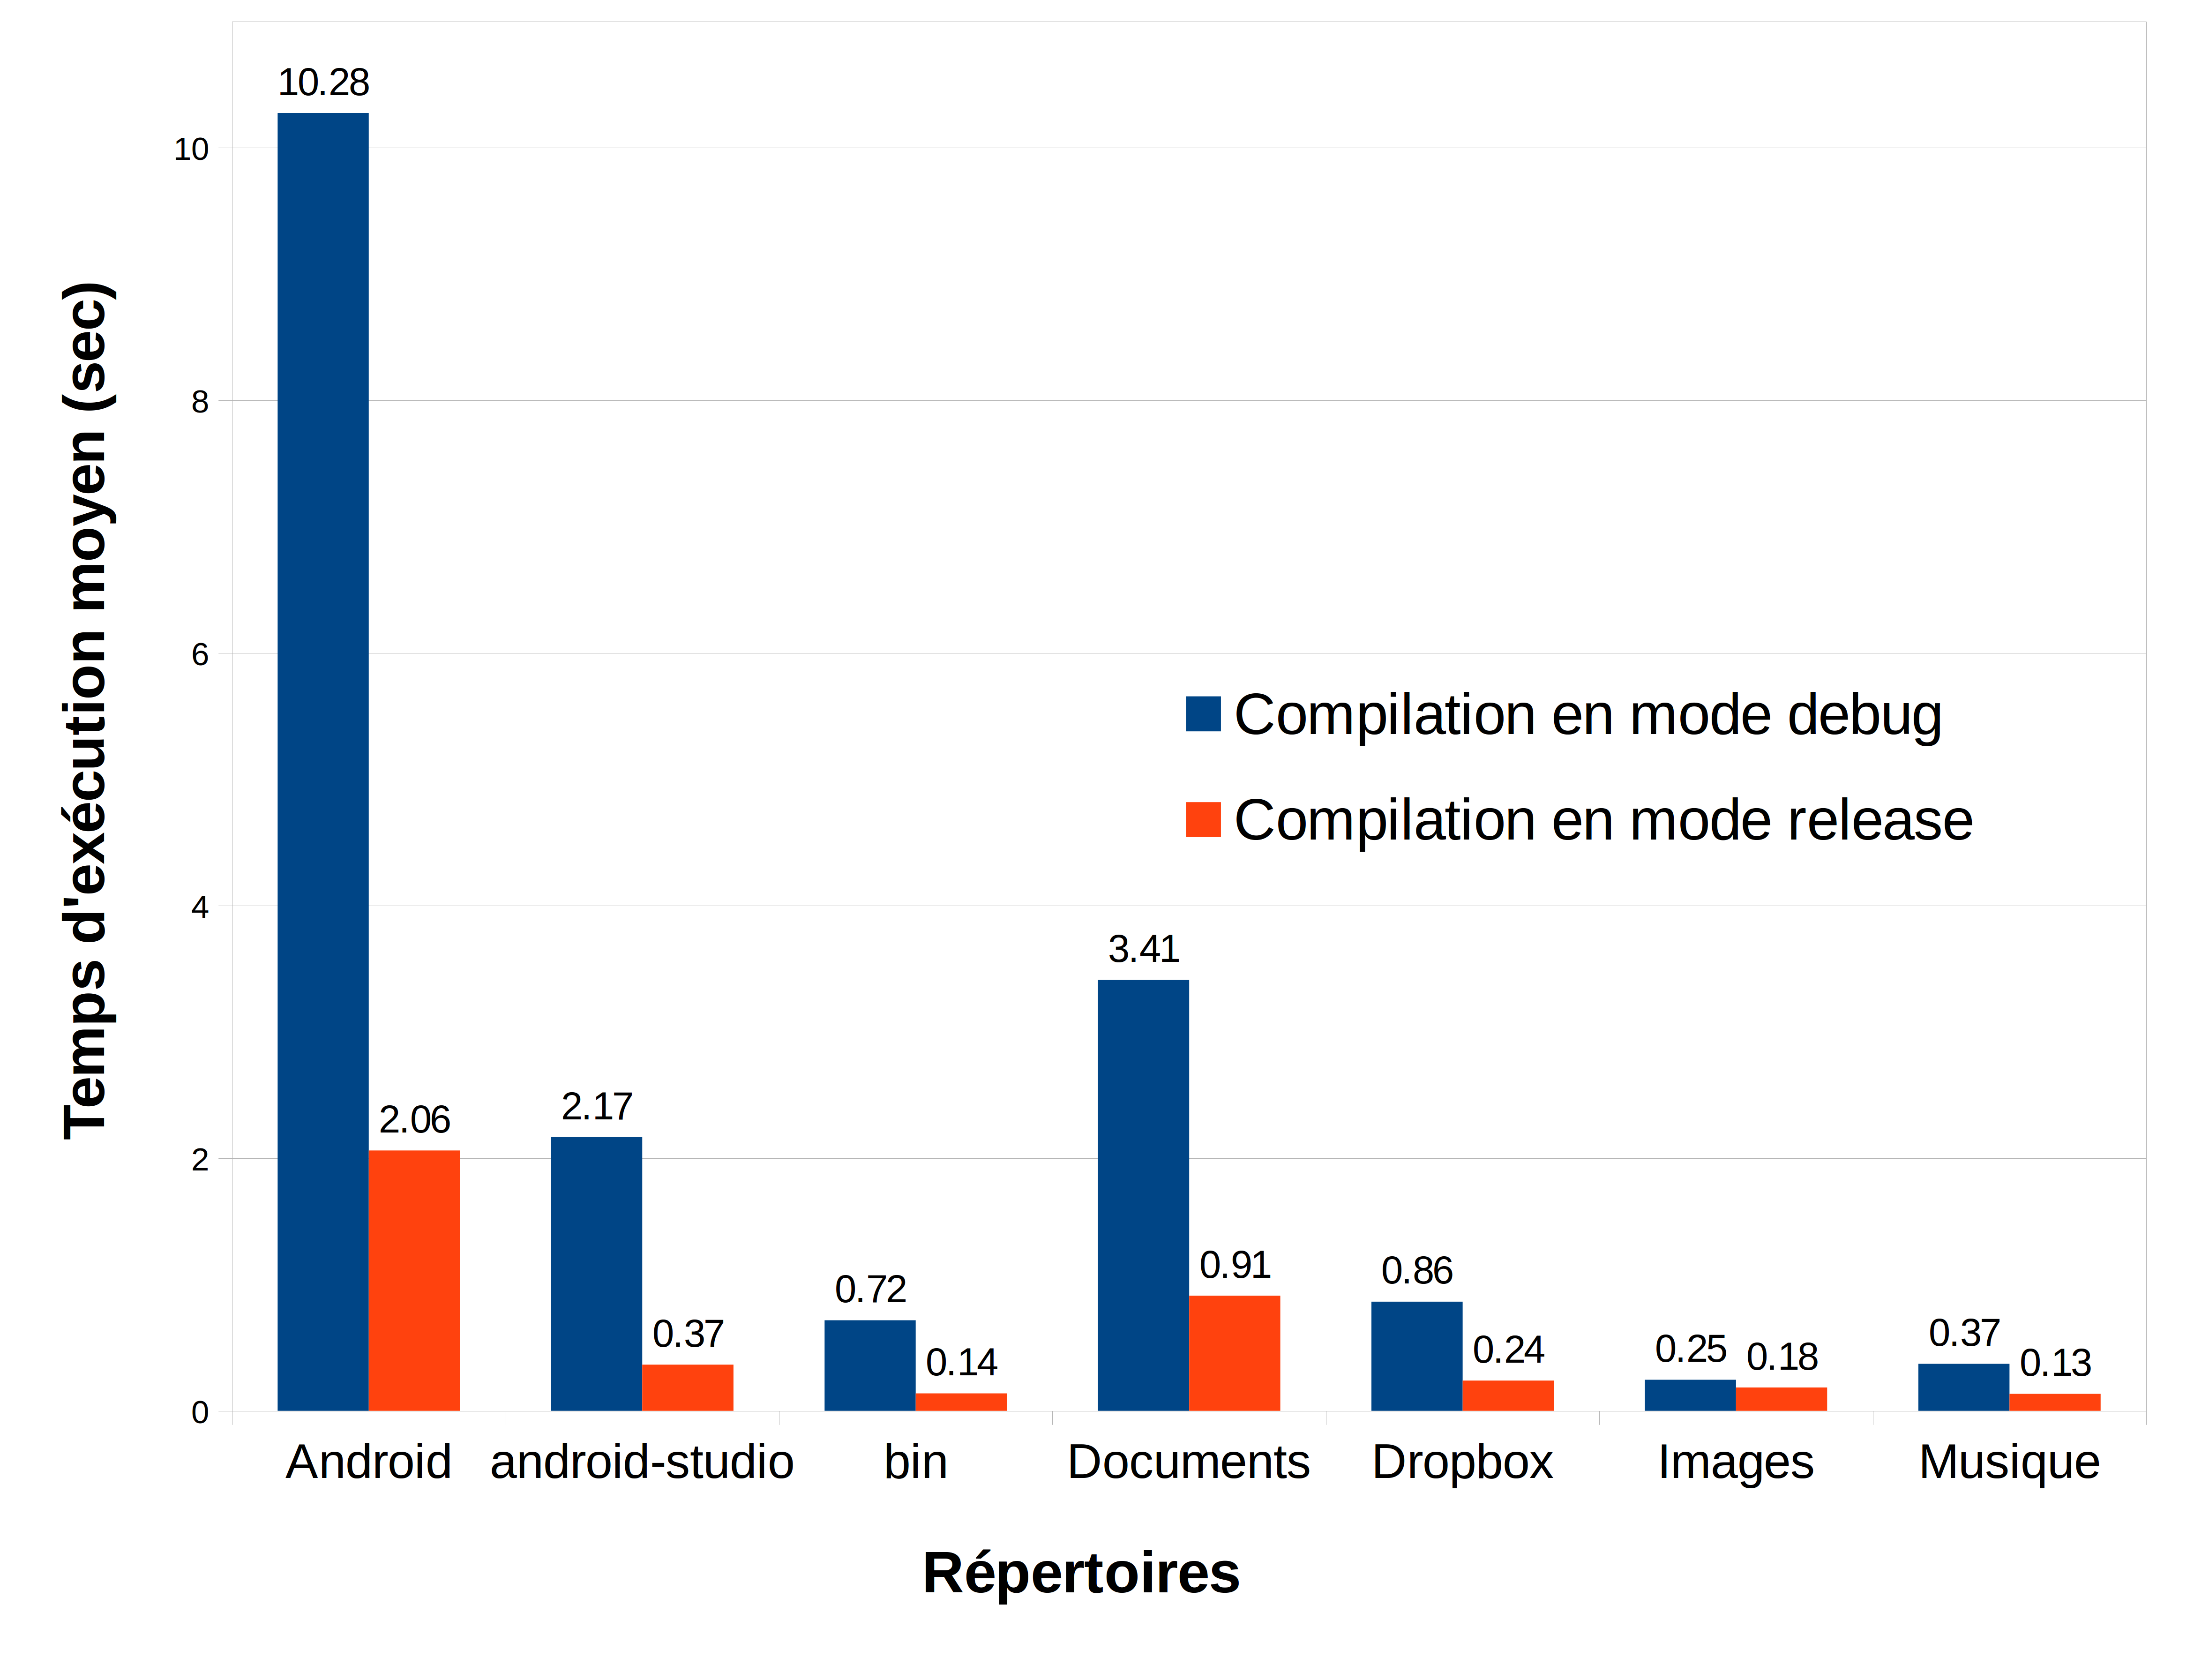
\includegraphics[width=1\textwidth]{images/histo.png}}
    \end{center}
    \caption{Temps d'exécution en fonction du répertoire}
    \label{histo}
\end{figure}
Il est intéressant de remarquer que le rapport de temps d'exécution entre la version non-optimisée 
et optimisée peut être important. La figure \ref{histo2} donne illustre ces rapports de temps. Nous 
voyons que la différence varie entre 5.93 pour \mintinline{text}{android-studio} et 1.33 pour 
\mintinline{text}{Images}, de manière générale ce sont à nouveau les répertoires 
avec le plus d'entrées qui ont les rapports les plus importants. Le répertoire \mintinline{text}{Images} 
contenant peu d'éléments en comparaison, il est difficile d'optimiser davantage le nombre 
également réduit d'opérations effectuées à l'exécution du programme. La leçon à tirer de ces rapports est 
que le compilateur Rust est capable de grandes optimisations sur le code.
\begin{figure}
    \begin{center}
        \fbox{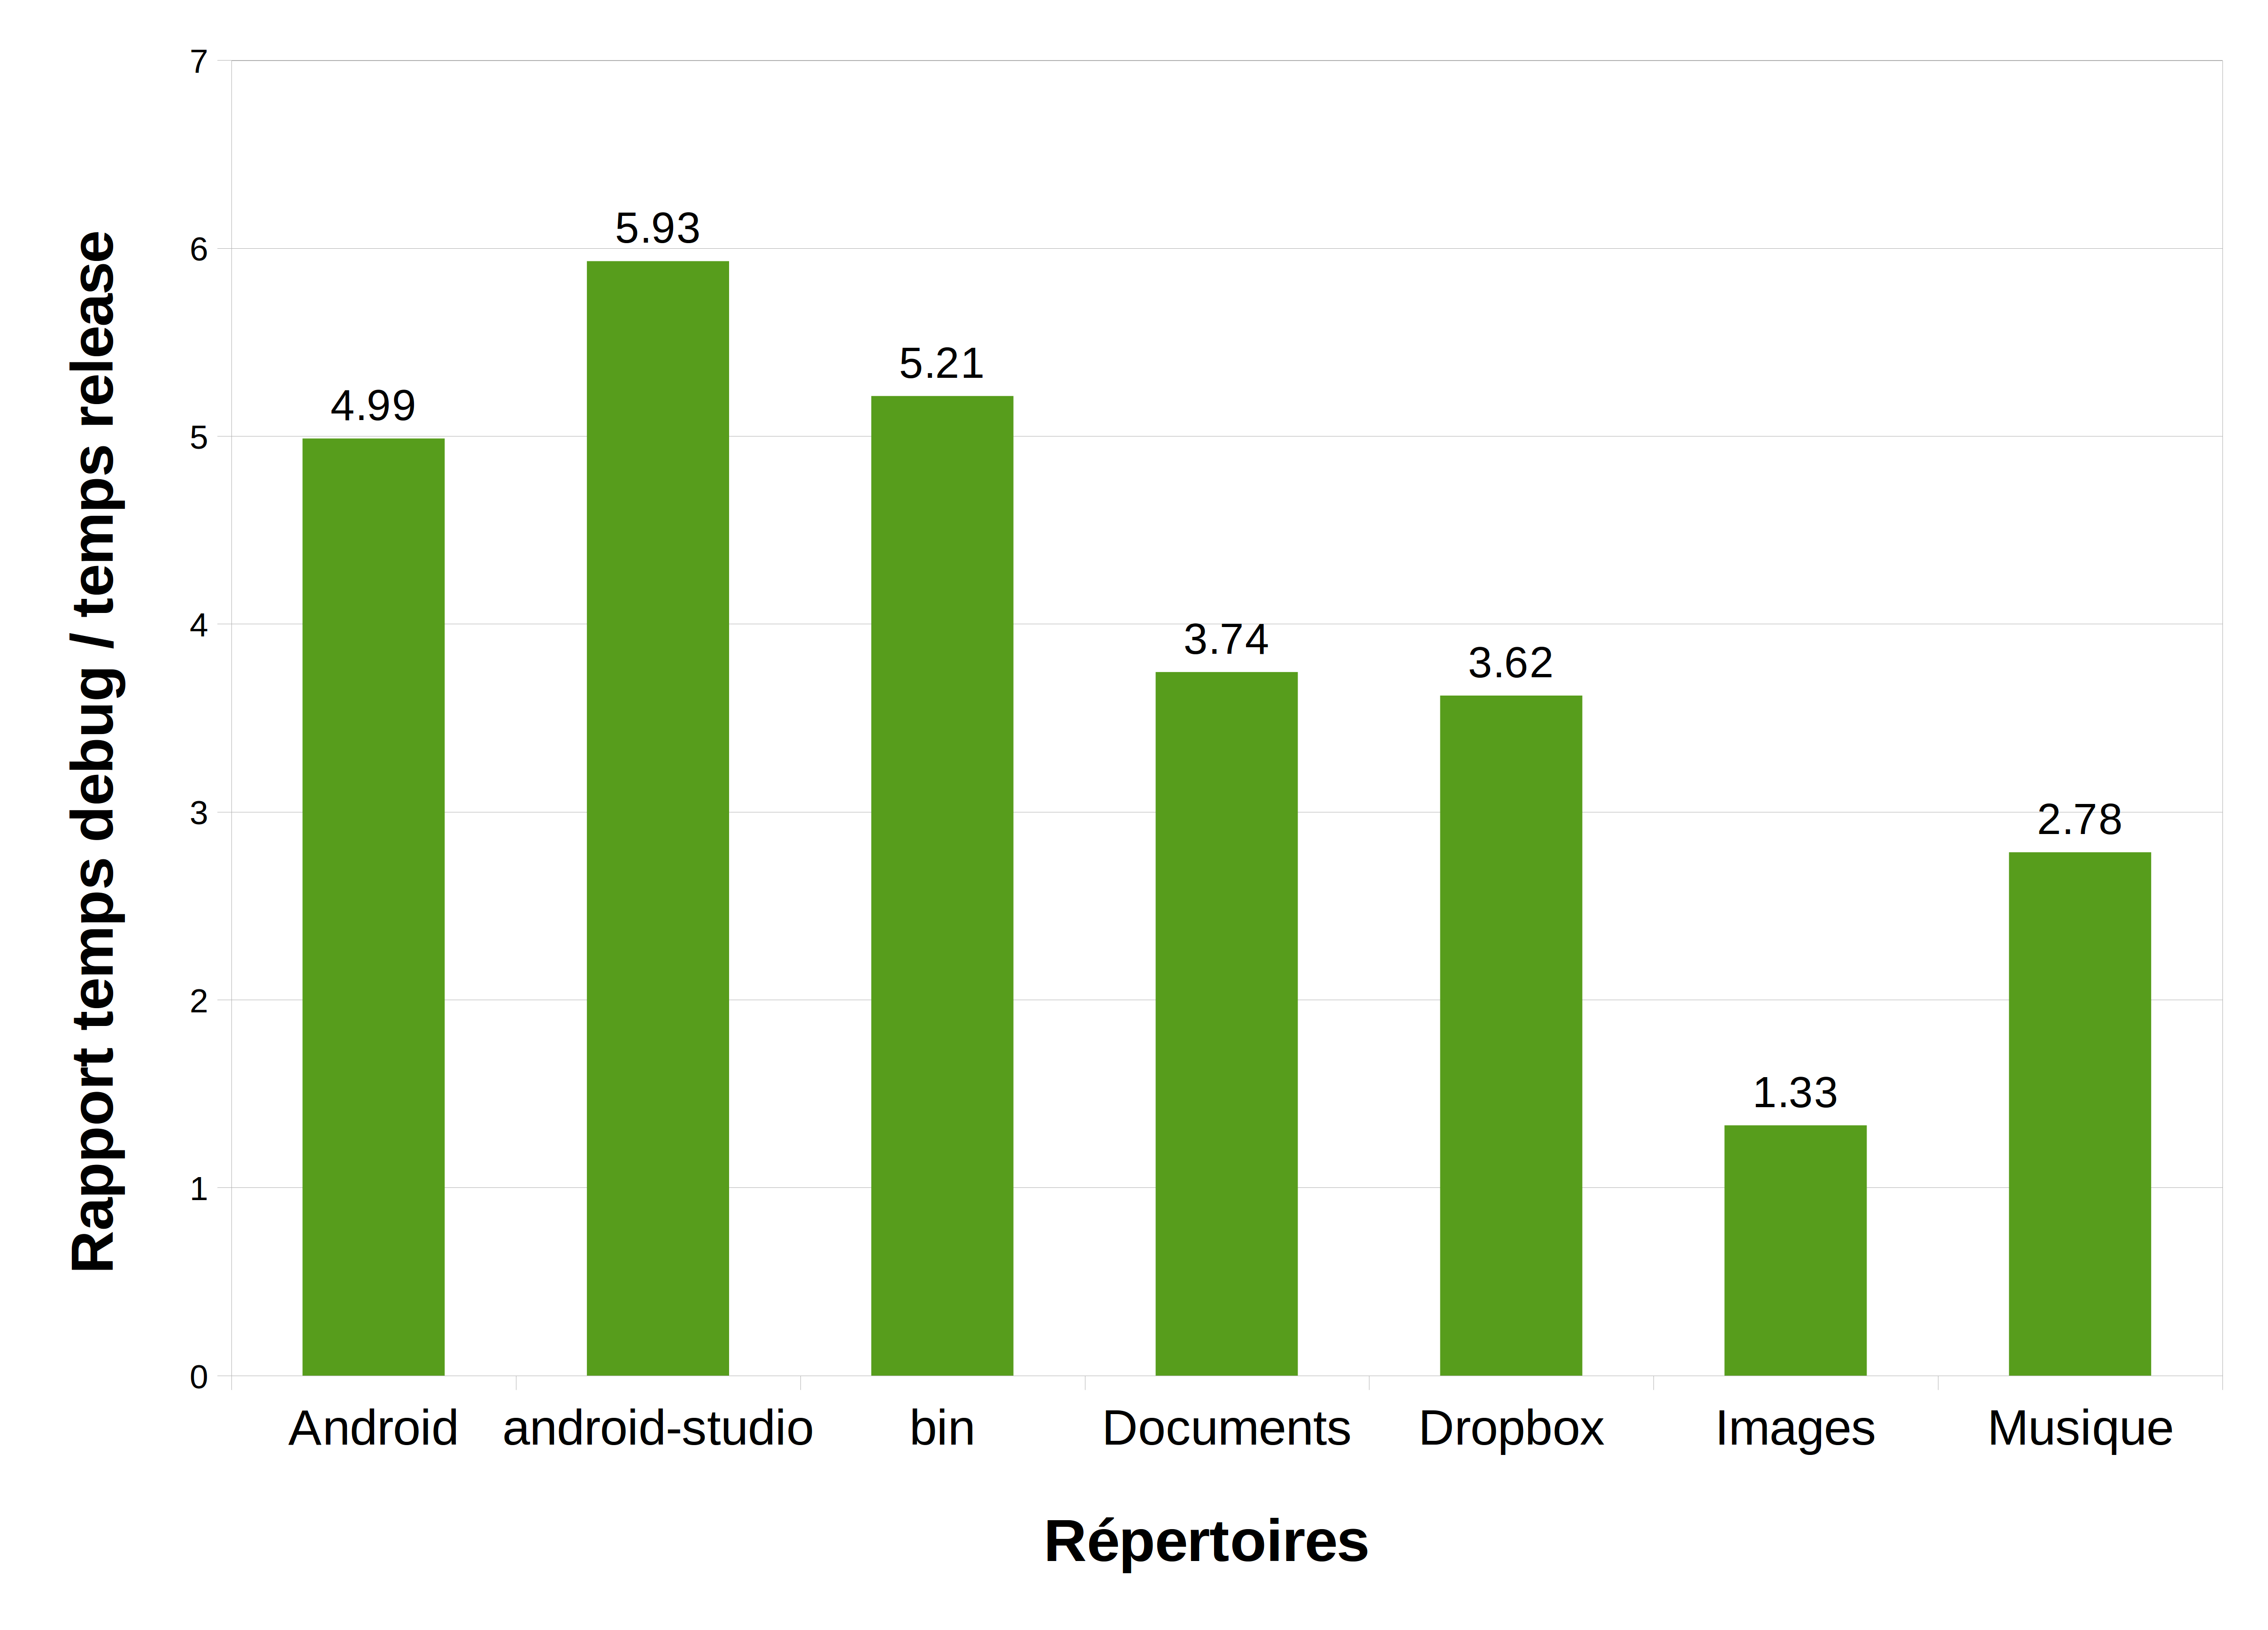
\includegraphics[width=1\textwidth]{images/histo2.png}}
    \end{center}
    \caption{Rapport entre le temps d'exécution en mode \textit{debug} et en mode \textit{release}}
    \label{histo2}
\end{figure}
%%%%%%%%%%%%%%%%%%%%%%%%%%%%%%%%%%%%%%%%%%%%%%%%%%%%%%%%%%%%%%%%%%%%%%%%%%%%%%%%%%%%%%%%%%%%%%%%%%%
%%%%%%%%%%%%%%%%%%%%%%%%%%%%%%%%%%%%%%%%%%%%%%%%%%%%%%%%%%%%%%%%%%%%%%%%%%%%%%%%%%%%%%%%%%%%%%%%%%%
\subsection{Tests unitaires avec Rust}
% TODO: tests unitaires supplémentaires

\newpage

\section{Discussion} %-----------------------------------------------------------------------------------------------
\begin{itemize}
    \item cahier des charges rempli ?
    \item réalisation OK ?
    \item performances
\end{itemize}
%%%%%%%%%%%%%%%%%%%%%%%%%%%%%%%%%%%%%%%%%%%%%%%%%%%%%%%%%%%%%%%%%%%%%%%%%%%%%%%%%%%%%%%%%%%%%%%%%%%
%%%%%%%%%%%%%%%%%%%%%%%%%%%%%%%%%%%%%%%%%%%%%%%%%%%%%%%%%%%%%%%%%%%%%%%%%%%%%%%%%%%%%%%%%%%%%%%%%%%
\subsection{Rust VS C}
%%%%%%%%%%%%%%%%%%%%%%%%%%%%%%%%%%%%%%%%%%%%%%%%%%%%%%%%%%%%%%%%%%%%%%%%%%%%%%%%%%%%%%%%%%%%%%%%%%%
%%%%%%%%%%%%%%%%%%%%%%%%%%%%%%%%%%%%%%%%%%%%%%%%%%%%%%%%%%%%%%%%%%%%%%%%%%%%%%%%%%%%%%%%%%%%%%%%%%%
\subsection{Bugs prob rencontrés}
\begin{itemize}
    \item Tentative d'implémentation arbre -> difficile -> switch vers graph 
    \item explications pourquoi c'est dur d'implémenter un arbre ou similaire \cite{ref2}
        \cite{ref26} \cite{ref46} \cite{ref47} \cite{ref48} \cite{ref49} \cite{ref50}
\end{itemize}
%%%%%%%%%%%%%%%%%%%%%%%%%%%%%%%%%%%%%%%%%%%%%%%%%%%%%%%%%%%%%%%%%%%%%%%%%%%%%%%%%%%%%%%%%%%%%%%%%%%
%%%%%%%%%%%%%%%%%%%%%%%%%%%%%%%%%%%%%%%%%%%%%%%%%%%%%%%%%%%%%%%%%%%%%%%%%%%%%%%%%%%%%%%%%%%%%%%%%%%
\subsection{Améliorations futures}
\begin{itemize}
    \item Environnement de bureau (Nautilus, Nemo) et/ou page web
    \item Daemon pour Tag Engine
    \item Ajouter des paths à surveiller après coup
    \item Clés USB
    \item Davantage de tests
\end{itemize}

\newpage

\section{Conclusion} %-----------------------------------------------------------------------------------------------
Les deux objectifs principaux de ce projet de Bachelor étaient d'étudier et s'approprier le 
langage Rust et de concevoir un moteur de gestion de tags efficace et \textit{user friendly}.
Rust est un langage moderne, fiable et performant. Ses atouts sont aussi nombreux que les nouveaux 
concepts qu'il introduit par rapport à un langage comme C. Fort d'une communauté active et sérieuse, 
il y a l'espoir qu'il soit adopté par de plus en plus de développeurs pour de nombreux types d'applications.
Bien que l'étude de Rust ait pris une grande partie du temps alloué à ce travail, ce ne fut pas du 
temps perdu. Les contraintes imposées par Rust devraient être un standard bénéfique pour de nombreux 
langages. 
\bigbreak
D'autres sujets ont été étudiés, comme les méthodes d'indexation, les attributs étendus des fichiers, 
ou les systèmes de surveillance du système de fichiers. Les limites des attributs étendus ont été 
montrées (notamment sur l'incompatiblité avec certains systèmes de fichiers ou partages réseaux) 
et du système de notification \mintinline{text}{inotify}, choisi pour ce projet. Néanmoins, ces 
deux technologies, avec l'association de Rust, ont permis de surpasser sur certains points les 
applications existantes de gestion des tags. Le cahier des charges demandé 
a été rempli et les interrogations sur l'usage de Rust dans ce genre d'applications vérifiées. 
Grâce à ce système, l'utilisateur peut maintenant étiqueter ses fichiers personnels sans avoir 
peur de les perdre et peut les retrouver facilement et rapidement selon des requêtes logiques 
simples. 
\bigbreak
Ce projet est le couronnement de mes études à hepia, il m'a fait découvrir un nouveau langage 
plein de potentiel, enseigné des bonnes pratiques de programmation et m'a fait progresser dans 
la démarche de conception et réalisation d'une application système. Tout le projet est disponible 
à cette adresse : \url{https://github.com/stevenliatti/tagfs}.

\newpage

\section{Références} %-----------------------------------------------------------------------------------------------
\bibliographystyle{unsrt}
\bibliography{bib}

\end{document}

% \begin{figure}
%     \begin{center}
%         \includegraphics[width=0.8\textwidth]{images/image.png}
%     \end{center}
%     \caption{légende}
%     \label{label}
% \end{figure}

% \bigbreak
% \begin{code}
%     \begin{minted}[bgcolor=mygray,breaklines,breaksymbol=,linenos,frame=single,stepnumber=1,tabsize=2]{rust}
% fn main() {
%     println!("Hello, world!");
% }
%     \end{minted}
%     \caption{Hello world en Rust}
%     \label{label}
% \end{code}
% \bigbreak

% \bigbreak
% \begin{code}
%     \inputminted[bgcolor=mygray,breaklines,breaksymbol=,linenos,frame=single,stepnumber=1,
%         tabsize=2,firstline=157,lastline=185]{rust}{file.rs}
%     \caption{légende}
%     \label{label}
% \end{code}
% \bigbreak
